\documentclass[
    %uninadraft,
    %colorlinks, 
    blacklinks,
    %palatino,
    libertine,
    %mathpazo,
    %tgschola,
    %tgscholamathpazo,
    %alegreya
]{uninathesis}

%\AtBeginDocument{\addtocontents{toc}{\protect\thispagestyle{empty}}} %remove page number from toc

\usepackage[english]{babel}
\addto\captionsenglish{% Replace "english" with the language you use
  \renewcommand{\contentsname}%
    {\sffamily Contents}%
}
\let\openbox\relax
\usepackage{amsthm}
\usepackage{proof}


% Math
\RequirePackage{mathtools}
\RequirePackage{mathrsfs} %need this for mathscr
\let\openbox\relax
\RequirePackage{amsthm}
\RequirePackage{stmaryrd} %for \llbracket

\theoremstyle{plain}
\newtheorem{theorem}{Theorem}

\theoremstyle{definition}
\newtheorem{definition}{Definition}
\newtheorem{example}{Example}

% Tikz - may be removed if unneeded
\RequirePackage{tikz}
\RequirePackage{pgfplots}
\pgfplotsset{compat=1.16}
\usetikzlibrary{positioning,automata,calc,fit,shapes,backgrounds,arrows.meta}
\usepackage{makecell}

% Miscellanea Packages
\RequirePackage[utf8]{inputenc}
\usepackage{ marvosym } %/Lightning
%\usepackage{ stmaryrd } %/lightning
%\usepackage[htt]{hyphenat}
\usepackage{subcaption} %subfigures

% read configuration file
%double quote command
\newcommand\dquote[1]{``#1''}
\newcommand\dquoteit[1]{``\emph{#1}''}

%single quote command
\newcommand\squote[1]{`#1'} %can write your macros here

% Bibliography
\RequirePackage{csquotes}
\RequirePackage[sorting=none,maxbibnames=4]{biblatex} %dashed=false to remove dashes on repeated authors.
\bibliography{_bib/bibliography.bib} %bib database(s)

% Front page (package uninafrontespizio)
\Universita{Università degli Studi di Napoli Federico II}
\Facolta{Scuola Politecnica e delle Scienze di Base}
\Dipartimento{Dipartimento di Ingegneria Elettrica e Tecnologie dell'Informazione}
\CorsoDiLaurea{Corso di Laurea Triennale in Informatica}
%\Materia{Verifica di Sistemi}
\AnnoAccademico{2024--2025}
\Titolo{Implementation of a decision procedure for the fluted fragment in Vampire}
\Relatore{Prof.\ Fabio \textsc{Mogavero}}
\Relatore{Prof.\ Massimo \textsc{Benerecetti}}
% \Relatore{Baronessa Filiguelli \textsc{de Bonchamps}}
\RelatoreLabel{Relatori}
\CorrelatoreLabel{}
\Candidato{Riccardo \textsc{Elena}}
\Matricola{N86/4490}
\Logo{logo-federico-II.pdf}
\LogoWidth{3.5cm}
\LogoPosition{below-uni}

%custom hyphenation
\hyphenation{ERTMS/ETCS}

% Theorem-like environments

\newtheorem{lemma}{Lemma}     % Shares numbering with theorems
\newtheorem{proposition}{Proposition}

% Optional: definitions and remarks with different style

\theoremstyle{remark}
\newtheorem{remark}[theorem]{Remark}

% Thesis specific custom commands

\newcommand{\landor}{\mathrel{\land\mkern-3mu\lor}}
\newcommand{\ms}{\,}
\NewDocumentCommand{\var}{m}{\text{var} (#1)}
\NewDocumentCommand{\flseq}{o m o}{(\overline{\IfValueTF{#1}{#1}{u}}_{#2}\IfValueTF{#3}{,#3}{})}
\NewDocumentCommand{\fldef}{m o m}{\text{Def}_{#1}\IfValueTF{#2}{^{#2}}{}(#3)} %chktex 36

\tikzset{
    syntree/.style={
        level distance=1.5cm,
        sibling distance=2.5cm,
        grow=down,
        % Stile per quantificatori (rettangolare)
        quantifier/.style={draw, rectangle, align=center, 
                           minimum width=1cm, minimum height=0.5cm, 
                           inner sep=2pt},
        % Stile per connettivi (diamond/rombo)
        connective/.style={draw, diamond, align=center, 
                          minimum width=1cm, minimum height=0.4cm,
                          inner sep=1pt},
        % Stile per literal/predicati (ellisse)
        literal/.style={draw, ellipse, align=center, 
                       minimum width=1cm, minimum height=0.4cm,
                       inner sep=1pt}
    }
}

\usepackage[title,titletoc]{appendix}

\begin{document}

    \pagestyle{empty}
    \frontmatter
    \makefrontespizio~\clearpage
    \makefrontespizioalt~\clearpage

    \pagestyle{backmatter}
    \chapter*{Abstract}

% This is the abstract.\blindtext[2]

% \chapter*{Sommario}
% Qui puoi inserire il sommario (la traduzione dell'abstract in italiano).
% \blindtext[2]
    
    \clearpage
    \tableofcontents

    \mainmatter{}

    \newpage\pagestyle{introduction}

% The \unnumberedchapter, \unnumberedsection commands provided by the uninathesis 
% documentclass add an unnumbered entry to the TOC.
% If you use the starred version of classic sectioning commands (e.g. \chapter*)
% no TOC entry will be added!

\chapter*{Introduction}
% \unnumberedsection{A first unnumbered section}

First-Order Logic (FOL) emerged from the mathematical foundations laid in \textit{Begriffsschrift}~\cite{frege1879} by \citeauthor{frege1879} and in \textit{Principia Mathematica}~\cite{russell1910} by \citeauthor{russell1910}, and has since become a cornerstone formalism in computer science.
Its formal yet expressive nature makes it particularly well-suited for computational reasoning across diverse domains.
In knowledge representation, FOL underpins semantic web technologies and ontology languages like OWL, enabling machines to reason about complex relationships in data.
Meanwhile, in verification, it serves as the logical foundation for model checkers and theorem provers that ensure software correctness, while in artificial intelligence, it historically powered automated reasoning systems and planning algorithms, though modern AI has largely shifted toward statistical and neural approaches that often lack the transparency and formal guarantees that FOL-based systems provide.

However, the expressive power of FOL comes at a cost: undecidability.
This was established independently in the 1930s by \citeauthor{church1936}~\cite{church1936} using the lambda calculus, and by \citeauthor{turing1936}~\cite{turing1936} via Turing machines---two distinct formalisms that captured the limits of computation.
Their results demonstrated that no algorithm can, in general, determine whether an arbitrary FOL formula is valid. This fundamental limitation creates a significant computational barrier for automated reasoning.
In response, two complementary research directions have emerged: the systematic identification of decidable fragments that retain sufficient expressiveness for practical applications, and the development of automated theorem provers (ATPs) that---while unable to guarantee termination on all inputs---employ sophisticated heuristics and optimizations to solve many real-world problems efficiently.

Among the most prominent ATPs for first-order logic is \textit{Vampire}~\cite{kovacs2013vampire}, a high-performance prover built on advanced saturation-based reasoning.
Vampire combines ordered resolution with literal selection, term indexing, and clause simplification techniques to explore the space of logical consequences efficiently.
It also incorporates modern enhancements such as efficient preprocessing, strategy scheduling, and support for first-order logic with built-in theories.
These features have made Vampire highly successful in competitive settings like the CADE ATP System Competition (CASC)\footnote{The CADE ATP System Competition (CASC) is the annual evaluation of fully automatic, classical logic, ATP systems --- the world championship for such systems.}, and effective in practical applications ranging from formal verification to software analysis.
Moreover, Vampire's extensible architecture and open-source nature make it the go-to choice for research and experimentation in the field of automated reasoning.

While general-purpose provers like \textit{Vampire} are designed to handle unrestricted first-order logic, certain decidable fragments offer opportunities for more targeted and efficient reasoning.
One such fragment is the \emph{Fluted Fragment}, distinguished by its strict syntactic discipline: variables in atomic formulas must follow the order in which they are quantified~\cite{quine1968predicate}.
This constraint, first introduced by Quine, limits expressiveness in some dimensions but crucially preserves decidability. Subsequent studies have shown that the Fluted Fragment occupies an interesting middle ground—more complex than many guarded or bounded-variable fragments, yet still admitting well-characterized decision procedures~\cite{pratt2019fluted}.
Applications have emerged in areas such as knowledge representation, database logic and computational linguistics, where the fragment’s regular structure aligns naturally with hierarchical or sequential data.
\uninatodo{I remember we discussed this application, but I cannot find the reference now.}
These properties make it a compelling candidate for specialized reasoning techniques that can outperform general ATPs in relevant domains.

A specialized reasoning technique for the Fluted Fragment is presented by \citeauthor{schmidt2000resolution} in their resolution-based decision procedure~\cite{schmidt2000resolution}.
Their approach characterizes fluted logic through a novel class of \emph{fluted clauses}, and introduces a calculus ---\textsc{R\textsuperscript{sep}}--- which extends ordered resolution with a dynamic renaming rule called \emph{separation}.
This rule enables the transformation of non-strongly fluted clauses into strongly fluted ones, thereby preserving a bounded number of variables and ensuring closure under resolution.
Crucially, the authors prove that their calculus is sound, complete, and terminating for fluted logic, establishing a resolution-based decision procedure for the fragment.

%This result not only deepens the understanding of the structural properties that make fluted logic decidable, but also provides a foundation for building dedicated automated reasoning tools that leverage the syntactic discipline of the fragment.

In this thesis, we implement this resolution-based decision procedure for the Fluted Fragment, with the goal of evaluating its practical effectiveness.
By faithfully realizing the \textsc{R\textsuperscript{sep}} calculus, including the separation rule and associated structural constraints, the implementation provides a concrete instantiation of the theoretical framework.
To assess the impact of fragment-specific optimization, we conduct an empirical comparison against the general-purpose theorem prover \textit{Vampire}, highlighting the potential advantages of tailored reasoning techniques for decidable fragments of first-order logic.

\unnumberedsection{About this thesis work}

This thesis retraces all the steps of the implementation of the resolution-based decision procedure for the Fluted Fragment mentioned above, starting from the theoretical foundations and culminating in the empirical evaluation of the implemented system.

The work is structured as follows:

\begin{description}
    \item[Chapter 1] provides an overview of the theoretical foundations of first-order logic, briefly discussing its structure and key concepts such as Skolemization, Naming, and Clausification.
    \item[Chapter 2] illustrates the main inference rules of a resolution-based decision procedure, highlighting the differences between their standard and their ordered versions. In particular, it covers the concept of \textit{liftable orders} and how they can be used for the definition of \textit{ordered inference rules}.
    \item[Chapter 3] describes the Fluted Fragment and the resolution-based decision procedure for it, detailing the separation rule and the structural constraints that ensure decidability. The chapter discusses the structure of the fluted formulae, the definition of fluted clauses, and the naming procedure that ensures the flutedness of the clauses.
    \item[Chapter 4] briefly analyses \textit{Vampire} and its architecture, focusing on relevant components for the implementation of the decision procedure. In detail, it discusses the \textit{Preprocessor}, the \textit{Saturation Algorithm}, and the \textit{Clause Selection} components.
    \item[Chapter 5] presents the implementation of the decision procedure, discussing the design choices made, and the challenges encountered during development, divided into three main parts covering the three main components of the implementation: the \textit{Classifier}, the \textit{Preprocessor}, and the \textit{Fluted Resolution}.
    \item[Chapter 6] discusses the results of the first evaluation, based on the TPTP library, highlighting the strengths and weaknesses of the implemented decision procedure. These problems have been selected using the \textit{Classifier} component and the evaluation is based on the comparison with the results of \textit{Vampire} and of a \textit{Hybrid model}, composed by the \textit{Fluted Preprocessor} and the \textit{Vampire Resolution}, on the same problems.
    \item[Chapter 7] discusses the results of the second evaluation, based on the automatically generated problems, as well as the design and implementation process of the problems generator and the evaluation framework. This evaluation required the implementation of another component, the \textit{Fluted Generator}, which is responsible for generating the problems to be solved by the decision procedure and by the other \textit{two models}.
    \item[Chapter 8] concludes the thesis, summarizing the main findings and discussing potential future work.
\end{description}





    \newpage\pagestyle{main}

    \chapter{First Order Logic}\label{chap:first-order-logic}

\inlineminitoc{}

\noindent First-order logic (FOL), or predicate logic, is a formal system used in mathematics, philosophy, linguistics, and computer science to express statements about objects and their relationships.
It uses \textbf{terms} for the representation of objects in the domain of discourse and \textbf{predicates} to express properties of these objects or relationships between them.
Moreover, FOL allows for the use of \textbf{quantifiers} to make statements that apply to all objects (universal quantification) or some objects (existential quantification) in the domain, and \textbf{logical connectives} to construct more complex statements.

One well-known informal statement, \dquote{All humans are mortal} for example, can be expressed in FOL as:
\begin{equation*}
    \forall x \left( \text{H}(x) \implies \text{M}(x) \right)
\end{equation*}

Syntactically speaking, this sentence is composed of:
\begin{itemize}
    \item a \textbf{quantifier} \(\forall\)
    \item a \textbf{variable} \(x\) which ranges over the whole domain of discourse (possibly every object in the universe)
    \item a \textbf{unary predicate} \(\text{H}\) applied to \(x\)
    \item a \textbf{unary predicate} \(\text{M}\) applied to \(x\)
    \item a \textbf{logical connective} \(\implies\)
\end{itemize}

Upon this syntactic structure, we can build a semantic interpretation, which assigns meaning to the symbols used in the sentence.
In this case, we can interpret \(\text{H}(x)\) as \dquote{\(x\) is a human} and \(\text{M}(x)\) as \dquote{\(x\) is mortal}.
Moreover, the universal quantifier \(\forall\) indicates that the statement applies to all objects in the domain of discourse.
The connective \(\implies\) is the \emph{material implication} of \emph{propositional logic}, indicating that if the first part is true, then the second part must also be true.

As we can see, using FOL we can divide the statement into its syntactic and semantic components, which allows us to reason about its structure separately from its meaning.
This separation permits us to generalize the reasoning process to other statements with similar structures and to deduce new statements solely from the syntactic structure.
This makes FOL particularly suitable for computational treatment: automated systems can manipulate the syntactic form of statements while guaranteeing that these manipulations reflect valid semantic consequences in all interpretations — a property known as \emph{soundness}, \citeauthor{enderton2001}~\cite{enderton2001}.

As we will see later, this clear separation is crucial for the development of automated reasoning systems, such as the Vampire theorem prover, because it allows us to convert the reasoning task into a syntactic manipulation task, treating statements as symbolic strings with a specific syntax, without the need to explicitly encode the meaning of each statement.

In order to preserve the truth value of statements during this manipulation process, we cannot rely on the syntactic structure alone; we must define a set of rules that act only on the syntactic structure while ensuring truth preservation.
This set of rules is called \textbf{inference rules}, and they allow us to derive new statements from existing ones without altering their truth value.
A full exploration of these rules, which form the core of automated reasoning, is reserved for a later chapter. However, a simple example is the well-known rule of \emph{Modus Ponens}, which states that if we know that both \(A\) and \(A\implies B\) are true, then we can conclude \(B\). This illustrates how a new truth can be derived purely from the syntactic form of existing statements.

\section{From Terms to Sentences}

First and foremost, we need to rigorously define the structure of first-order logic.
The most basic building blocks of FOL are \textbf{terms}, which represent objects in the domain of discourse.
Those are variables (\(x,y,z\)), functions (\(f,g,h\)) and  symbols (\(a,b,c\)), sometimes viewed as function symbols with arity 0.
Variables are placeholders that can represent any object in the domain, while constants refer to specific objects. Functions map objects to other objects, allowing for more complex expressions.

Terms alone do not constitute statements in FOL, as they lack an associated \emph{truth value}.
The main focus of FOL is on \textbf{predicates} (\(P,Q,R\)) ---so the name \emph{predicate logic}---, which are used to express properties of objects or relationships between them.
Examples of predicates include \(\text{H}(x)\) for \dquote{is a human} or \(\text{M}(x)\) for \dquote{is mortal}.


Predicates are applied to terms to form \textbf{atomic formulae} (\(A,B\)), the basic units of meaning in FOL\@. They serve as the building blocks of more complex and structured statements, called \textbf{formulae} \(\phi, \psi\), obtained by combining atomic formulae using logical connectives and quantifiers.

Solely, not even atomic formulae always bear a truth value, as they can contain \emph{free variables}, namely variables that are not bound by a quantifier. These variables do not refer to any specific object in the domain, and thus the truth value of the atomic formula depends on the interpretation of these variables.
This ambiguity can be illustrated with natural language; for instance, the statement \dquote{X is a human} does not clearly state \emph{which} object \(X\) has to be a human to make the statement true.
The quantifiers resolve this ambiguity by specifying the scope of the variable \(X\). Indeed, the statement \dquote{For all X, X is a human} clearly has a truth value, as it asserts something about every object, whether it is true or not.
Only (atomic) formulae with all variables bound can be said to have a definite truth value, and those are called (\textbf{atomic}) \textbf{sentences}.

Last but not least, to combine (atomic) formulae/sentences into more complex expressions, we can use logical connectives. Those are symbols that applied to one or more formulae yield a new formula, whose truth value depends on the truth values of the original formulae and on the semantics of the connective.
In particular, the principal connectives used in FOL are:

\begin{itemize}
  \item \textbf{Negation} (\(\neg\)): This connective takes a single formula and \textbf{inverts} its truth value.
  \item \textbf{Conjunction} (\(\land\)): This connective combines two formulae and is \textbf{true} if both are true.
  \item \textbf{Disjunction} (\(\lor\)): This connective combines two formulae and is \textbf{true} if at least one is true.
  \item \textbf{Implication} (\(\implies\)): This connective expresses a conditional relationship between two formulae. The new formula is \textbf{false} only if the first formula is true and the second formula is false.
  \item \textbf{Biconditional} (\(\iff\)): This connective expresses an equivalence between two formulae. The new formula is \textbf{true} if both formulae have the same truth value.
\end{itemize}

\subsection{Syntax}

The syntax of FOL formulae can be formalized with a \emph{context free grammar} (CFG).
In particular, being \(\mathcal{V}\) the set of all variables, \(\mathcal{C}\) the set of all constants, \(\mathcal{F}\) the set of all function symbols, \(\mathcal{P}\) the set of all predicate symbols, we can define the grammar as follows:

\begin{equation}
  FOL = \left( V , \Sigma, \phi \in V, R\right)
\end{equation}
where:
\begin{itemize}
  \item \(V = \{\tau, \alpha, \phi\}\)
  \item \(\Sigma = \mathcal{V} \cup \mathcal{C} \cup \mathcal{F} \cup \mathcal{P} \cup \{\forall, \exists, \land, \lor, \neg, \implies, \iff, \left(,\right), \top, \bot\}\)
   \item \(R\) = \begin{flalign}
    \begin{aligned}
      \tau \rightarrow  \ms  &x \in \mathcal{V}  \ms | \ms  
                        c \in \mathcal{C}  \ms | \ms  
                        f(\tau,\ldots,\tau) \in \mathcal{F} \\
      \alpha \rightarrow  \ms  &P(\tau,\ldots,\tau), P \in \mathcal{P} \\
      \phi \rightarrow  \ms  &\alpha  \ms | \ms  \top  \ms | \ms  \bot  \ms | \ms  
       \neg\phi  \ms |
       \left(\phi\land\phi\right) |
       \left(\phi\lor\phi\right) |
       \left(\phi\implies\phi\right) |
       \left(\phi\iff\phi\right) |  \ms 
       \forall x\left(\phi\right)  \ms | \ms 
       \exists x\left(\phi\right)
    \end{aligned} &&
  \end{flalign}
\end{itemize}

The language generated by this grammar is the set of all \emph{well-formed formulae} in FOL\@.

Every string of the so generated language can also be represented with a \emph{syntactic tree}, which is a tree representation of the syntactic structure of the formula, highlighting the hierarchical relationships between its components.

An example of a syntactic tree for the formula \(\forall x \left(\text{H}(x) \implies \text{M}(x)\right)\) is shown in Figure~\ref{fig:syntactic_tree}.

\begin{figure}[H]
    \centering
    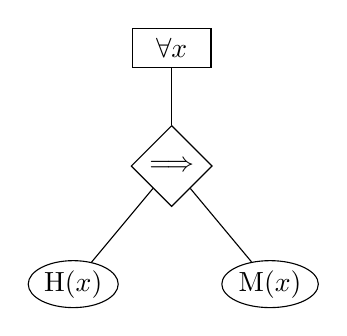
\begin{tikzpicture}[syntree]
        \node[quantifier] {{\(\forall x\)}}
            child { node[connective] {\(\implies\)} 
              child { node[literal] {\(\text{H}(x)\)} }
              child { node[literal] {\(\text{M}(x)\)} }
            };
    \end{tikzpicture}
    \caption{Syntactic tree for \(\forall x (\text{H}(x) \implies \text{M}(x))\)}\label{fig:syntactic_tree}
\end{figure}

In this representation, it is possible to omit the parentheses around the subformulae, as the tree structure already encodes the necessary grouping.

Moreover, is possible to isolate a \emph{subgrammar} by considering only the rules that generate atomic formulae (excluding so the ones deriving from \(\phi\)). Doing this easily allows to define the concept of \textbf{subterm} as a \emph{proper subtree} of the syntactic tree that represents an atomic formula (or by extension a literal).

An example of such a tree is shown in Figure~\ref{fig:subterm_tree} for the atomic formula \(P(f(x, g(y)))\).
\begin{figure}[H]
    \centering
    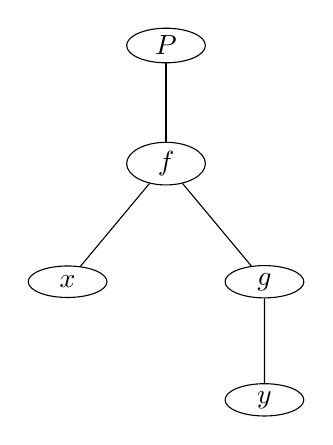
\begin{tikzpicture}[syntree]
        \node[literal] {\(P\)}
            child { node[literal] {\(f\)}
              child { node[literal] {\(x\)} }
              child { node[literal] {\(g\)}
                child { node[literal] {\(y\)} }
              }
            };
    \end{tikzpicture}
    \caption{Syntactic tree for the atomic formula \(P(f(x, g(y)))\) showing nested function structure}\label{fig:subterm_tree}
\end{figure}

If we consider multiple atomic formulae (or literals), is possible to represent them as a \textbf{forest} of syntactic trees, where each tree represents an atomic formula.

\begin{figure}[H]
    \centering
    \begin{minipage}[t]{0.48\textwidth}
        \centering
        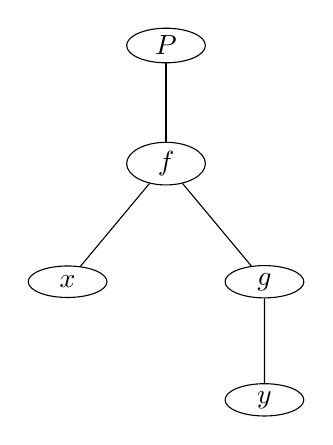
\begin{tikzpicture}[syntree]
            \node[literal] {\(P\)}
                child { node[literal] {\(f\)}
                  child { node[literal] {\(x\)} }
                  child { node[literal] {\(g\)}
                    child { node[literal] {\(y\)} }
                  }
                };
        \end{tikzpicture}
    \end{minipage}
    \hfill
    \begin{minipage}[t]{0.48\textwidth}
        \centering
        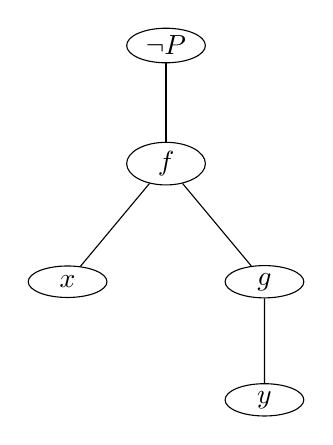
\begin{tikzpicture}[syntree]
            \node[literal] {\(\neg P\)}
                  child { node[literal] {\(f\)}
                    child { node[literal] {\(x\)} }
                    child { node[literal] {\(g\)}
                      child { node[literal] {\(y\)} }
                    }
                  };
        \end{tikzpicture}
    \end{minipage}
    \caption{Forest of the literals \(P(f(x, g(y)))\) and \(\neg P(f(x, g(y)))\)}\label{fig:subterm_forest}
\end{figure}

% Add a line to introduce DAG representation and explain why in practice it's better
In practice, it is often more convenient to represent these structures as Directed Acyclic Graphs (DAGs) rather than trees. This is because DAGs allow for the sharing of subterms, which can lead to more compact representations and easier manipulation of the formulae.

DAGs can be particularly useful in automated reasoning and theorem proving, where the same subterm may appear in multiple places within a formula. By representing the formula as a DAG, we can avoid redundant copies of the subterms and simplify the reasoning process.

\begin{figure}[H]
    \centering
    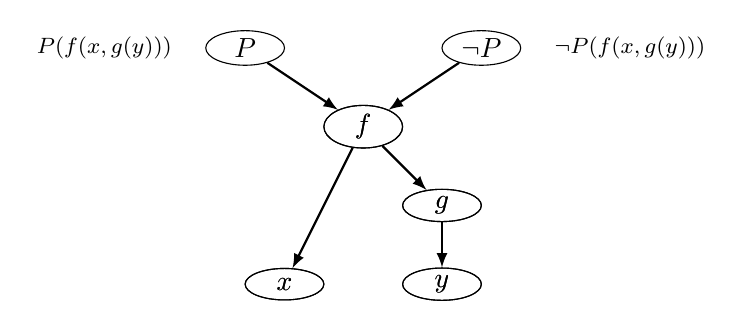
\begin{tikzpicture}[syntree]
        % Livello delle variabili (condivise)
        \node[literal] (x) at (0,0) {\(x\)};
        \node[literal] (y) at (2,0) {\(y\)};
        
        % Livello delle funzioni (condivise)
        \node[literal] (g) at (2,1) {\(g\)};
        \node[literal] (f) at (1,2) {\(f\)};
        
        % Livello dei predicati (separati)
        \node[literal] (P_pos) at (-0.5,3) {\(P\)};
        \node[literal] (P_neg) at (2.5,3) {\(\neg P\)};
        
        % Connessioni condivise
        \draw[-latex, thick] (g) -- (y);
        \draw[-latex, thick] (f) -- (x);
        \draw[-latex, thick] (f) -- (g);

        % Connessioni per literal positivo
        \draw[-latex, thick] (P_pos) -- (f);

        % Connessioni per literal negativo
        \draw[-latex, thick] (P_neg) -- (f);


        % Etichette
        \node[left=0.3cm of P_pos, font=\footnotesize] {\(P(f(x, g(y)))\)};
        \node[right=0.3cm of P_neg, font=\footnotesize] {\(\neg P(f(x, g(y)))\)};
        
        % Evidenzia i nodi condivisi con colore diverso
        \node[literal] at (x) {\(x\)};
        \node[literal] at (y) {\(y\)};
        \node[literal] at (g) {\(g\)};
        \node[literal] at (f) {\(f\)};
    \end{tikzpicture}
    \caption{DAG representation showing shared subterms between \(P(f(x, g(y)))\) and \(\neg P(f(x, g(y)))\)}\label{fig:subterm_dag}
\end{figure}

\subsection{Semantics}\label{subsec:semantics}

To formalize semantics in FOL, we need to define the meaning of the symbols and the truth conditions for the formulae. This is typically done using a \emph{model}, which consists of a domain of discourse and an interpretation function that assigns meanings to the constants, functions, and predicates.

A \textbf{model} for a FOL language is a pair \(M = (D, I)\), where:
\begin{itemize}
  \item \(D\) is a non-empty set, called the \textbf{domain of discourse}.
  \item \(I\) is an interpretation function that assigns:
  \begin{itemize}
    \item Each constant \(c \in \mathcal{C}\) to an element \(I(c) \in D\).
    \item Each function symbol \(f \in \mathcal{F}\) to a function \(I(f): D^{n_f} \to D\), where \(n_f\) is the arity of \(f\).
    \item Each predicate symbol \(P \in \mathcal{P}\) to a relation \(I(P) \subseteq D^{n_P}\), where \(n_P\) is the arity of \(P\).
  \end{itemize}
\end{itemize}

The truth value of a formula \(\phi\) in a model \(M\) is determined by the interpretation function and the structure of the formula as follows:

\subsubsection{Variable Assignment}\label{subsubsec:variable_assignment}
Given a model \(M = (D, I)\), a \textbf{variable assignment} (or \textbf{valuation}) is a function \(\sigma: \mathcal{V} \to D\) that assigns each variable to an element of the domain. We denote by \(\sigma[x \mapsto d]\) the assignment that is identical to \(\sigma\) except that it maps variable \(x\) to element \(d \in D\).

\subsubsection{Term Evaluation}
The \textbf{evaluation} of a term \(t\) in model \(M\) under assignment \(\sigma\), denoted \(\llbracket t \rrbracket_M^\sigma\), is defined recursively:
\begin{itemize}
  \item If \(t\) is a variable \(x\), then \(\llbracket x \rrbracket_M^\sigma = \sigma(x)\).
  \item If \(t\) is a constant \(c\), then \(\llbracket c \rrbracket_M^\sigma = I(c)\).
  \item If \(t = f(t_1, \ldots, t_n)\) where \(f\) is an \(n\)-ary function symbol, then 
        \[\llbracket f(t_1, \ldots, t_n) \rrbracket_M^\sigma = I(f)(\llbracket t_1 \rrbracket_M^\sigma, \ldots, \llbracket t_n \rrbracket_M^\sigma)\]
\end{itemize}

\subsubsection{Truth Conditions}
The \textbf{satisfaction} of a formula \(\phi\) in model \(M\) under assignment \(\sigma\), denoted \(M, \sigma \models \phi\), is defined recursively:

\begin{itemize}
  \item \textbf{Atomic formulae:}
  \begin{itemize}
    \item \(M, \sigma \models P(t_1, \ldots, t_n) \leftrightarrow (\llbracket t_1 \rrbracket_M^\sigma, \ldots, \llbracket t_n \rrbracket_M^\sigma) \in I(P)\)
    \item \(M, \sigma \models \top\) (always true)
    \item \(M, \sigma \not\models \bot\) (never true)
  \end{itemize}
  
  \item \textbf{Logical connectives:}
  \begin{itemize}
    \item \(M, \sigma \models \neg \phi \leftrightarrow M, \sigma \not\models \phi\)
    \item \(M, \sigma \models \phi \land \psi \leftrightarrow M, \sigma \models \phi\) and \(M, \sigma \models \psi\)
    \item \(M, \sigma \models \phi \lor \psi \leftrightarrow M, \sigma \models \phi\) or \(M, \sigma \models \psi\)
    \item \(M, \sigma \models \phi \implies \psi \leftrightarrow M, \sigma \not\models \phi\) or \(M, \sigma \models \psi\)
    \item \(M, \sigma \models \phi \iff \psi \leftrightarrow \left(M, \sigma \models \phi \text{ and } M, \sigma \models \psi\right) \text{ or } \left(M, \sigma \not\models \phi \text{ and } M, \sigma \not\models \psi\right)\)
  \end{itemize}
  
  \item \textbf{Quantifiers:}
  \begin{itemize}
    \item \(M, \sigma \models \forall x  \ms  \phi\) if and only if for all \(d \in D\), \(M, \sigma[x \mapsto d] \models \phi\)
    \item \(M, \sigma \models \exists x  \ms  \phi\) if and only if there exists some \(d \in D\) such that \(M, \sigma[x \mapsto d] \models \phi\)
  \end{itemize}
\end{itemize}

\subsubsection{Semantic Notions}
A formula \(\phi\) is:
\begin{itemize}
  \item \textbf{Satisfiable} if there exists a model \(M\) and assignment \(\sigma\) such that \(M, \sigma \models \phi\).
  \item \textbf{Valid} (sometimes called a \textbf{tautology}) if for all models \(M\) and assignments \(\sigma\), \(M, \sigma \models \phi\). We write \(\models \phi\).
  \item \textbf{Unsatisfiable} (or \textbf{contradictory}) if for all models \(M\) and assignments \(\sigma\), \(M, \sigma \not\models \phi\).
\end{itemize}

For a set of formulae \(\Gamma\) and a formula \(\phi\), we say \(\Gamma\) \textbf{semantically entails} \(\phi\), written \(\Gamma \models \phi\), if for all models \(M\) and assignments \(\sigma\):
  \[\text{if } M, \sigma \models \psi \text{ for all } \psi \in \Gamma, \text{ then } M, \sigma \models \phi\]

It is worth noticing that satisfiability and validity are closely related:
\begin{theorem}[Validity-Satisfiability Reduction]\label{thm:validity_satisfiability_reduction}
A formula \(\phi\) is valid if and only if \(\neg\phi\) is unsatisfiable. Formally:
\[\models \phi \iff \neg\phi \text{ is unsatisfiable}\]
\end{theorem}

\begin{proof}[Proof Sketch]
To prove this theorem, we need to show both directions of the equivalence.
  \begin{description}
    \item[(\(\Rightarrow\))] If \(\phi\) is valid, then \(M, \sigma \models \phi\) for all models \(M\) and assignments \(\sigma\). Therefore, \(M, \sigma \not\models \neg\phi\) for all \(M, \sigma\), making \(\neg\phi\) unsatisfiable.
    \item[(\(\Leftarrow\))] If \(\neg\phi\) is unsatisfiable, then there is no model \(M\) and assignment \(\sigma\) such that \(M, \sigma \models \neg\phi\). Therefore, for all \(M, \sigma\), we have \(M, \sigma \models \phi\), making \(\phi\) valid.
  \end{description}
\end{proof}


\section{Substitutions and Unification}
In Section~\ref{subsubsec:variable_assignment} we introduced the notation \(\sigma[x \mapsto d]\) to indicate a variable assignment in the semantic evaluation of a formula. We now extend this concept to the purely \emph{syntactic} setting, where variables are replaced by \emph{terms} rather than by elements of the interpretation domain. This leads to the notions of \emph{substitution}, \emph{unification}, and \emph{most general unifier}.

\subsection{Substitutions}
Given a term or literal \(\tau\), the notation \(\tau[x_k \mapsto t]\) denotes the expression obtained by replacing every occurrence of the variable \(x_k\) in \(\tau\) with the term \(t\).  
For example, if \(\tau = g(x_1, x_2)\), then:
\begin{equation}
\tau[x_1 \mapsto h] = g(h, x_2)
\end{equation}

A \textbf{substitution} is a function mapping a subset of variables \(\mathcal{V}^{'} \subseteq \mathcal{V}\) to a set of terms \(\mathcal{T} \subseteq \mathcal{V} \cup \mathcal{F} \cup \mathcal{C}\):
\begin{equation}
\sigma = \{ (x_1, t_1), \ldots, (x_n, t_n) \}
\end{equation}
If \(\tau\) is a term and \(\sigma\) is a substitution, we write \(\tau\sigma\) or \(\tau[x_1 \mapsto t_1, \ldots, x_n \mapsto t_n]\) for the term obtained by replacing all \(x_i\) with \(t_i\) \emph{simultaneously}.  
The word “simultaneously” means that each replacement is made with respect to the \emph{original} \(\tau\), without the effect of one replacement influencing another.

For instance, if \(\tau = f(x_1, x_2)\), then:
\begin{equation}
\tau[x_1 \mapsto x_2,  \ms  x_2 \mapsto x_1] = f(x_2, x_1)
\end{equation}
and not \(f(x_1, x_1)\), which would arise from sequential application.

\subsection{Generality of  Substitutions}
For two substitutions \(\sigma_1\) and \(\sigma_2\), we say \(\sigma_1\) is \textbf{more general} than \(\sigma_2\) if for every term \(\tau\) there exists a substitution \(\theta\) such that:
\begin{equation}  
  \tau\sigma_2 = (\tau\sigma_1)\theta
\end{equation}

If there is a substitution \(\sigma\) with:
\begin{equation}
\tau_1\sigma = \tau_2\sigma
\end{equation}
then \(\tau_1\) and \(\tau_2\) are said to be \textbf{unifiable}, and \(\sigma\) is called a \textbf{unifier}.

A unifier \(\sigma\) for two terms \(\tau_1\) and \(\tau_2\) is called a \textbf{most general unifier} (MGU) if it is more general than any other unifier of \(\tau_1\) and \(\tau_2\).

\subsection{Unification Beyond Single Terms}
The unification concept extends to sets of terms, literals, and sets of literals.  
A set of terms \(\mathcal{T}\) is \textbf{unifiable} if there exists a substitution \(\sigma\) such that for any \(\tau_i, \tau_j \in \mathcal{T}\) we have \(\tau_i\sigma = \tau_j\sigma\). In this case, \(\sigma\) is a unifier of \(T\).

Two literals with the same arity:
\begin{equation}
L_1 = P(\tau_1, \ldots, \tau_n), \quad L_2 = \neg P(\tau'_1, \ldots, \tau'_n)
\end{equation}
are unifiable if there is a substitution making them identical, disregarding negation. Equivalently, if \(f\) is a fresh \(n\)-ary function symbol, then \(L_1\) and \(L_2\) are unifiable if and only if \(f(\tau_1, \ldots, \tau_n)\) and \(f(\tau'_1, \ldots, \tau'_n)\) are unifiable.  
Literals of different arities are never unifiable.

\subsection{Obstructions to Unification}
When attempting to unify two terms, two main forms of obstruction can occur:
\begin{enumerate}
    \item \textbf{Function obstruction:} in a parallel traversal of the syntactic trees of both terms, two different function symbols occur at corresponding positions. For example:
    \[
    f(x_1, g_1(x_2)) \quad\text{and}\quad f(x_1, g_2(x_2))
    \]
    are not unifiable because \(g_1 \neq g_2\).
    \item \textbf{Variable obstruction:} in a parallel traversal, a variable \(x\) appears in one term while the other term contains a subterm \(t \neq x\) in which \(x\) occurs. For example:
    \[
    h(x_1, k(x_2)) \quad\text{and}\quad h(k(x_1), x_1)
    \]
    are not unifiable because \(x_1\) occurs inside \(k(x_1)\).
\end{enumerate}

In general so, if two terms are not unifiable, then at least one of the following holds:
\begin{enumerate}
    \item The terms have different arities.
    \item The terms exhibit a function obstruction.
    \item The terms exhibit a variable obstruction.
\end{enumerate}


\subsection{Complexity of Unification}
The computational complexity of unification has been extensively studied since the 1960s.
Early approaches exhibited worst-case exponential behaviour due to the difficulty of detecting variable obstructions efficiently~\cite{robinson1965}.
However, significant theoretical advances in the 1970s led to the development of linear-time unification algorithms that achieve \(O(n)\) complexity, where \(n\) is the combined size of the input terms~\cite{martelli1976, paterson1978}.

These linear-time bounds represent optimal complexity for the unification problem, as any algorithm must examine all symbols in the input terms at least once.
Modern implementations incorporate various optimization techniques such as term indexing and specialized handling for common cases to improve average-case performance~\cite{baader2001}.
The unification problem belongs to complexity class \textbf{P}, making it tractable for practical applications in automated reasoning and logic programming systems.


\section{Skolemization and Normalization}

Often times, First-Order formulae undergo a series of transformations to prepare them for automated reasoning tasks.
These transformations include renaming variables, converting to normal forms, and Skolemization.
Raw first-order logic formulae, as naturally expressed, are typically not in a form that automated theorem provers and inference engines can efficiently process.
The transformation process standardizes the syntactic structure of formulae, eliminates certain logical constructs that complicate automated reasoning, and converts them into canonical forms that enable the systematic application of inference rules and resolution procedures.

\subsection{Negated Normal Form}
The first transformation applied is to convert the formula into \textbf{negated normal form} (NNF).

A formula is in NNF if it is described by the following CFG\@:
\begin{equation}
  \nu \to \top  \ms | \ms  \bot  \ms | \ms  L  \ms | \ms  \nu \land \nu  \ms | \ms  \nu \lor \nu  \ms | \ms  \forall x  \ms  \nu  \ms | \ms  \exists x  \ms  \nu \quad\quad \text{where } L \text{is a literal}
\end{equation}
where \(L\) is a \emph{literal}, that is defined as an atomic formula or its negation.
In a practical sense, NNF transformation involves pushing negations inward and eliminating implications and biconditionals.
In fact, every formula can be brought into this form by replacing implications (\(\implies\)) and equivalences (\(\iff\)) by their definitions, using De Morgan's laws to push negation inwards, and eliminating double negations. This process can be represented using the following rewrite rules:

\begin{equation}
  \begin{aligned}
    \phi \implies \psi &\leadsto \neg \phi \lor \psi \\
    \phi \iff \psi &\leadsto (\neg \phi \lor \psi) \land (\phi \lor \neg \psi) \\
    \neg (\phi \lor \psi) &\leadsto \neg \phi \land \neg \psi \\
    \neg (\phi \land \psi) &\leadsto \neg \phi \lor \neg \psi \\
    \neg \neg \phi &\leadsto \phi \\
    \neg \exists x  \ms  \phi &\leadsto \forall x  \ms  \neg \phi \\
    \neg \forall x  \ms  \phi &\leadsto \exists x  \ms  \neg \phi
  \end{aligned}
\end{equation}

The NNF version of a formula is \emph{equivalent} to the original formula, meaning they have the same truth value in every model.

\subsection{Skolemization}
In the context of automated reasoning, \textbf{Skolemization} is the process of eliminating existential quantifiers from a formula by introducing new symbols called \textbf{Skolem functions} or \textbf{Skolem constants}~\cite{skolem1920}.  
The result of Skolemization is not logically equivalent to the original formula, but it is \textbf{equisatisfiable}: both formulae are satisfiable in exactly the same set of interpretations.
The process of Skolemization goes as follows:

Let \(\phi\) be a formula in NNF\@. For every existential quantifier \(\exists x_k\) in \(\phi\):
\begin{itemize}
  \item If \(x_k\) is not in the scope of any universal quantifier, replace it with a new constant symbol \(c\) (a \emph{Skolem constant}).
  \item If \(x_k\) is in the scope of universal quantifiers over variables \(y_1, \dots, y_m\), replace \(x_k\) with a new function symbol \(f(y_1, \dots, y_m)\) (a \emph{Skolem function}) of arity \(m\), where \(y_1, \dots, y_m\) are all the universally quantified variables whose quantifiers appear in positions that bind variables free in the scope of \(\exists x_k\).
\end{itemize}
All Skolem symbols introduced must be fresh, i.e., not present in the original signature.


An example of this process is as follows:

Consider the formula:
\[
\forall x \: \exists y \: P(x, y)
\]
Since \(y\) is existentially quantified within the scope of \(\forall x\), we introduce a Skolem function \(f(x)\):
\[
\forall x \: P(x, f(x))
\]

The Skolemization process fundamentally transforms the logical structure of a formula while preserving its essential satisfiability characteristics.
Most notably, it completely eliminates all existential quantifiers from the formula, replacing them with concrete function or constant symbols that capture the dependencies between variables.
This transformation is particularly valuable because it preserves satisfiability—meaning that the original formula has a model if and only if the Skolemized version does—but it does not preserve validity in the reverse direction.
A formula that is valid before Skolemization may lose this property afterward, since the introduction of Skolem functions can create additional constraints that weren't present in the original formula.
However, the resulting formula contains only universal quantifiers, which significantly simplifies the reasoning process by enabling purely universal reasoning techniques. 
This uniform quantifier structure is especially advantageous for automated theorem provers, as it eliminates the need to handle the complex interactions between universal and existential quantifiers during proof search.

\subsection{Clausal Normal Form (CNF).}
A formula is in CNF if it is a conjunction of one or more \textbf{clauses}, each clause being a disjunction of literals.  
As NNF, CNF can be described by a CFG too:
\begin{equation}
  \begin{aligned}
    CNF &\to D  \ms | \ms  D \land CNF \\
      D &\to L  \ms | \ms  L \lor D
  \end{aligned}
\end{equation}
where \(L\) is a literal.

Every NNF formula, after undergoing Skolemization, can be transformed into CNF by applying \(\land\) and \(\lor\) distribution rules and dropping universal quantifiers.
Often, CNF formulae are represented as sets of clauses with the following notation:
\[
(A \lor B) \land (C \lor D) \equiv \{\{A , B\} \ms , \ms \{C , D\}\}
\]

As an example of the full pipeline of the transformation from general formula to CNF, for the formula \( \forall x  \ms \big( \ms (\exists y  \ms   P(x,y)) \leftrightarrow Q(x)  \ms  \big)\)
is the following:
\begin{enumerate}
    \item \textbf{Convert to NNF:}
    \begin{itemize}
        \item Eliminate \(\iff\):
          \[\forall x  \ms \big( (\neg \exists y_1 \ms  P(x,y_1) \lor Q(x)) \land (\neg Q(x) \lor \exists y_2 \ms  P(x,y_2))\big)\]
        \item Push negation inward using De Morgan's laws and quantifier duality:
    \end{itemize}
    \[
    \forall x \ms \Big(\big(\forall y \ms \neg P(x,y)\ \lor\ Q(x)\big)\ \land\ \big(\neg Q(x)\ \lor\ \exists y \ms  P(x,y)\big)\Big)
    \]
    
    
    \item \textbf{Skolemization:}
    \begin{itemize}
        \item Replace \(\exists y\) (in scope of \(\forall x\)) with Skolem function \(f(x)\):
    \end{itemize}
    \[
      \forall x \ms \Big(\big(\forall y \ms \neg P(x,y)\ \lor\ Q(x)\big)\ \land\ \big(\neg Q(x)\ \lor\ P(x,f(x))\big)\Big)
    \]
    \\
    \item \textbf{Convert to CNF:}
    \begin{itemize}
    \item Move all universal quantifiers to the front:
    \[
      \forall x \ms  \forall y \ms  \Big(\big(\neg P(x,y)\ \lor\ Q(x)\big)\ \land\ \big(\neg Q(x)\ \lor\ P(x,f(x))\big)\Big)
    \]
    \item Drop universal quantifiers and write as set of clauses:
    \[
      \{\{\neg P(x,y), Q(x)\}, \ms  \{\neg Q(x), P(x,f(x))\}\}
    \]
    \end{itemize}
    
\end{enumerate}

\begin{figure}[H]
  \centering
  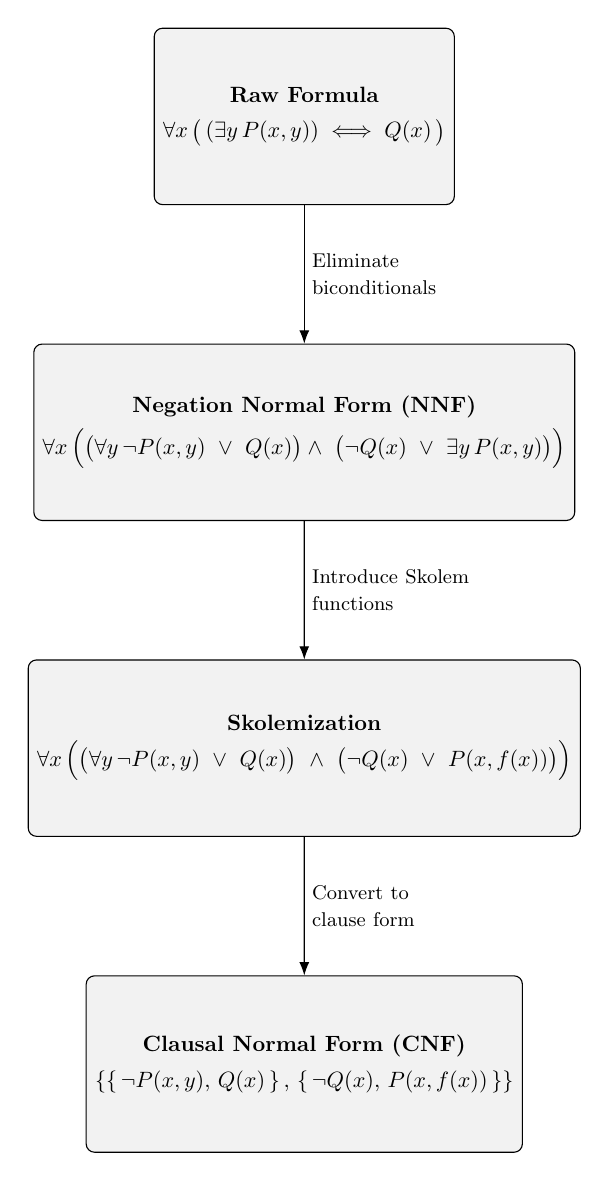
\begin{tikzpicture}[
      scale=0.8, % <-- SCALING FACTOR
      transform shape, % <-- ENSURE NODES AND TEXT ARE SCALED
      node distance=2.2cm and 0.8cm,
      stage/.style={draw, rounded corners=3pt, fill=gray!10, align=center, inner sep=4pt, minimum height=2.8cm},
      >=Latex
    ]

    % Nodes arranged vertically for better readability
    \node[stage] (raw) {\textbf{Raw Formula} \\[4pt]
      \(\displaystyle \forall x \ms \big( \ms (\exists y \ms  P(x,y)) \iff Q(x) \ms \big)\)};

    \node[stage, below=of raw] (nnf) {\textbf{Negation Normal Form (NNF)}\\[4pt]
      \(\displaystyle \forall x \ms \Big(\big(\forall y \ms \neg P(x,y)\ \lor\ Q(x)\big) \land\ \big(\neg Q(x)\ \lor\ \exists y \ms  P(x,y)\big)\Big)\)};


    \node[stage, below=of nnf] (sko) {\textbf{Skolemization}\\[4pt]
      \(\displaystyle \forall x \ms \Big(\big(\forall y \ms \neg P(x,y)\ \lor\ Q(x)\big)\ \land\ \big(\neg Q(x)\ \lor\ P(x,f(x))\big)\Big)\)};

    \node[stage, below=of sko] (cnf) {\textbf{Clausal Normal Form (CNF)}\\[4pt]
      \(\{\{ \ms \neg P(x,y), \ms  Q(x) \ms \} \ms , \ms \{ \ms \neg Q(x), \ms  P(x,f(x)) \ms \}\}\)};

    % Arrows
    \draw[->] (raw) -- node[right, text width=3cm, align=left]{\small Eliminate\\biconditionals} (nnf);
    \draw[->] (nnf) -- node[right, text width=3cm, align=left]{\small Introduce Skolem\\functions} (sko);
    \draw[->] (sko) -- node[right, text width=3cm, align=left]{\small Convert to\\clause form} (cnf);

  \end{tikzpicture}
  \caption{Clausification: Raw formula \(\rightarrow\) NNF  \(\rightarrow\) Skolemization \(\rightarrow\) CNF.}\label{fig:nnf-to-cnf-pipeline}
\end{figure}


Transforming formulae into CNF is a prerequisite for many automated reasoning techniques, particularly \emph{resolution}~\cite{chang1997}.  
By ensuring that the input is in a uniform syntactic format, inference rules can be applied in a purely mechanical way without further structural transformations.

This pipeline of transformations, combined with \emph{naming}, is also called \textbf{clausification} and  constitutes the \textbf{preprocessing} phase of automated reasoning systems, a crucial step to prepare formulae for \emph{inferences}.

\section{Auxiliary Predicate Introduction}

In the transformation of first-order logic (FOL) formulas, particularly when converting to clausal form, it is often advantageous to introduce \emph{auxiliary predicates} to represent complex subformulae. The general idea is to replace a subformula \(\psi(\bar{x})\) with\footnote{Here the notation \(\bar{x}\) is used as usual to indicate a sequence of variables} a fresh predicate symbol \(P(\bar{x})\) that does not occur in the original vocabulary, and to accompany this replacement with a \emph{defining axiom} of the form
\[
\forall \bar{x}\ \big(P(\bar{x}) \iff \psi(\bar{x})\big).
\]
This method is referred to in the literature under various names, including \emph{auxiliary predicate introduction}, \emph{definition introduction}, and, in some contexts, \emph{axiomatization}. The defining axiom ensures that \(P\) is logically equivalent to the original subformula, thereby preserving satisfiability and logical consequence.

One of the main motivations for this technique in automated theorem proving is the avoidance of an exponential increase in formula size during \emph{clausification}.
A naïve elimination of biconditionals and the distribution of disjunctions over conjunctions can lead to a number of clauses that grows exponentially with the size of the input.
By introducing auxiliary predicates for large or deeply nested subformulae, the number of resulting clauses can be kept proportional to the size of the original formula.

Another important application arises in the context of syntactically restricted fragments of FOL, such as the \emph{guarded fragment} or the \emph{fluted fragment}.
In these fragments, unrestricted formula transformations may produce formulas that fall outside the fragment, thereby forfeiting desirable properties such as decidability or favourable complexity bounds.
Here, auxiliary predicate introduction serves as a \emph{structure-preserving} transformation: rather than expanding a subformula in a way that would violate syntactic restrictions, a fresh predicate is introduced, with a defining axiom that maintains semantic equivalence while preserving the fragment membership of the formula.

\subsection{Polarity of Subformulae}

The concept of \emph{polarity} provides a finer-grained analysis of where and how a subformula occurs within a larger formula.
Intuitively, polarity describes whether an occurrence of a subformula is in a \emph{positive}, \emph{negative}, or \emph{neutral} position.
A subformula occurs positively if it is under the scope of an even number of negations, and negatively if it is under the scope of an odd number of negations.
The \emph{neutral} (or \emph{zero}) polarity occurs in positions where a subformula is required in both directions of entailment, most notably when it appears under a biconditional, where neither purely positive nor purely negative reasoning suffices.

Polarity is defined inductively as follows:
\[
\begin{aligned}
&\text{(Base case)} && \mathrm{pol}(\varphi) = + \quad \text{if } \varphi \text{ is the whole formula}, \\[2pt]
&\text{(Negation)} && \mathrm{pol}(\neg \varphi) = -\mathrm{pol}(\varphi), \\[2pt]
&\text{(Conjunction / Disjunction)} && 
\begin{cases}
\mathrm{pol}(\varphi) = \mathrm{pol}(\varphi \landor \psi), \\
\mathrm{pol}(\psi) = \mathrm{pol}(\varphi \landor \psi),
\end{cases} \\[4pt]
&\text{(Implication)} && 
\begin{cases}
\mathrm{pol}(\varphi) = -\mathrm{pol}(\varphi \rightarrow \psi), \\
\mathrm{pol}(\psi) = \mathrm{pol}(\varphi \rightarrow \psi),
\end{cases} \\[4pt]
&\text{(Biconditional)} && 
\begin{cases}
\mathrm{pol}(\varphi) = 0, \\
\mathrm{pol}(\psi) = 0,
\end{cases} \quad \text{for } \varphi \leftrightarrow \psi \text{ with any polarity}, \\[4pt]
&\text{(Quantifiers)} && \mathrm{pol}(\varphi) = \mathrm{pol}(\mathcal{Q} x\, \varphi), \quad \mathcal{Q} \in \{\forall, \exists\}.
\end{aligned}
\]
Here, \(+\) denotes positive polarity, \(-\) denotes negative polarity, and \(0\) denotes neutral polarity.



\subsection{Polarity-Aware Auxiliary Predicate Introduction}

Polarity analysis allows for an optimization of auxiliary predicate introduction. If a subformula \(\psi(\bar{x})\) occurs only positively in the formula, it is sufficient to introduce the fresh predicate \(P(\bar{x})\) together with the implication
\[
\forall \bar{x}\ \big(P(\bar{x}) \rightarrow \psi(\bar{x})\big),
\]
rather than the full biconditional. Conversely, if \(\psi(\bar{x})\) occurs only negatively, it suffices to add
\[
\forall \bar{x}\ \big(\psi(\bar{x}) \rightarrow P(\bar{x})\big).
\]
The full biconditional is necessary only when \(\psi(\bar{x})\) occurs with zero polarity.

This optimization is widely used in \emph{definitional CNF transformations} for first-order theorem proving. By introducing only the necessary direction of the equivalence, the number of clauses generated during clausification can be reduced, often substantially, while still preserving the correctness of the transformation with respect to satisfiability and logical consequence.









    \chapter{Inference systems}\label{chap:inference-systems}

In chapter~\ref{chap:first-order-logic} we introduced FOL as a formal representation of knowledge, and we discussed its syntax and semantics.
Representation of knowledge alone is not sufficient for formalizing reasoning processes.
What is needed is a formalization of some reasoning mechanisms that can operate on this knowledge, rules that, given a set of premises, can derive new conclusions.

These rules are called \textbf{inference rules}.
There are various types of inference rules, each with its own characteristics and applications.

In general, we denote with \(R\) a set of inference rules called \textbf{inference system}. Given a set of premises \(\Gamma\), an inference rule \(r \in R\) can be applied to \(\Gamma\) to infer a new conclusion \(\phi\), denoted as \(\Gamma \vdash_r \phi\)\footnote{
  The notation can be simplified with just \(\Gamma \vdash \phi\) if the specific rule \(r\) is unambiguous.}.
If a sentence \(\phi\) can be inferred from the empty set using \(r\), we write \(\vdash_r \phi\).
It is possible to generalize this notation to the entire inference system \(R\) by writing \(\Gamma \vdash_{R} \phi\).

Moreover, it is possible to characterize the effectiveness of inference systems with various properties:

\begin{itemize}
    \item \textbf{Soundness}: An inference system is sound if it only derives conclusions that are true in the model. Formally, \(R\) is \textbf{sound} if for all \(\Gamma\) and \(\phi\), if \(\Gamma \vdash_{R} \phi\), then \(\Gamma\models\phi\).
    \item \textbf{Completeness}: An inference system is complete if it can derive all conclusions that are true in the model. Formally, \(R\) is \textbf{complete} if for all \(\Gamma\) and \(\phi\), if \(\Gamma\models\phi\), then \(\Gamma \vdash_{R} \phi\).
    \item \textbf{Correctness}: An inference system is correct if it is both \textbf{sound} and \textbf{complete}.
    \item \textbf{Consistency}: An inference system is consistent if it does not derive contradictory conclusions from any set of premises. Formally, \(R\) is \textbf{consistent} if for all \(\Gamma\) and \(\phi\), it is not the case that both \(\Gamma \vdash_{R} \phi\) and \(\Gamma \vdash_{R} \neg \phi\).
\end{itemize}
A weaker form of completeness is \textbf{refutational completeness} which requires that if \(\Gamma \models \bot\), then \(\Gamma \vdash_{R} \bot\).  Practically, this means that if a set of premises is unsatisfiable, the inference system can derive a contradiction.
By theorem~\ref{thm:validity_satisfiability_reduction}, a refutational complete inference system can show that a formula is valid by proving that its negation is unsatisfiable.

A first example of an inference rule is \textbf{Modus Ponens}, which states that if we have a conditional statement \(A \implies B\), and we know that \(A\) is true, then we can conclude that \(B\) is also true. Formally, it can be expressed as:
\begin{equation}  
  \infer{B}{A & A \implies B}
\end{equation}


Or, alternatively, and more conveniently for formulae in CNF, we can express it as:
\begin{equation}  
  \infer{B}{A & \neg A \lor B}
\end{equation}

A classical application of Modus Ponens can be found in Aristotelian syllogisms, where we have two premises and a conclusion.
An example of a syllogism is:
\begin{quote}
  All humans are mortal. Socrates is a human. Therefore, Socrates is mortal.
\end{quote}
The premises can be formalized as:
\begin{equation}
  \forall x \ms H(x) \implies M(x), \qquad H(s)
\end{equation}
These can be converted into CNF as:
\begin{equation}
    \neg H(x) \lor M(x), \qquad H(s)
\end{equation}

In FOL, before applying Modus Ponens, we must ensure that the premises contain a matching literal. To do this, we need to find the MGU \(\sigma\) that makes the literals match that, in this case, is \(\sigma = \{(x,s)\}\).
Finally, we can apply Modus Ponens for deriving the conclusion \(M(s)\) (Socrates is mortal) as follows:
\begin{equation}
  \infer{M(s)}{H(s) & \neg H(x) \lor M(x)}
\end{equation}

From this example, we can define a more specific form of Modus Ponens for FOL, which takes into account the need for matching literals and the use of MGUs.
\begin{equation}  
  \infer{B\sigma}{A_1 & A_2 \implies B} \qquad \text{or} \qquad \infer{B\sigma}{A_1 & \neg A_2 \lor B}
\end{equation}
where \(\sigma\) is the MGU of \(A_1\) and \(A_2\).

While being a powerful inference rule, Modus Ponens has its limitations in the context of FOL\@.
In particular:
\begin{itemize}
  \item It is \textbf{sound} because any conclusion derived is logically entailed.
  \item It is \textbf{not complete} because there are valid conclusions that cannot be derived using this rule alone.
  \item It is \textbf{not refutationally complete} because there are unsatisfiable sets of clauses that cannot be shown to be unsatisfiable using this rule alone.
\end{itemize}

For example, the set of clauses
\begin{equation}\label{eq:example_unsat}  
  \{\{\neg A, B\},\{\neg A , \neg B\}, \{\neg C , A\}, \{A , C\}\}
\end{equation}


This set is unsatisfiable:
\begin{description}
  \item[Assuming \(A\) true] From clause 1 we have \(B\) true, and from clause 2 we have \(\neg B\) true, leading to a contradiction.
  \item[Assuming \(A\) false] From clause 3 we have \(\neg C\) true, and from clause 4 we have \(C\) true, leading to a contradiction.
\end{description}
However, Modus Ponens alone cannot derive this contradiction because there are no atomic clauses to trigger the inference.

This limitation of Modus Ponens motivates the need for more general inference rules that can handle cases where no unit clauses are available to trigger inferences.
The resolution rule addresses this limitation by allowing inferences between any clauses containing complementary literals, regardless of their structure.

\section{Resolution and Factoring}

A common inference system used in FOL is based on the \textbf{resolution} rule, which allows for the derivation of new clauses from existing ones, with the addition of the \textbf{factoring} rule, that allows for the simplification of clauses by removing redundant literals.

The key insight is that Modus Ponens requires one premise to be a unit clause (single literal) to match against a conditional.
Resolution generalizes this by allowing any two clauses containing literals that become complementary after unification to be combined, making it much more powerful for systematic proof search in clause form.

\subsection{Resolution}

\textbf{Resolution} is a rule of inference specifically designed for CNF\@. It allows for the derivation of new clauses by resolving two clauses that contain complementary literals.

Formally, resolution in FOL can be defined as:

\begin{equation}
  \infer{(B\lor C)\sigma}{A_1 \lor B & \neg A_2 \lor C}
\end{equation}
\indent where \(\sigma\) is the MGU of \(A_1\) and \(A_2\).

\noindent Intuitively, resolution is justifiable noticing that, for \(A_1 \lor B\) and \(A_2 \lor C\) to be true, at least one of \(A_1\) and \(B\) must be true, and at least one of \(A_2\) and \(C\) must be true.
Being \(A_1\) and \(A_2\) complementary, it is impossible for both to be true at the same time, so at least one of \(B\) and \(C\) must be true. Thus, we can conclude that \(B \lor C\) must be true.

From this consideration, we can see that resolution is \textbf{sound} because it only derives conclusions that are logically entailed by the premises.
However, resolution is \textbf{not complete} because there are valid conclusions that cannot be derived using this rule alone.
An example of this is the \emph{disjunction introduction} rule \(A \models A \lor B\), which allows for the introduction of a disjunction from a single clause.

The absence of complementary literals in the premises prevents resolution from deriving any conclusions, and therefore to be complete.

Resolution though is \textbf{refutationally complete}, meaning that if a set of clauses is unsatisfiable, resolution can derive the empty clause (\citeauthor{robinson1965}\cite{robinson1965}), denoted \(\varnothing\), representing a contradiction --- a clause with no literals that can never be satisfied.
Using resolution, we can easily show that the previous example set of clauses~\ref{eq:example_unsat} is unsatisfiable:
\begin{equation}
  \begin{aligned}
    \neg A \lor B &\quad \text{Clause 1 (Premise)} \\
    \neg A \lor \neg B &\quad \text{Clause 2 (Premise)} \\
    \neg C \lor A &\quad \text{Clause 3 (Premise)} \\
    A \lor C &\quad \text{Clause 4 (Premise)} \\
    \neg A &\quad \text{Clause 5 (Resolution 1,2)} \\
    A &\quad \text{Clause 6 (Resolution 3,4)} \\
    \varnothing &\quad \text{Clause 7 (Resolution 5,6)}
  \end{aligned}
\end{equation}
\uninatodo{Not sure if this is the correct place for saturation algorithm. Maybe the vampire chapter is better suited?}
This can be achieved by a \textbf{saturation} process, where we repeatedly apply resolution to derive new clauses until either the empty clause is derived or no new clauses can be generated.

Formally, a set of clauses \(S\) is \textbf{saturated} under resolution if no new clauses can be derived by applying resolution to clauses in \(S\).
A possible implementation of a saturation algorithm is implemented partitioning the set of clauses into two collections: 

\begin{itemize}
  \item \textbf{active} clauses \(A\) that starts empty, where clauses are inserted after being resolved against the other clauses in the active set
  \item \textbf{passive} clauses \(P\) that starts containing all clauses in the original set \(S\), where clauses are removed one at a time as they are resolved, and new clauses obtained by resolution are inserted
\end{itemize}

When \(P\) becomes empty, we can conclude that the original set of clauses \(S\) is satisfiable, because all clauses have been resolved without deriving a contradiction.
If, instead, at any point we derive the empty clause, we can conclude that \(S\) is unsatisfiable.

A high-level description of the saturation algorithm is as follows:
\begin{algorithm}[H]
    \caption{Saturation Algorithm}\label{alg:padding}
    \begin{algorithmic}[1]
        \Statex{} \textbf{signature} \(\textsc{SA} \quad [Clause] \to Boolean\)
        \Statex{} \textbf{ensure} The returned CSA are box-compatible
        \Function{\(\textsc{SA}\)}{$S$} % chktex 46
            \State{} \((A,P)\gets (\emptyset,S)\)
            \While{\(P \neq \emptyset\)}
                \State{} \(curr \gets select(P)\)
                \State{} \(P \gets P \setminus \{curr\}\)
                \State{} \(New \gets \emptyset\)
                \ForAll{\(clause \in A\)} 
                    \State{} \(r \gets resolve(curr, clause)\)
                    \If{\(r \neq \varnothing\)}
                        \State{} \textbf{return} \(False\)
                    \ElsIf{\(r \neq \bot\)}
                        \State{} \(New \gets New \cup \{r\}\)
                    \EndIf{}
                \EndFor{}
                \State{} \(A \gets A \cup \{curr\}\)
                \State{} \(P \gets P \cup New\)
            \EndWhile{}
            \State{} \textbf{return} \(True\)
        \EndFunction{}
    \end{algorithmic}
\end{algorithm}

Where \(resolve\) is a function of type \(Clause \times Clause \to Clause\ms |\ms \bot\) that computes the resolvent of two clauses, or returns \(\bot\) if no matching literals can be found.

This algorithm explores the search space of all possible resolutions, systematically applying the resolution rule to derive new clauses until either a contradiction is found or no new clauses can be generated.
This function is \emph{partial}, because termination is not guaranteed in all cases.
An example of non-terminating input is the set of clauses
\begin{equation}\label{eq:non_terminating}
  \{ \{P(c)\}, \{\neg P(x) \lor P(f(x))\} \}
\end{equation}
which is satisfiable by \emph{Peano Arithmetic} (interpreting \(c\) as \(0\) and \(f\) as the successor function), but leads to an infinite loop in the saturation algorithm.

\begin{equation}
   \begin{aligned}
    P(c) &\quad \text{Clause 1 (Premise)} \\
    \neg P(x) \lor P(f(x)) &\quad \text{Clause 2 (Premise)} \\
    \neg P(f(c)) &\quad \text{Clause 3 (Resolution 1,2)} \\
    \neg P(f(f(c))) &\quad \text{Clause 4 (Resolution 3,2)} \\
    \neg P(f(f(f(c)))) &\quad \text{Clause 5 (Resolution 4,2)}\\
    \ldots
  \end{aligned}
\end{equation}

This limitation is not a deficiency of resolution itself, but rather reflects an intrinsic property of first-order logic. The undecidability of first-order logic was proven by \citeauthor{church1936}~\cite{church1936} and \citeauthor{turing1936}~\cite{turing1936} in 1936, showing that no algorithm can decide the validity (or satisfiability) of arbitrary first-order formulas.

Resolution is optimal in the sense that it achieves the best possible: it is a \textbf{semi-decision procedure} that will always find a proof when one exists, but may run indefinitely when no proof exists. This is the theoretical limit for any sound and complete inference system for first-order logic.

\subsection{Factoring}

In addition to resolution, \textbf{factoring} is a rule that allows for the simplification of clauses by removing redundant literals.
In contrast to the inference rules seen so far, factoring does not derive new conclusions but rather simplifies existing clauses, improving their efficiency in the proof search.

Formally, factoring can be defined as:
\begin{equation}
  \infer{(C \lor A_1)\sigma}{C \lor A_1 \lor A_2}
\end{equation}
\indent where \(\sigma\) is the MGU of \(A_1\) and \(A_2\).

\noindent Factoring eliminates duplicate literals that arise after unification. If a clause contains two literals that can be unified with MGU \(\sigma\), then applying \(\sigma\) would make them identical, and we can simplify using the tautology \(A \lor A \iff A\).

For example, from the clause \(P(x) \lor Q(y) \lor P(f(y))\), we can factor on \(P(x)\) and \(P(f(y))\) with MGU \(\sigma = \{(x , f(y))\}\) to get \((P(x) \lor Q(y))\sigma = P(f(y)) \lor Q(y)\).

While resolution alone is refutationally complete, factoring serves as an optimization that reduces clause size and prevents the search space from being cluttered with subsumed clauses. This can significantly improve the performance of resolution-based theorem provers.

For instance, without factoring, we might derive increasingly complex clauses when the simpler factored form would suffice for the same logical content.

\section{Ordered Inferences}

While resolution and factoring provide a refutationally complete inference system, unrestricted application of these rules can lead to an explosion of irrelevant clauses, severely impacting efficiency. The key insight is that many inferences are redundant or unnecessary for finding a refutation.

Ordered inference rules address this problem by imposing systematic restrictions on when resolution and factoring can be applied, dramatically reducing the search space while preserving refutational completeness.

\subsection{Admissible Ordering}

The foundation of ordered inferences is an \textbf{admissible ordering} on literals, which guides the selection of inference candidates.

An ordering \(\succ\) on literals is \textbf{admissible} if it satisfies:
\begin{itemize}
    \item \textbf{Well-foundedness and totality on ground literals}: for any two ground literals \(L_1\) and \(L_2\), either \(L_1 \succ L_2\), \(L_2 \succ L_1\), or \(L_1 = L_2\) (totality), and each subset of ground literals has a minimal element (well-foundedness).
    \item \textbf{Atom constraints}: for any atoms \(A\) and \(B\), it satisfies \(\neg A \succ A\) and \(B \succ A\) implies \(B \succ \neg A\).
    \item \textbf{Stability under substitution (Liftable)}: if \(L_1 \succ L_2\), then \(L_1\sigma \succ L_2\sigma\) for any substitution \(\sigma\)
\end{itemize}

Common examples of admissible orderings include lexicographic orderings on terms and literals, where terms are compared first by their structure (function symbols, arity) and then by their arguments recursively.

For instance, using a lexicographic ordering where \(f \succ g\) and \(a \succ b\):
\[f(a) \succ f(b) \succ g(a) \succ g(b) \succ a \succ b\]

The ordering extends to literals by considering both the predicate symbols and their arguments, considering the \emph{depth} of terms.

\subsection{Ordered Resolution}

\textbf{Ordered resolution} restricts the resolution rule to apply only when certain maximality conditions are satisfied.

Formally, ordered resolution can be defined as:

\begin{equation}
  \infer{(B\lor C)\sigma}{C\lor A_1 & \neg A_2 \lor B}
\end{equation}
  
\indent provided (i) \(\sigma\) is the MGU of \(A_1\) and \(A_2\), (ii) \(A_1\sigma\) is strictly maximal respect to \(B\sigma\), and \indent (iii) \(\neg A_2\) is maximal with respect to \(D\sigma\).



\noindent The intuition is that we only resolve on the \dquote{largest} literals in each clause according to our ordering. This prevents resolution on smaller literals that might lead to unnecessarily complex derived clauses.

Consider the clauses:
\[P(f(x)) \lor Q(x), \qquad \neg P(y) \lor R(y)\]

If our ordering satisfies \(P(f(x)) \succ Q(x)\) and \(P(y) \succ R(y)\), then ordered resolution can proceed on the \(P\) literals, yielding:
\[Q(x) \lor R(f(x))\]

However, if \(Q(x) \succ P(f(x))\), then ordered resolution would be blocked, as \(P(f(x))\) is not maximal in the first clause.

While maintaining refutational completeness, ordered resolution, in practice, can reduce the number of generated clauses by several orders of magnitude, making automated theorem proving feasible for larger problems.

Moreover, using ordered resolution in a saturation process, can lead to termination on inputs that standard resolution cannot handle.
Looking back to example~\ref{eq:non_terminating}, using any admissible ordering that satisfy \(P(f(x)) \succ P(x)\) would lead to a termination of the saturation algorithm, because the only possible resolution steps would involve \(P(x)\), which is not maximal in its clause, leading to the immediate emptying of \textbf{passive}.

\subsection{Ordered Factoring}

Similar restrictions apply to factoring to maintain consistency with ordered resolution.

It is defined as:
\begin{equation}
  \infer{(C \lor A_1)\sigma}{C \lor A_1 \lor A_2}
\end{equation}
\indent provided (i) \(\sigma\) is the MGU of \(A_1\) and \(A_2\), and (ii) \(A_1\sigma\) is maximal with respect to \(C\sigma\).

\noindent For example, consider the clause:
\[P(f(x)) \lor Q(y) \lor P(x)\]

If \(P(f(x)) \succ P(x) \succ Q(y)\) and we can unify \(P(f(x))\) and \(P(x)\) with \(\sigma = \{(x , f(x))\}\), then ordered factoring produces:
\[P(f(x)) \lor Q(y)\]

The combination of ordered resolution and ordered factoring creates a highly efficient inference system that maintains the theoretical guarantees of refutational completeness while achieving practical performance suitable for real-world theorem proving applications.

The ordering strategies are particularly effective because they tend to eliminate smaller, more general literals first, leading toward the specific contradictions needed for refutation more directly than unrestricted search.




    \chapter{Fluted Fragment}\label{chap:fluted-fragment}

As previously mentioned, undecidability of FOL has led to the systematic exploration of fragments that retain desirable properties while being decidable with resolution-based systems.

The definition of these fragments is tied to syntactic restrictions on the formulae, allowing the formulation of a terminating decision procedure exploiting the structure of the fragments.
Early investigations into decidable fragments often focused on restricting quantification, limiting formulae to a specific quantifier pattern.
Some notable examples are the \emph{Bernays-Schönfinkel class} (\(\exists^*\forall^*\)), the \emph{initially extended Ackermann class} (\(\exists^*\forall\exists^*\)), and the \emph{initially extended Gödel class} (\(\exists^*\forall\forall\exists^*\)).
Another notable example is the \emph{(loosely) guarded fragment}, which restricts quantification to conditional quantifiers of the form \(\forall \bar{y} (G(\bar{x},\bar{y}) \implies \phi)\) or \(\exists \bar{y} (G(\bar{x},\bar{y}) \land \phi)\), where \(G\) is a \emph{guard} formula satisfying certain restrictions.
Other form of restrictions involve the arity of predicates, such as the \emph{monadic fragment}, which only allows unary predicates, or the \emph{two-variable fragment} (\(\text{FO}^2\)), which restricts formulae to at most two variables.

By contrast, the restriction imposed by the fluted fragment is an ordering on variables and arguments.
This variable-ordering approach is significant because it does not limit formulae structure or predicate arity, but only predicate application on variables.
Another significant aspect of fluted logic is the relationship to non-classical logics, such as extended modal logics and expressive description logics, which play an increasingly important role in various areas of computer science.
Fluted logic may be viewed as a generalization of modal logic, a characteristic shared with the guarded fragments. 
However, fluted logic offers advantages over guarded fragments for modal logic embeddings because it allows negation of relation atoms, enabling it to capture enriched modal logics like Boolean modal logic~\cite{gargov1990boolean}, and expressive description logics such as \(\mathcal{ALB}\) (without converse)~\cite{hustadt2000issues}.
Additionally, in~\cite{purdy1999quine} \citeauthor{purdy1999quine} describes an application in computational linguistics of fluted logics for
modelling ordinary English.

Finally, fluted logic has the finite model property~\cite{purdy1996decidability,purdy1996fluted,purdy1999quine}, which means that every satisfiable formula has a finite model.
This property is crucial because it enables decidable satisfiability checking through systematic enumeration of finite structures.

\section{Fluted Formulae}\label{sec:fluted-formulae}

Formally, the syntactic structure of fluted formulae can be defined as follows~\cite{schmidt2000resolution}:

\begin{definition}\label{def:fluted-formulae}
  Let \(\mathcal{P}\) be a finite set of predicate symbols and let \(X_m = \{x_1, \ldots, x_m\} \subseteq \mathcal{X}\) be an \emph{ordered} set of variables, assumed to be empty when \(m=0\).
  An \emph{atomic fluted formula} of \(\mathcal{P} \text{ over } X_i\) is an \(n\)-ary atom \(P(x_l,\ldots, x_i)\), with \(l = i - n + 1 \text{ and } n \leq i\).
  \emph{Fluted formulae} are defined inductively as follows:
  \begin{enumerate}
    \item Any atomic fluted formula over \(X_i\) is a fluted formula over \(X_i\).
    \item \(\exists x_{i+1}\phi \text{ and } \forall x_{i+1}\phi\) are fluted formulae over \(X_{i}\), if \(\phi\) is a fluted formula over \(X_{i+1}\).
    \item Any Boolean combination of fluted formulae over \(X_i\) is a fluted formula over \(X_i\). That is, \(\phi \implies \psi, \neg \phi, \phi \land \psi\) are all fluted formulae over \(X_i\), if both \(\phi\) and \(\psi\) are.
  \end{enumerate}
\end{definition}

By definition, for any formula \(\phi\), if there is a variable renaming \(h\) such that \(h(\phi)\) is a fluted formula according to the above definition then \(\phi\) is a fluted formula.
Moreover, as a consequence of the definition, any fluted formula over \(X_i\) has \(X_i\) as its set of free variables, and therefore fluted sentences can be seen as over \(X_0 = \emptyset\).
In this definition, to quantify a fluted formula the quantified variable is forced to be the last free variable occurring in all predicate. In this sense, quantifying a formula to a sentence can be informally thought of as popping off variables from the list of free variables, which converges to \(X_0\).

% The semantics of fluted logic is defined as in FOL (\ref{subsec:semantics}).

Examples of fluted formulae are:
\begin{equation}\label{eq:fluted-example}
  \begin{aligned}
    \forall x_1 (P(x_1) \iff &\exists x_2(Q(x_2) \land R(x_1, x_2)))\\
    \forall x_1,x_2 (P(x_1,x_2) \iff &  (Q(x_1,x_2) \land\\
                                     &  \forall x_3 (R(x_1,x_2,x_3) \implies \exists x_4 Q(x_3,x_4))))
  \end{aligned}
\end{equation}

While the following examples are not fluted formulae:

\begin{equation}\label{eq:not-fluted-example}
  \begin{aligned}
    \forall x_1,x_2(P(x_1,x_2) \land \forall x_3(Q(x_3,x_1,x_2) \implies R(x_3)))\\
    \forall x_1,x_2(P(x_1,x_2) \land \exists x_3(Q(x_1,x_2,x_3) \implies \exists x_4 R(x_4,x_3)))
  \end{aligned}
\end{equation}
\indent because the ordering of arguments is violated.

\noindent These constraints can be expressed less formally with a top-down approach as well, where the arguments of atoms form a string \(fs\), where \(f\) is a possibly empty string of free variables, and \(s\) is the string of the bound variables (of a suffix of it if \(f\) is empty) from the outermost quantifier to the innermost.

\begin{figure}[H]
    \centering
    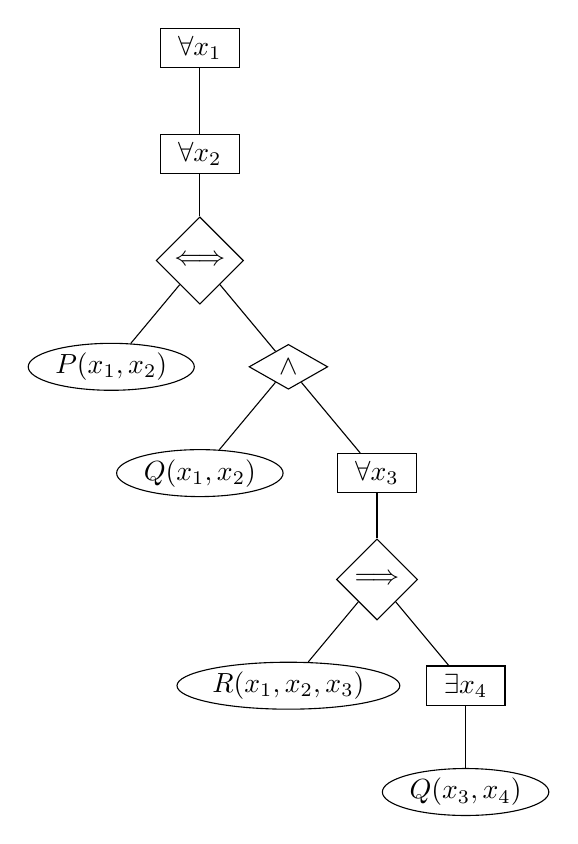
\begin{tikzpicture}[syntree, scale=0.9]
        \node[quantifier] {\(\forall x_1\)}
          child{ node [quantifier] {\(\forall x_2\)}
            child { node[connective] {\(\iff\)}
              child { node[literal] {\(P(x_1, x_2)\)} }
              child { node[connective] {\(\land\)}
                child { node[literal] {\(Q(x_1, x_2)\)} }
                child { node[quantifier] {\(\forall x_3\)}
                  child { node[connective] {\(\implies\)}
                    child { node[literal] {\(R(x_1, x_2, x_3)\)} }
                    child { node[quantifier] {\(\exists x_4\)}
                      child { node[literal] {\(Q(x_3, x_4)\)} }
                    }
                }
              }
              }
            }
          };
    \end{tikzpicture}
    \caption{Syntactic tree for last example in Equation~\ref{eq:fluted-example} without quantifiers flattening}\label{fig:fluted_syntree}
\end{figure}

\begin{figure}[H]
    \centering
    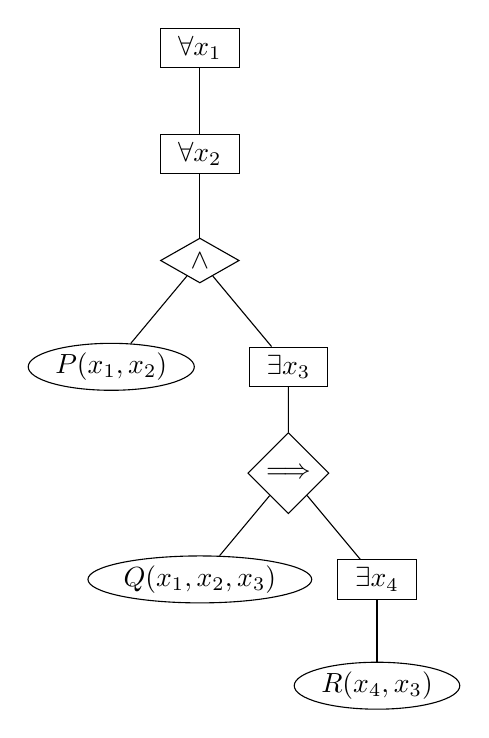
\begin{tikzpicture}[syntree,scale=0.9]
        \node[quantifier] {\(\forall x_1\)}
          child{ node [quantifier] {\(\forall x_2\)}
            child { node[connective] {\(\land\)}
              child { node[literal] {\(P(x_1, x_2)\)} }
              child { node[quantifier] {\(\exists x_3\)}
                child { node[connective] {\(\implies\)}
                  child { node[literal] {\(Q(x_1, x_2, x_3)\)} }
                  child { node[quantifier] {\(\exists x_4\)}
                    child { node[literal] {\(R(x_4, x_3)\)} }
                  }
                }
              }
            }
          };
    \end{tikzpicture}
    \caption{Syntactic tree for first example in Equation~\ref{eq:not-fluted-example} without quantifiers flattening}\label{fig:not_fluted_syntree}
\end{figure}

From the syntactic tree in Figure~\ref{fig:fluted_syntree}, it is easy to see that each atom has as arguments a suffix of the string of bound variables obtained from the traversal of the branch of the tree with the atom as leaf.
By contrast, in Figure~\ref{fig:not_fluted_syntree}, the atom \(R(x_4, x_3)\) had as argument string \(x_4 x_3\), which is not a suffix of the string of bound variables \(x_1 x_2 x_3 x_4\).
This observation leads to the fact that, in \dquote{\emph{constructing}} a fluted sentence top-down, one can only \emph{introduce} new variables at the end of the string and the variables an atom \(P\) is applied to is completely determined by the quantifiers it is in scope of and its arity, while everything remains arbitrary.

\section{Fluted Clauses}\label{sec:fluted-clauses}

In~\cite{schmidt2000resolution}, \citeauthor{schmidt2000resolution} introduces a restricted class of clauses named \bold{fluted clauses}.
These clauses are characterized by a specific structure that adheres to the constraints outlined in the previous section and such that any fluted formula, after the necessary naming, can be transformed into a fluted clause.
Before we delve into the formal definition of the fluted clauses class, we need to introduce some notation.

The notation \(\flseq{i}\) will denote a finite, possibly empty, sequence \((u_i,u_{i+1}, \ldots, u_m)\) of terms. Unless specified otherwise each non-empty sequence \(\flseq{i}\) will be assumed to end with \(u_m\).
The sequences \(\flseq{1},\flseq{2},\ldots,\flseq{m}\) are therefore linearly ordered by the converse of the proper suffix relation.
Therefore, the following notations will be used:
\begin{itemize}
  \item \(\flseq{i}[t]\) will denote the sequence \((u_i,u_{i+1}, \ldots, u_m,t)\).
  \item \(f\flseq{i}\) will denote the term \(f(u_i,u_{i+1}, \ldots, u_m)\).
  \item \(P\flseq{i}\) will denote the predicate \(P(u_i,u_{i+1}, \ldots, u_m)\).
  \item \(C\flseq{i}\) will denote a (possibly empty) clause of literals of the form \((\neg)P\flseq{i}\).
\end{itemize}

For \(f\flseq{i},P\flseq{i} \text{ and } C\flseq{i} \), \(\flseq{i}\) is called the \emph{argument sequence} of the corresponding term, predicate or clause.
If \(\flseq{i}\) is empty, then \(f\flseq{i}, P\flseq{i} \text{ and } C\flseq{i}\) respectively denote a constant, a propositional literal and a (possibly empty) propositional clause.

\begin{definition}\label{def:fluted-sequence}
Given \(m,n \in \mathbb{N} \text{ and } X_m = \{x_1,x_2,\ldots,x_m\}\) as previously defined, we will refer as to the sequence of terms \(\overline{u} = (u_1,u_2,\ldots,u_n)\) as a \emph{fluted sequence} over \(X_m\), if all the following conditions hold:
\begin{enumerate}[label= (\roman*)]
  \item \(n > m\);
  \item \(u_1=x_1,\ldots,u_m=x_m\);
  \item the number of variables occurring in \((u_{m+1},\ldots,u_n)\) is \(m\);
  \item for every \(k \in \{m+1,\ldots,n\}\), there is an \(i \in \{1,\ldots,k-1\}\) such that \\\(u_k = f(u_i,\ldots,u_{k-1})\) for some function symbol \(f\).
\end{enumerate}
The sequence \((x_1, \ldots, x_m)\) will be called the \emph{variable prefix} of \(\overline{u}\).
\end{definition}

This set of conditions serves the purpose of ensuring that the sequence of terms \(\overline{u}\) is constructed naturally extending the ordered set of variables \(X_m\) by introducing new functional terms whose argument sequences are suffixes of the \emph{fluted sequence} that precedes them.

Examples of fluted sequences are:
\begin{itemize}
  \item \((a)\), a fluted sequence over \(X_0=\emptyset\)
  \item \((x_1,x_2,x_3,f(x_1,x_2,x_3))\)
  \item \((x_1,x_2,x_3,f(x_2,x_3),g(x_1,x_2,x_3,f(x_2,x_3)))\)
  \item \((x_1,x_2,f(x_1,x_2),g(f(x_1,x_2)),h(x_2,f(x_1,x_2),g(f(x_1,x_2))))\)
\end{itemize}
while the following are not:
\begin{enumerate}[label= (\roman*)]
  \item \((x_1,x_2)\) over \(X_3\)\footnote{The sequence would have been fluted if it had been over \(X_2\) or \(X_1\).};
  \item \((x_1,x_2,f(x_3,x_4),x_3)\);
  \item \((x_1,x_2,x_3,f(x_3))\);
  \item \((x_1,x_2,x_3,f(x_3),g(x_1,x_2,x_3))\);
\end{enumerate}
because they violate respectively conditions (i), (iv), (iv) and (iv) of Definition~\ref{def:fluted-sequence}.

Moreover, these constraints ensure that the DAG representation of the fluted sequence has a unique total topological ordering providing another possible order on functional terms\footnote{Technically, the sequence ordering corresponds to the topological ordering in the \emph{transposed DAG}, with the one induced by the edges in the original DAG being its dual.}.
This can be easily shown by observing that, for every \(n\) only the vertex corresponding to \(u_n\) has in-degree zero, and therefore it must be the first vertex in any topological ordering of the DAG\@. Removing that vertex (and therefore that term) will again leave a DAG (and a fluted sequence) where only one vertex has in-degree zero (\(u_{n-1}\)), and so on until all vertices \(u_{m+1},\ldots, u_n\) are removed.

\begin{figure}[H]
\centering
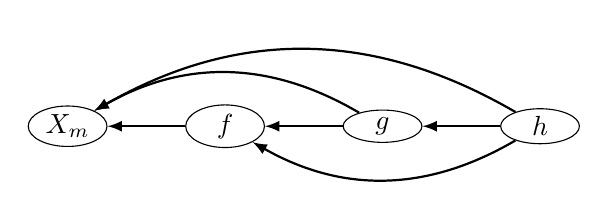
\begin{tikzpicture}[syntree]
  % Nodi
  \node[literal] (x) at (-2,0) {\(X_m\)};
  \node[literal] (f) at (0,0) {\(f\)};
  \node[literal] (g) at (2,0) {\(g\)};
  \node[literal] (h) at (4,0) {\(h\)};
  
  \draw[-latex, thick] (f) -- (x);
  \draw[-latex, thick, bend right=30] (g) to (x);
  \draw[-latex, thick] (g) -- (f);
  \draw[-latex, thick, bend right=30] (h) to (x);
  \draw[-latex, thick, bend left=30] (h) to (f);
  \draw[-latex, thick] (h) -- (g);
\end{tikzpicture}
\caption{DAG of last example of fluted sequences}\label{fig:fluted-sequence-dag}
\end{figure}
Is possible now to define the class of fluted clauses.

\begin{definition}\label{def:fluted-clauses}
  A clause \(C\) is a \emph{fluted clause} over \(X_m\) if one of the following conditions holds:
  \begin{description}
    \item[(FL0)] \(C\) is a (possibly empty) propositional clause.
    \item[(FL1)] \(C\) is not empty, the set of variables occurring in \(C\) (denoted \(\var{C}\)) is exactly \(X_m\), and for any literal \(L\) in \(C\), there is some \(i \in \{1,\ldots,m\}\) such that the argument sequence of \(L\) is
      \[(x_i, x_{i+1}, \ldots, x_m).\]
    \item[(FL2)] \(C\) is functional and not empty, \(\var{C} = X_m\), and for any literal \(L\) in \(C\), the argument sequence of \(L\) is one of
      \[(x_{i},x_{i+1}, \ldots, x_{i_m}) \text{ or }\]
      \[(u_j, u_{j+1}, \ldots, u_{n}),\]
    where \(1 \leq i \leq m\) and \((u_j, u_{j+1}, \ldots, u_{n})\) is a suffix of some fluted sequence \(\overline{u}\) over \( \{x_k, \ldots, x_m\}\) with \(k \in \{1,\ldots,m\}\).
    \(\overline{u}\) will be referred to as the \emph{fluted sequence associated} with \(L\).
    \item[(FL3)] \(C\) is not empty, \(\var{C} = X_{m+1}\), and for any literal \(L\) in \(C\), the argument sequence of \(L\) is either
      \[(x_{1},x_{2}, \ldots, x_{m}) \text{ or }\]
      \[(x_{i},x_{i+1}, \ldots, x_{m},x_{m+1}),\]
    where \(1 \leq i \leq m+1\).
  \end{description}
  A fluted clause will be called \emph{strongly fluted clause} if it is either ground or has a literal which contains all the variables of the clause.
\end{definition}
Some examples of fluted clauses are:
\begin{description}
  \item[(FL0)] \(\neg P \lor Q \lor R\)
  \item[(FL1)] \(P(x_1,x_2,x_3,x_4,x_5) \lor Q(x_1,x_2,x_3,x_4,x_5) \lor \neg R(x_4,x_5) \lor S(x_5)\)
  \item[(FL2)] \(Q(x_1,x_2) \lor R(x_2) \lor P(x_1,x_2,f(x_1,x_2))\lor R(x_2,f(x_1,x_2)) \lor S(f(x_1,x_2))\)
  \item[(FL3)] \(Q(x_1,x_2) \lor \neg P(x_1,x_2,x_3) \lor \neg R(x_2,x_3) \lor S(x_3)\)
\end{description}

Some additional notes:
\begin{enumerate*}[label= (\alph*)]
  \item The non-functional subclause of a (FL2)-clause (denoted by \(\nabla\)) satisfies (FL1), therefore (FL1)-clauses are building blocks of (FL2)-clauses.
  \item Clauses of type (FL3) are defined to be fluted clauses over \(m\) variables, even though they contain \(m+1\) variables. This is to ensure direct association of fluted formulae over \(m\) variables with fluted clauses over \(m\) variables. The previous example of (FL3)-clause is therefore over \(2\) variables.
  \item No fluted clause can simultaneously satisfy multiple fluted conditions at once.
\end{enumerate*}

Strongly fluted clauses will be the core of the resolution procedure assuring its termination.
That is because, resolving two strongly fluted clauses and selecting as eligible literal the literal containing all the variable of the clause, will produce a resolvent with a number of variables less than or equal to the number of variables of the parent clauses.
Some additional property of fluted clauses come from the following results.
The proofs follow straightforwardly and are therefore omitted for brevity. Complete demonstration for these lemmas, and for all other claims in this chapter, can be found in~\cite{hustadt2000resolution}.

\begin{lemma}\label{lem:fluted-sequence-properties}
  Let \(\overline{u}\) be a fluted sequence over \(X_m\). Then:
  \begin{enumerate}
    \item There is an element \(u_k\) of \(\overline{u}\) such that \(u_k = f(u_1,\ldots,u_{k-1})\), for some \(f\)
    \item If \(u_n\) is the last element of \(\overline{u}\), then \(\var{u_n} = X_m\)
    \item \(\overline{u}\) is uniquely determined by its last element
    \item if \(u_j, u_{j+1}, \ldots, u_n\) is a suffix of \(\overline{u}\), then \(u_1, \ldots, u_{j-1}\) is uniquely determined by \(u_j\)
  \end{enumerate}
\end{lemma}

\begin{lemma}\label{lem:var-sequence-fl2}
  Let \(L\) be any literal of a (FL2)-clause defined over \(X_m\). Then, all occurrences of variable sequences in \(L\) are suffixes of \(x_1, \ldots, x_m\).
\end{lemma}

\begin{lemma}\label{lem:strongly-fluted-clauses}
  Let \(C\) be a fluted clause over \(m\) variables. \(C\) is strongly fluted if and only if:
  \begin{enumerate*}[label= (\roman*)]
    \item \(C\) satisfies exactly one of the conditions (FL0), (FL1), (FL2), or
    \item \(C\) satisfies condition (FL3), and it contains a literal with \(m+1\) variables.
  \end{enumerate*}
\end{lemma}

Lemma~\ref{lem:strongly-fluted-clauses} is of particular relevance, because it assures that any fluted clause is indeed strongly fluted, except for some (FL3)-clauses. Those exceptions will be handled with a new inference rule named \emph{separation} that will be introduced later.

\section{From Fluted Formulae to Fluted Clauses}\label{sec:from-fluted-formulae-to-fluted-clauses}

Once defined the class of fluted clauses, a procedure to transform any fluted formula into a set of fluted clauses is needed.
This transformation is obtained by pre-pending to standard clausification defined in Section~\ref{sec:skolemization_and_normalization} a step of \emph{renaming}, as mentioned in Section~\ref{sec:auxiliary_predicate_introduction}, that guarantees the preservation of the fluted structure.
In particular, the renaming technique used is also known as \emph{structural transformation}.
To describe this \emph{renaming} step more formally it is sufficient to define a function \(t\) that maps any fluted formula \(\phi\) over \(X_m\) to a fluted formula \(t(\phi)\) over \(X_m\) that, after the standard clausification, produces a set of fluted clauses.

Let \(Pos(\phi)\) be the set of positions of a first-order formula \(\phi\). If \(\lambda\) is in \(Pos(\phi)\), then \(\phi|_\lambda\) denotes the subformula of \(\phi\) at position \(\lambda\) and, extending the previously introduced notation for substitution, \(\phi[\psi\mapsto\lambda]\) is the result of replacing \(\phi|_\lambda\)  at position \(\lambda\) with \(\psi\).

Looking at formulae from the prospective of their syntactic tree, \(Pos(\phi)\) can be seen as the ordered set of all nodes in the tree visited in a pre-order traversal, \(\phi|_\lambda\) is the subtree rooted at node \(\lambda\), and \(\phi[\psi\mapsto\lambda]\) is tree obtained by replacing the subtree rooted at node \(\lambda\) with the tree of \(\psi\).
Structural transformations associates with each element \(\lambda \in \Lambda \subseteq Pos(\phi)\) a fresh predicate symbol \(Q_\lambda\) and a literal \(Q_\lambda(x_1,\ldots,x_n)\), where \(x_1,\ldots,x_n\) are the free variables of \(\phi|_\lambda\), such that any two symbols \(Q_\lambda \text{ and } Q_{\lambda'}\) are equal only if \(\phi|_\lambda\) and \(\phi|_{\lambda'}\) are equivalent formulae.

Given 
  \[\fldef{\lambda}[+]{\phi} = \forall x_1, \ldots, x_n(Q_\lambda(x_1,\ldots,x_n)\implies \phi|_\lambda) \text{ and}\]
  \[\fldef{\lambda}[-]{\phi} = \forall x_1, \ldots, x_n(\phi|_\lambda \implies Q_\lambda(x_1,\ldots,x_n)).\]

we define the \emph{definition} of \(Q_\lambda\) as the formula
\begin{equation}
  \fldef{\lambda}{\phi} = \begin{cases}
                        \fldef{\lambda}[+]{\phi} & \text{if } \phi|_\lambda \text{has positive polarity}\\
                        \fldef{\lambda}[-]{\phi} & \text{if } \phi|_\lambda \text{has negative polarity}\\
                        \fldef{\lambda}[+]{\phi} \land \fldef{\lambda}[-]{\phi} & \text{otherwise}
                      \end{cases}
\end{equation}
The corresponding clauses are called \emph{definitional clauses}.

Is possible to inductively extends \emph{definition} to the whole set of positions \(\Lambda\) (\(Def_\Lambda(\phi)\)) as follows:
\begin{equation}
  \begin{aligned}
    \fldef{\emptyset}{\phi} &= \phi\\
    \fldef{\Lambda\cup\{\lambda\}}{\phi} &= \fldef{\Lambda}{\phi[Q_\lambda(x_1,\ldots,x_n)\mapsto\lambda]} \land \fldef{\lambda}{\phi}
  \end{aligned}
\end{equation}
\indent where \(\lambda\) is maximal in \(\Lambda\cup\{\lambda\}\) with respect to the prefix ordering on positions.
For any first-order formula \(\phi\), \(\fldef{\Lambda}{\phi}\) will denote the \emph{definitional form} obtained by introducing new names for subformulae at positions in \(\Lambda\).
This transformation can be seen as substituting each node of the syntactic tree in \(\Lambda\) with a fresh literal \(Q_\lambda(x_1,\ldots,x_n)\) in post-order, adding the definition of \(Q_\lambda\) as a child of a new root node for the \(\land\) connective.

\begin{figure}[H]
  \centering
  \begin{minipage}[t]{.3\textwidth}
    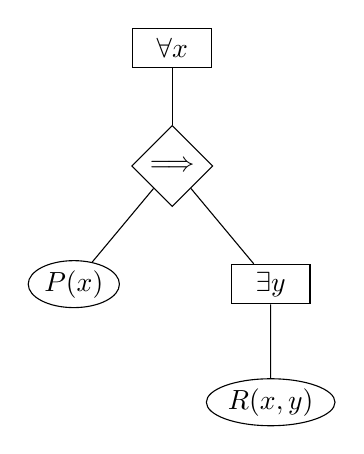
\begin{tikzpicture}[syntree]
      \node[quantifier] {\(\forall x\)}
            child { node[connective] {\(\implies\)}
              child { node[literal] {\(P(x)\)} }
              child { node[quantifier] {\(\exists y\)}
                  child { node[literal] {\(R(x, y)\)} }
              }
            };
    \end{tikzpicture}
  \end{minipage}
  \begin{minipage}[t]{.3\textwidth}
    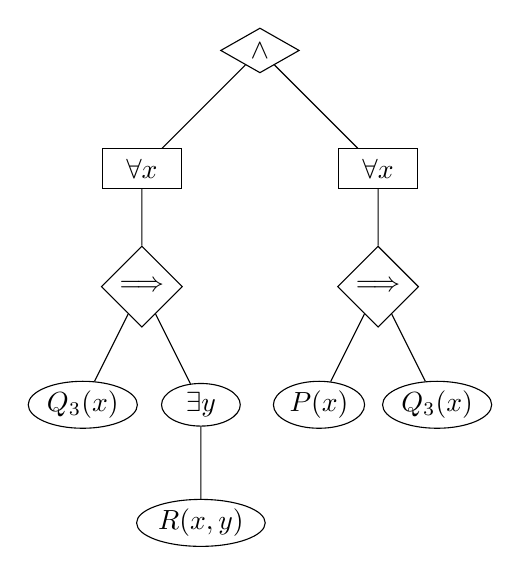
\begin{tikzpicture}[syntree,
                        level 1/.style={sibling distance=3cm},
                        level 2/.style={sibling distance=2cm},
                        level 3/.style={sibling distance=1.5cm}
                        ]
      \node[connective] {\(\land\)}
            child {node[quantifier] {\(\forall x\)}
              child { node[connective] {\(\implies\)}
                child { node[literal] {\(Q_3(x)\)} }
                child { node[literal] {\(\exists y\)}
                  child { node[literal] {\(R(x, y)\)} }
                }
              }
            }
            child{node[quantifier] {\(\forall x\)}
              child { node[connective] {\(\implies\)}
                child { node[literal] {\(P(x)\)} }
                child { node[literal] {\(Q_3(x)\)} }
              }
            };
    \end{tikzpicture}
  \end{minipage}
  \caption{Structural transformation of a formula into its definitional form with \(\Lambda = \{3\}\).}\label{fig:definitional-form}
\end{figure}

Usually \(\Lambda\) is the subset of all positions of subformulae which are non-atomic or non-literal.
For the problem of decidability is important that this transformation preserves satisfiability. Indeed, the following theorem holds:

\begin{theorem}\label{thm:definitional-sat-preservation}
  Let \(\phi\) be a first-order formula. For any \(\Lambda \subseteq Pos(\phi)\),
  \begin{enumerate}
    \item \(\phi\) is satisfiable if and only if \(\fldef{\Lambda}{\phi}\) is satisfiable;
    \item \(\fldef{\Lambda}{\phi}\) can be computed in polynomial time.
  \end{enumerate}
\end{theorem} 
It is therefore possible to show that any fluted formula \(\phi\), introducing new literals for each non-literal subformula position, can be transformed into a set of strongly fluted clauses.

\begin{lemma}
  Let \(\phi\) be any fluted formula. If \(\Lambda\) contains all non-literal subformulae positions of \(\phi\) then the clausification of \(\fldef{\Lambda}{\phi}\) is a set of strongly fluted clauses (provided the newly introduced literals have the form \((\neg)Q_\lambda(\overline{x}_i)\)).
\end{lemma}
To instead obtain a set of fluted clauses (not necessarily strongly fluted) it is required to introduce new symbols only for the quantified subformulae\footnote{
  Strictly speaking, in~\cite{hustadt2000resolution} is mentioned, that only requires the introduction of new symbols for positive occurrences of universally quantified subformulae, negative occurrences of existentially quantified subformulae and all quantified subformulae with zero polarity, but then another form of Skolemization needs to be used.
}.

\begin{lemma}\label{lem:fluted-def-constraints}
  Let \(\phi\) be any fluted formula over \(X_m\). If \(\Lambda\) contains at least the positions of any subformulae \(\exists x_{i+1}\psi, \forall x_{i+1}\psi\), then the clausification of \(\fldef{\Lambda}{\phi}\) is a set of fluted clauses (again, provided the newly introduced literals have the form \((\neg)Q_\lambda(\overline{x}_i)\)).
\end{lemma}

The loss of the strong property of the generated clauses is due to \(\fldef{\lambda}[-]{\phi}\) of existentially quantified subformulae (and to \(\fldef{\lambda}[+]{\phi}\) of universally quantified subformulae by duality).
This is easy to show considering the subformula at position \(\lambda\):
  \[
    \exists x_3 (P(x_1,x_2,x_3) \lor R(x_2,x_3))
  \]
that leads to the negative definition
  \[
    \fldef{\lambda}[-]{\phi} = \forall x_1,x_2(\exists x_3 (P(x_1,x_2,x_3) \lor R(x_2,x_3)) \implies Q_\lambda(x_1,x_2))
  \]
whose clausification produces the (FL3)-clauses
  \[
    Q_\lambda(x_1,x_2) \lor \neg P(x_1,x_2,x_3)
  \]
  \[
    Q_\lambda(x_1,x_2) \lor \neg R(x_2,x_3)
  \]
of which the latter does not contain a literal which contains all the variables of the clause, and is thus only fluted, not strongly fluted.

Having potentially non-strongly fluted clauses in this phase is not a problem because, as we will see later, resolution of strongly fluted clauses can produce a non-strongly fluted clause, making a procedure to obtain equivalent strongly fluted clauses from non-strongly fluted ones necessary anyway.
This procedure is the new inference rule named \bold{separation}.
\section{Separation}\label{sec:separation}
As briefly mentioned in the previous section, the motivation for introducing the \emph{separation} inference rule is that the class of fluted clauses is not closed under resolution.
In particular, resolvents of non-strongly fluted (FL3)-clauses are not always fluted and can cause (potentially) unbound variable chaining across literals.
This can be shown considering the resolution between
  \[
    P_1(x_1,x_2) \lor Q_1(x_2,x_3) \lor R(x_2,x_3) \text{ and }
  \]
  \[
  \neg R(x_1,x_2) \lor P_2(x_1,x_2) \lor Q_2(x_2,x_3)
  \]
which produces the resolvent
  \[
    P_1(x_1,x_2) \lor Q_1(x_2,x_3) \lor P_2(x_2,x_3) \lor Q_2(x_3,x_4)
  \]
that is not fluted and contains more variables than the original clauses.
The class of strongly fluted clauses is also not closed under resolution but, inferences with two strongly fluted clauses always produce fluted clauses. Having a procedure to make non-strongly fluted clauses into strongly ones would close the circle, making the set of strongly fluted clauses closed under the application of resolution followed by such procedure.

Consider the strongly fluted clauses
  \[
    P(x_1,x_2) \lor R(x_1,x_2,x_3) \text{ and }
  \]
  \[
  \neg R(x_1,x_2,x_3) \lor P(x_2,x_3)
  \]
whose resolvent is
  \[
    C = P(x_1,x_2) \lor P(x_2,x_3)
  \]

\(C\) satisfies (FL3) but it is not strongly fluted, as none of its literals contains all the variables of the clause.
A consequence of this, is that the literals are incomparable under an admissible ordering (in particular, a liftable ordering), because the literals have a common instance, for example
  \[
    C\{x_1 \mapsto a, x_2 \mapsto a, x_3 \mapsto a\} = P(a,a) \lor P(a,a)
  \]
The problem is caused by the variable \(x_1 \text{ and } x_3\). Because they do not occur together in any literal, \(C\) can be separated and replaced by the following two clauses, where \(Q\) is a new predicate symbol.
  \[
    Q(x_2) \lor P(x_1,x_2)
  \]
  \[
    \neg Q(x_2) \lor P(x_2,x_3)
  \]
These two clauses are indeed strongly fluted, the first satisfying (FL1) and the second (FL3) but being strongly fluted.
This process of separating non-strongly fluted clauses into strongly fluted ones can be formalized in the \bold{separation} inference rule, that can be used outside the context of fluted logic as well.

\begin{definition}
  Let \(C\) be an arbitrary clause. \(C\) is \bold{separable} if it can be partitioned into two non-empty subclauses \(D_1\) and \(D_2\) such that \(\var{D_1} \not\subseteq \var{D_2} \text{ and } \var{D_2} \not\subseteq \var{D_1}\)
\end{definition}
\noindent For example the clause shown before is separable, while the clause \(P(x_1,x_2) \lor Q(x_2,x_3) \lor R(x_1,x_3)\) is not.
\begin{theorem}\label{thm:separation}
  Let \(C \lor D\) be a separable clause such that \(\var{C} \cap \var{D} = \{x_1,\ldots,x_n\}\) for \(n \in \mathbb{N}\).
  Let \(Q\) be a fresh predicate symbol with arity \(n\).
  Then a set of clauses \(N \cup \{C\lor D\}\) is satisfiable if and only if the set of clauses \(N \cup \{\neg Q(x_1,\ldots, x_n) \lor C, Q(x_1,\ldots, x_n) \lor D\}\) is satisfiable.
\end{theorem}
On the basis of this theorem we can define the following replacement rule:

\begin{equation}\label{eq:separation-rule}
  \bold{Separation:} \quad \infer{N \cup \{\neg Q(x_1,\ldots, x_n) \lor C, Q(x_1,\ldots, x_n) \lor D\}}{N \cup \{C \lor D\}}
\end{equation}
\indent provided 
\begin{enumerate*}[label = (\roman*)]
  \item \(C \lor D\) is separable,
  \item \(\var{C} \cap \var{D} = \{x_1,\ldots,x_n\}\) for \(n \in \mathbb{N}\),
  \item \(Q\) is \indent a fresh predicate symbol with arity \(n\).
\end{enumerate*}

\noindent From the definition of separable clauses, also follows that
\begin{lemma}\label{lem:separation-replacement}
  The replacements of a separable clause \(C\) each contain less variable than \(C\)
\end{lemma}
Moreover, it is possible to prove the following.

\begin{theorem}
  Let \(R^{sep}\) denote the extension of \(R\) defined as in Section~\ref{sec:resolution-factoring} with the separation inference rule and let \(N\) be a set of clauses.
  Then \(N\) is unsatisfiable if and only if the saturation of \(N\) under \(R^{sep}\) contains the empty clause.
\end{theorem}
More generally, this theorem holds also if \(R^{sep}\) is based on ordered resolution

By Lemma~\ref{lem:strongly-fluted-clauses}, separable fluted clauses have the form
\begin{equation}\label{eq:separable-fluted-clauses}
  \mathcal{L}(\overline{x}_1)\lor \mathcal{L}\flseq[x]{i}[x_{m+1}] \lor \ldots \lor \mathcal{L}(x_m, x_{m+1}) \lor \mathcal{L}(x_{m+1})
\end{equation}
where \(\mathcal{L}(\cdot)\) denotes a (possibly empty) disjunction of literals with non-empty argument sequence \((\cdot)\), \(\mathcal{L}\flseq[x]{1}\) is not empty and \(i\) is the smallest integer in \(\{2,\ldots, m\}\) such that \(\mathcal{L}\flseq[x]{i}[x_{m+1}]\) is not empty.

The separation of clauses in this form, will produce clauses with the form
\[
  \neg Q(\overline{x}_i) \lor \mathcal{L}(\overline{x}_1) \text{ and }
\]
\[
  Q(\overline{x}_i) \lor \mathcal{L}(\overline{x}_i,x_{m+1}) \lor \ldots \lor \mathcal{L}(x_m, x_{m+1}) \lor \mathcal{L}(x_{m+1})
\]
which are obviously strongly fluted, thanks to literals in \(\mathcal{L}(\overline{x}_1)\) and in \(\mathcal{L}(\overline{x}_i,x_{m+1})\).

From this consideration, follows that:
\begin{lemma}\label{lem:separation-fluted}
  The separation of a separable fluted clause is a set of strongly fluted clauses
\end{lemma}
\begin{lemma}
  For fluted clauses a separation inference step can be performed in linear time
\end{lemma}


\section{Fluted Resolution}\label{sec:fluted-resolution}

In the end, we can formally define an ordered resolution based inference system \(R^{sep}\) whose application is a decision procedure for fluted logic.
The ordering \(\succ\) of \(R^{sep}\) is required to be any admissible ordering compatible with the following complexity measure.

\begin{definition}
  Let \(\succ_s\) denote the proper super-term ordering. Define the complexity measure of any literal \(L\) by \(c_L = (ar(L),max(L),sign(L))\), where \(ar(L)\) is the arity of \(L\), \(max(L)\) is a \(\succ_s\)-maximal term occurring in \(L\) and \(sign(L)\) is \(1\) if \(L\) is negative and \(0\) if \(L\) is positive. % chktex 35
  The ordering on the complexity measures is given by the lexicographic combination of \(>,\succ_s \text{ and } >\), where \(>\) is the usual ordering on natural numbers.
\end{definition}
Having the ordering \(\succ\) in place, we can now define the inference system \(R^{sep}\) more formally.

\begin{definition}
  Let \(R^{sep}\) be any inference system in which
  \begin{enumerate*}[label = (\roman*)]
    \item derivations are generated by removing redundant literals, separating separable clauses and deducing new clauses with the inferences in \(R\) in this order
    \item the ordering is based on \(\succ\), defined above.
  \end{enumerate*}
\end{definition}
It can be shown that the class of fluted clauses is closed under the inference system \(R^{sep}\) by the following lemmas.

\begin{lemma}\label{lem:factor-strongly-fluted}
  A factor of a strongly fluted clause \(C\) is again a strongly fluted clause of the same type.
\end{lemma}
In fact, any (unordered) factor of a strongly fluted clause \(C\) is again a strongly fluted clause of the same type.

\begin{lemma}
  Let \(C = C' \lor A_1\) and \(D = \neg A_2 \lor D'\) be (FL2)-clauses.
  Suppose \(A_1\) and \(A_2\) are eligible literals in \(C\) and \(D\) respectively, and that \(\sigma\) is the MGU of \(A_1\) and \(A_2\).
  Then:
  \begin{enumerate}
    \item \(C\sigma\), \(D\sigma\) and \(C\sigma \lor D\sigma\) are (FL2)-clauses.
    \item For any functional literal \(L\sigma\) in \(C\sigma \lor D\sigma\), the fluted sequence associated with \(L\sigma\) is the \(\sigma\)-instance of a fluted sequence \(\overline{v}\) associated with some literal \(L'\) in \(C \lor D\).
  \end{enumerate}
\end{lemma}
This lemma is the most important technical result of~\cite{hustadt2000resolution} because with it, we can easily show that the resolution of strongly fluted clauses involving (FL2)-clauses always produce strongly fluted clauses.
\begin{lemma}\label{lem:union-strongly-fluted}
  Let \(C = C' \lor A_1\) and \(D = \neg A_2 \lor D'\) be strongly fluted clauses. Suppose \(A_1\) and \(A_2\) are eligible literals in \(C\) and \(D\) respectively, and that \(\sigma\) is the MGU of \(A_1\) and \(A_2\).
  Then \(C\sigma \lor D\sigma\) is a strongly fluted clause.
\end{lemma}
\begin{lemma}\label{lem:removal-fluted}
  Removing any subclause from a fluted clause produces a fluted clause.
\end{lemma}
The combination of Lemmas~\ref{lem:union-strongly-fluted} and~\ref{lem:removal-fluted} leads to the closure of strongly fluted clauses under ordered resolution in the broader sense of closure mentioned above.

\begin{lemma}\label{lem:resolution-fluted}
  The resolvent of any two strongly fluted clauses is a strongly fluted clause, or, it is only a fluted clause, if one of the premises is a (FL3)-clause
\end{lemma}
Moreover, it can be shown that:

\begin{lemma}\label{lem:size-fluted}
  Let \(C,D\) and \(\sigma\) defined as in Lemma~\ref{lem:union-strongly-fluted}. Then,
  \[ |\var{C\sigma \lor D\sigma} \leq \max\{ |\var{C\sigma}|,|\var{D\sigma}|\}\]
\end{lemma}
Finally, by Lemmas~\ref{lem:separation-fluted},~\ref{lem:factor-strongly-fluted} and~\ref{lem:resolution-fluted}, we can conclude that:
\begin{lemma}
  Any separated factor or resolvent of strongly fluted clauses is strongly fluted.
\end{lemma}
In the end, remains only to show that the application of \(R^{sep}\) constitutes a decision procedure for fluted logic, and so does terminate on each finite input set of clauses.

For doing this it is usually sufficient~\cite{joyner1976resolution} to show that:
\begin{enumerate}[label= (\roman*)]
  \item\label{item:bounded-variables} the number of variables in any derivable clause is finitely bounded;
  \item\label{item:bounded-depth} there is a bound on the depth of terms occurring in derived clauses;
  
  Because separation introduces new predicate names during the derivation, in our case we also need to show that:
  \item\label{item:bounded-separation} there is a bound on the number of applications of the separation rule.
\end{enumerate}

From Lemmas~\ref{lem:separation-replacement} and~\ref{lem:size-fluted}, follows immediately~\ref{item:bounded-variables} by:
\begin{lemma}\label{lem:bounded-variables}
  All clauses occurring in an (\(R^{sep}\))-derivation from \(N\) contain at most \(m+1\) variables, where \(m\) is the maximal arity of any predicate symbol in \(N\)
\end{lemma}
The definition of fluted clauses places no restriction on the level of nesting of functional terms, but:
\begin{lemma}\label{lem:bounded-depth}
  A bound on the maximal term depth of clauses derived by \(R^{sep}\) from \(N\) is \(m\), where \(m\) is the maximal arity of any predicate symbol in \(N\)
\end{lemma}
This lemma can be shown by observing that, as a consequence of Lemma~\ref{lem:strongly-fluted-clauses}, the maximal length of any fluted sequences associated with literals in inferred clauses does not increase and that the maximal term depth of any term is the length of the fluted sequence associated with it.
It follows that the maximal term depth for any derived clause is the maximal length of any fluted sequence of a literal in \(N\) that, is obviously \(m\), the maximal arity of any predicate symbol in \(N\).

Finally, remains to show~\ref{item:bounded-separation}.
\begin{lemma}\label{lem:bounded-separation}
  The number of applications of the separation rule in any (\(R^{sep}\))-derivation from \(N\) is bounded.
\end{lemma}

The idea of the proof is that the newly introduced literals is never eligible in the new clauses because its arity is always less than some literal in the clause.
Therefore, the two replacement of a separated clause cannot be resolved together recreating the original clause. The literals become eligible only when all other \dquoteit{bigger} literals are removed, leading to a non-increase of arity.

The theoretical discussion of the fluted fragment can therefore be said to be concluded with the enunciation of the last final theorem deriving directly from the previous lemmas.

\begin{theorem}
  Let \(\phi\) be any fluted formula and \(N\) be the clausification of \(\fldef{\Lambda}{\phi}\) satisfying the restrictions of Lemma~\ref{lem:fluted-def-constraints}.
  Then:
  \begin{itemize}
    \item Any \(R^{sep}\)-derivation from \(N\) terminates.
    \item \(\phi\) is unsatisfiable if and only if the \(R^{sep}\)-saturation of \(N\) contains the empty clause.
  \end{itemize}
\end{theorem}

\begin{proof}
  Termination is a consequence of Lemmas~\ref{lem:bounded-variables},~\ref{lem:bounded-depth} and~\ref{lem:bounded-separation}, while soundness and completeness follows from~\cite{robinson1965} alongside Theorems~\ref{thm:definitional-sat-preservation} and~\ref{thm:separation}, in conjunction with Lemma~\ref{lem:bounded-separation}
  \qed{}
\end{proof}





    \chapter{Vampire Theorem Prover}\label{chap:vampire-theorem-prover}
Vampire~\cite{AVATAR,kovacs2013vampire,riazanov2002design} is a state-of-the-art first-order theorem prover written in C++ that employs a sophisticated array of techniques to automate reasoning tasks, including resolution-based methods, superposition calculus, and various preprocessing strategies.
It is widely used in both academic research and industrial applications for its efficiency and effectiveness in solving complex logical problems across diverse domains.
Its open-source nature and carefully designed modular architecture allow for easy integration of new techniques and algorithms, making it a flexible and extensible platform for researchers and practitioners in automated reasoning.

The system's development began in 1998 as a research project by \citeauthor{riazanov2002design} at the University of Manchester, and it is currently maintained by a broader team in the Computer Science department.
Over more than two decades of active development, Vampire has evolved into one of the most sophisticated theorem provers available, incorporating numerous theoretical advances from the automated reasoning community and practical optimizations derived from extensive empirical evaluation.
This long development history has resulted in a mature system that balances theoretical soundness with practical performance considerations.

Vampire's most defining quality is its exceptional efficiency, which has been the primary focus of its development and a key factor in establishing its prominence within the automated theorem proving community.
This efficiency is consistently demonstrated through its outstanding performance in the annual CADE ATP System Competition (CASC), the premier international competition for automated theorem provers.
Vampire has maintained a position among the top-performing systems for many years, winning in at least one category annually and achieving a particularly impressive milestone in 2025 when Vampire 5.0 secured victories in all competition categories.
These consistent competitive successes reflect not only the system's computational efficiency but also the effectiveness of its proof search strategies and heuristic selection mechanisms.

However, this relentless focus on efficiency has resulted in significant trade-offs regarding code readability and maintainability.
While the high-level architecture and component design are well-documented in various academic papers, the actual implementation is often complex and lacks comprehensive documentation.
This complexity makes it challenging for new contributors to understand and work with the codebase, frequently requiring them to \dquoteit{reverse engineer} existing functionality to understand the intricate details of specific algorithms and their implementations.
The situation is further complicated by recent development efforts that, while attempting to improve code organization, have removed, replaced, or restructured several components, making extensions written for previous versions incompatible with newer releases.
This creates additional challenges for researchers who have invested effort in developing custom modifications to the system.

This chapter discusses, from a high-level perspective, the components of Vampire that are necessary for implementing the decision procedure for the fluted fragment and that are involved in the experimental analysis presented in this thesis.
It should be noted that both this description and the development work are based on Vampire version 4.9, which is the latest version available at the time of writing.

\section{Components Overview}\label{sec:components-overview}

\begin{figure}[htbp]
  \centering
  \includegraphics[width=0.8\textwidth]{Vampire-package-diagram.pdf}
  \caption{Vampire theorem prover modular architecture overview.}\label{fig:vampire-architecture}
\end{figure}

Vampire's architecture is organized around a modular design that divides computational responsibilities across distinct modules, each handling specific aspects of the theorem proving process.

The \code{Kernel} module serves as the central component containing the system's fundamental data structures and control mechanisms.
This module houses representations for \bold{terms}, \bold{clauses}, and \bold{formulas}, which form the basic building blocks of first-order logic manipulation within Vampire.
The Kernel also contains the \code{Main Loop} of the program, which coordinates the overall execution flow and manages interactions between the various modules.

Several modules address specific computational tasks within the theorem proving process.
The \code{Parse} module handles the parsing of input problems expressed in various standard formats.
The \code{Saturation} module implements the saturation algorithms that drive the theorem proving process, systematically exploring logical consequences through controlled inference generation and clause management.
The \code{Inferences} module provides implementations of the inference rules employed during saturation, encapsulating the logical transformations that generate new clauses from existing ones.

The system includes several utility modules that provide supporting functionality.
The \code{Lib} module contains fundamental data structures used throughout the system, along with utility functions for manipulating these structures.
These components are designed to handle the specific access patterns and performance requirements typical of theorem proving applications.

The \code{Indexing} module provides data structures and algorithms for efficient storage, retrieval, and matching of terms during the reasoning process.
This module enables unification operations and term matching, which are required for the application of inference rules.
The performance characteristics of these indexing mechanisms directly affect the overall speed of the theorem prover.

User interaction and system configuration are managed by the \code{Shell} module, which handles command-line argument processing, configuration file management, and the various options that control Vampire's behaviour during execution.
This module translates user specifications and problem files into the internal representations required by the core modules.
It also contains preprocessing functionality to prepare the input for the theorem proving process.

Finally, the \code{Debug} module provides infrastructure for performance analysis and system monitoring.
It contains classes and macros for time measurements, statistics collection, and debugging support that enable performance analysis and system optimization.

\section{Problems Representation}\label{sec:problems-representation}

Vampire represents logical problems using a combination of data structures that encapsulate the various components of first-order logic.

\subsection{Terms and Literals}\label{subsec:terms-and-literals}

As discussed earlier, terms and literals are the basic building blocks of first-order logic expressions, and they therefore need to be represented in the most efficient way possible.

In Vampire, terms are represented by the \code{TermList} class, implemented as a \code{union} that can encapsulate different types of terms, including variables, constants, and function applications.
If \code{TermList} represents a variable, it stores an \code{unsigned integer} identifier that uniquely identifies it, while for complex terms it stores a pointer to a \code{Term} object, that actually represents the term.
A \code{TermList} can also store a 64 bit \code{BitField}, named \code{info}, which is used to store term-specific information.
The \code{Term} class contains the function symbol represented by a globally unique \code{unsigned integer} defined by the \code{Signature} class, which contains information about the function's arity, name and index.
Moreover, the \code{Term} contains a \code{TermList Array} of size equal to \(n+1\) where \(n\) is the function's arity.
This \code{Array} stores arguments term from right to left, reserving index \(0\) for storing term's information via the \code{info} field.
In addition, literals are represented by the \code{Literal} class, which is subclass of \code{Term}, unifying the representation of literals and functions, whose symbols are in fact both represented in \code{Signature} without any distinction.

\begin{figure}[htbp]
  \centering
  \includegraphics[width=0.8\textwidth]{Terms-and-literals.pdf}
  \caption{Terms and literals representation in Vampire.}\label{fig:terms-representation}
\end{figure}

Terms, and therefore literals, are represented by their DAG representation, in structure called \emph{Perfectly Shared} because their key principle is that everything that can be shared is shared.
In Figure~\ref{fig:dag_representation}, we illustrate the concrete representations of literals \(P(x_2,g(x_2),f(x_1,x_2,g(x_2)))\) and \(Q(x_1,x_2,g(x_1))\).

\begin{figure}[htbp]
  \centering
  \includegraphics[width=0.9\textwidth]{Perfectly-shared-literals.pdf}
  \caption{DAG representation of literals \(P(x_2,g(x_2),f(x_1,x_2,g(x_2)))\) and \(Q(x_1,x_2,g(x_1))\).}\label{fig:dag_representation}

\end{figure}

\subsection{Clauses, Formulae and Units}\label{subsec:clauses-formulae-units}


Vampire represents input problems through a hierarchical structure that provides a unified framework for handling various types of logical statements.
At the top level, each input problem is encapsulated within a \code{Problem} class instance, which serves as the primary container for all logical content and associated metadata.

The core of this representation lies in the \code{UnitList} component, which is maintained as a member of the \code{Problem} class.
This \code{UnitList} contains a collection of \code{Unit} objects, each representing an individual logical statement from the input problem.
These \code{Unit} objects collectively represent the axioms, assumptions, and assertions that define the logical context of the problem being solved.

From a logical perspective, the \code{UnitList} can be interpreted as a large conjunction \(A_1 \land A_2 \land \ldots \land A_n\), where each \(A_i\) corresponds to an individual \code{Unit} in the list.
This conjunctive interpretation reflects the assumption that all statements in the problem are simultaneously true, forming the foundation upon which reasoning proceeds.

When the input problem includes a conjecture \(C\) that needs to be proven, Vampire employs the classical proof by refutation strategy.
Rather than attempting to derive the conjecture directly from the given axioms, the system negates the conjecture to obtain \(\neg C\) and adds this negated formula to the existing \code{Unit} list.
The resulting logical system becomes \(A_1 \land A_2 \land \ldots \land A_n \land \neg C\), and Vampire then searches for unsatisfiability in this augmented formula set.
If unsatisfiability is detected, this constitutes a proof that the original conjecture \(C\) follows logically from the given axioms.

The individual \code{Unit} objects within the \code{UnitList} can take one of two distinct forms.
A \code{Unit} may be represented as a \code{Clause} object, which directly contains a clause in conjunctive normal form, represented as a list of \code{Literal} objects.

\begin{figure}[H]
  \centering
  \includegraphics[width=0.6\textwidth]{Unit.pdf}
  \caption{Clause representation in Vampire.}\label{fig:clause-representation}
\end{figure}



Alternatively, it may be represented as a \code{FormulaUnit}, which contains a pointer to a separate \code{Formula} object that can represent more complex logical structures that have not yet been converted to clausal form.

\code{Formula} objects resemble closely the syntactic tree representation of logical formulas showed in Figure~\ref{fig:syntactic_tree}.\ \code{Formula} class is in fact \emph{abstract}, specialized into several subclasses representing different syntactic constructs.
All of these subclasses, represent a subtree with the specific syntactic structure of the formula they represent as root.
These subclasses are:

\begin{description}
  \item[AtomicFormula]  Represents a basic atomic formula, composed by just one literal represented as a \code{Literal} object and is the only subclass not having continuation, representing a single-leaf tree.
  \item[QuantifiedFormula]  Represents a formula whose syntactic tree has a quantifier as root.
                            For compactness, if multiple consecutive quantifiers of the same type are present, they are represented with a single \code{QuantifiedFormula} object.
                            This class contains in fact a \code{VList}, a list of variables, storing the variables that are quantified by the sequence of quantifiers represented by the object.
                            It contains only one continuation \code{arg}, which is the subtree representing the formula being quantified.
  \item[NegatedFormula] Represents a formula whose syntactic tree has a negation as root.
                        As for the \code{QuantifiedFormula}, it contains a single continuation \code{f}, which is the subtree representing the formula being negated.
  \item[BinaryFormula]  Represents a formula whose syntactic tree has an implication, a biconditional or an exclusive disjunction\footnote{
                        Exclusive disjunction was not previously discussed because is equivalent to negated biconditional and, therefore, redundant for the purpose of previous sections} as root.
                        They clearly contain two continuations \code{lhs} and \code{rhs}, representing the left-hand side and right-hand side subformulae, respectively.
  \item[JunctionFormula]  Represents a formula whose syntactic tree has a conjunction or disjunction as root.
                          This class exploits the associativity of these connectives to compact multiple consecutive junctions into a single object.
                          This class contains in fact as continuation a \code{FormulaList}, a list of subformulae that are conjoined or disjoined together.
\end{description}

\begin{figure}[htbp]
  \centering
  \includegraphics[width=0.8\textwidth]{Formula.pdf}
  \caption{Formula representation in Vampire.}\label{fig:formula-representation}
\end{figure}

The separation of binary operators in two distinct classes, those being \code{BinaryFormula} and \code{JunctionFormula}, with different structure and behaviour, allows Vampire to handle preprocessing steps better.
Indeed, these two classes represent the binary connective normalized and removed in NNF and CNF transformation, respectively.

This dual representation scheme allows Vampire to handle both preprocessed clausal input and more complex formula structures within the same unified framework
The \code{Clause} representation is typically used for statements that have already undergone preprocessing transformations such as skolemization and conversion to conjunctive normal form.
The \code{FormulaUnit} representation, on the other hand, provides flexibility for handling complex logical statements that may require additional processing steps before being suitable for resolution-based reasoning.

\section{Preprocessing}\label{sec:preprocessing}

The preprocessing phase in Vampire is crucial for transforming input problems into a more manageable form
As discussed in Chapter~\ref{chap:first-order-logic} and~\ref{chap:inference-systems}, resolution based inference systems require input problems to be in clausal form, which is not always the case for problems expressed in first-order logic.
Therefore, a clausification procedure resembling the one summarized in Figure~\ref{fig:nnf-to-cnf-pipeline} needs to be applied to convert the input problem into a manageable form for saturation algorithms.

Alongside the usual clausification steps, Vampire applies several additional preprocessing techniques to optimize the problem representation and enhance the efficiency of the subsequent reasoning process.
Preprocessing steps do not exceed \(O(n\log{n})\) time complexity and non-essential ones can be activated or deactivated at will by the command line or via flags.
Below are the main steps of vampire preprocessing\footnote{The steps in \emph{italic} are optional and can be toggled.}:

\begin{description}
  \item[Rectification]  ensures that formulae are indeed sentences.
                        If it is not the case, free variables are quantified.
                        Moreover, it checks that no variable is quantified more than once.
  \item[True and False Simplification] simplifies formulae by eliminating trivial \(\top\) and \(\bot\).
  \item[Flattening] aggregates consecutive junctions or quantifications of the same type into a single object.
                    For example, the formula \((A \land B) \land C\) is transformed into \(A \land B \land C \).
  \item[\emph{Unused definition and pure predicate removal}]  removes or simplifies formulae of the form \(\forall x_1,\ldots,x_n P(x_1, \ldots,x_n) \iff \phi\).
                                                              If \(P\) does not occur anywhere else in the problem, the formula can be removed.
                                                              If it appears only positively (negatively), \(\iff\) can be replaced with \(\implies\) (\(\impliedby\)).
  \item[ENNF] transforms the formula into \emph{Extended Negated Normal Form}, or sometimes called \emph{Equivalence Negated Normal Form}, a variant of NNF which allows biconditionals.
  \item[\emph{Naming}] applies a naming technique to avoid search-space explosion by introducing new constants for complex subformulae as briefly mentioned in Section~\ref{sec:auxiliary_predicate_introduction}.
  \item[NNF] transforms the formula into \emph{Negated Normal Form} removing all binary connectives but junctions and pushing negations to atomic formulae as described in Subsection~\ref{subsec:negated_normal_form}.
  \item[Skolemization] removes existential quantifiers by introducing Skolem functions, as described in Subsection~\ref{subsec:skolemization}.
  \item[Clausification] complete the preprocessing procedure by dropping universal quantifiers and transforming the formula into \emph{Clausal Normal Form}, as described in Subsection~\ref{subsec:clausal_normal_form}.
                        At the end of this step, the \code{UnitList} of the \code{Problem} object contains only \code{Clause} objects.
\end{description}

\section{Saturation Algorithm}\label{sec:saturation-algorithm}

Vampire is primarily a saturation-based theorem prover, meaning that it employs a \bold{saturation} algorithm to derive logical consequences from a given set of clauses until either a contradiction is found or no new clauses can be generated.

Formally, as stated in Subsection~\ref{subsec:resolution}, a set of clauses \(S\) is \bold{saturated} under an inference system \(R\) if all clauses derivable from premises in \(S\) using inferences in \(R\) are included in \(S\).
The saturation algorithm employed by Vampire is based on the \emph{given clause architecture} (GCA)
In this architecture, the set of clauses is partitioned into two collections:

\begin{enumerate*}[label= (\roman*)]
  \item \bold{active} clauses \(A\) that starts empty, where clauses are inserted after being resolved against the other clauses in the active set
  \item \bold{passive} clauses \(P\) that starts containing all clauses in the original set \(S\), where clauses are removed one at a time as they are resolved, and new clauses obtained by resolution are inserted
\end{enumerate*}

The architecture name comes from the fact that the operations done in the main loop consists of selecting and removing a clause from \(P\), called the \emph{given clause} (GC), and applying all possible inference rules to it in combination with clauses in \(A\).
When new clauses are generated, they are added to \(S\) in the \(P\) partition, so that they can be selected as given clauses in future iterations, and the current given clause is added to \(A\), to be resolved against future given clauses.

The derivation of \(\varnothing\) at any point allows us to conclude that the original set of clauses \(S\) is unsatisfiable.
Alternatively, when \(P\) becomes empty, the original set of clauses \(S\) has been saturated, and since \(\varnothing\) has not been derived, we can conclude that \(S\) is satisfiable.

A high-level description of the saturation algorithm with GCA is as follows:
\begin{algorithm}[H]
    \caption{Saturation Algorithm}\label{alg:saturation-algorithm}
    \begin{algorithmic}[1]
        \Statex{} \bold{signature} \(\textsc{SA} \quad [Clause] \to Boolean\)
        \Function{\(\textsc{SA}\)}{$S$} % chktex 46
            \State{} \((A,P)\gets (\emptyset,S)\)
            \While{\(P \neq \emptyset\)}
                \State{} \(curr \gets select(P)\)
                \State{} \(P \gets P \setminus \{curr\}\)
                \State{} \(New \gets infer(curr, A)\)
                \If{\(\varnothing \in New\)}
                    \State{} \bold{return} \(False\)
                \EndIf{}
                \State{} \(A \gets A \cup \{curr\}\)
                \State{} \(P \gets P \cup New\)
            \EndWhile{}
            \State{} \bold{return} \(True\)
        \EndFunction{}
    \end{algorithmic}
\end{algorithm}

Where \(infer\) is a function of type \(Clause \times [Clause] \to [Clause]\) that computes the list of resolvents of the given clause and any clause in the list\footnote{
  Technically, \(infer\) should also take as input the inference system \(R\) to be used, but for simplicity, we omit it here.
}.

The algorithm explores the search space of all possible resolutions, systematically applying the resolution rule to derive new clauses until either a contradiction is found or no new clauses can be generated.

This procedure though, can go in infinite loops, never terminating if the input set \(S\) is satisfiable.
That is because the saturation of a finite set of clauses can be infinite, so the algorithm can keep generating new clauses without ever reaching a conclusion.
A hand-wavy argument for why this leads to semi-decidability is as follows: if the complete saturated set were given and the original clauses were satisfiable, then \(\varnothing\) would not be present in this infinite set.
Searching for \(\varnothing\) in such a set could require examining infinitely many clauses, leading to non-termination.
This results in semi-decidability: unsatisfiable sets can be detected when \(\varnothing\) is derived, but satisfiable sets may cause the search procedure to run indefinitely.

A practical example of this is the set of clauses
\begin{equation}\label{eq:non_terminating}
  \{ \{P(c)\}, \{\neg P(x) \lor P(f(x))\} \}
\end{equation}
which is satisfiable by \emph{Peano Arithmetic} (interpreting \(c\) as \(0\) and \(f\) as the successor function), but leads to an infinite loop in the saturation algorithm.

\begin{equation}
   \begin{aligned}
    P(c) &\quad \text{Clause 1 (Premise)} \\
    \neg P(x) \lor P(f(x)) &\quad \text{Clause 2 (Premise)} \\
    \neg P(f(c)) &\quad \text{Clause 3 (Resolution 1,2)} \\
    \neg P(f(f(c))) &\quad \text{Clause 4 (Resolution 3,2)} \\
    \ldots
  \end{aligned}
\end{equation}

Therefore, in practical implementations of GCA based algorithm, some sort of resource limitation has to be applied to ensure termination.
Clearly, the signature of the algorithm changes to \([Clause] \to Boolean \ms|\ms \bot\), where \(\bot\) indicates that the algorithm was interrupted due to resource limitations before reaching a conclusion.

One of the first Automated Theorem Provers to implement GCA was the \emph{Otter} system~\cite{mccune1994otter},  which added two additional steps to the basic GCA algorithm.
These steps are called \bold{forward simplification} and \bold{backward simplification} and take care of applying simplification inferences, such as \emph{factoring}~\ref{subsec:factoring}, to the given clause and to the active or passive clauses respectively.
A base description of this structure is the following:
\begin{algorithm}[H]
    \caption{Otter Algorithm}\label{alg:otter-algorithm}
    \begin{algorithmic}[1]
        \Statex{} \bold{signature} \(\textsc{Otter} \quad [Clause] \to Boolean\)
        \Function{\(\textsc{Otter}\)}{$S$} % chktex 46
            \State{} \((A,P)\gets (\emptyset,S)\)
            \While{\(P \neq \emptyset\)}
                \State{} \(curr \gets select(P)\)
                \State{} \(P \gets P \setminus \{curr\}\)
                \If{\(retained(curr)\)}
                    \State{} \(curr \gets forwardSimplify(curr,A,P)\)
                    \If{\(curr = \varnothing\)}
                        \State{} \bold{return} \(False\)
                    \EndIf{}
                    \If{\(retained(curr)\)}
                        \State{} \((A,P) \gets backwardSimplify(curr,A,P)\)
                        \State{} \(New \gets infer(curr, A)\)
                        \If{\(\varnothing \in New\)}
                            \State{} \bold{return} \(False\)
                        \EndIf{}
                        \State{} \(A \gets A \cup \{curr\}\)
                        \State{} \(P \gets P \cup New\)
                    \EndIf{}
                \EndIf{}
            \EndWhile{}
            \State{} \bold{return} \(True\)
        \EndFunction{}
    \end{algorithmic}
\end{algorithm}
where \(retained\) is a function of type \(Clause \to Boolean\) that checks if the given clause should be retained for further processing or discarded based on certain criteria, such as redundancy or subsumption.

Vampire implements three variants of this structure:

\begin{itemize}
  \item \emph{Otter}, which is the basic version described above with the addition of another set called \emph{unprocessed}
  \item \emph{LRS}, or \emph{limited resource strategy}, which attempts to estimate which passive or unprocessed clauses have no chance to be selected by the time limit and discards these clauses.
                    Such clauses will be called \emph{unreachable}.
                    While being the most efficient and performant strategy, it can lead to loss of completeness.
                    In particular, if a clause is discarded as unreachable, and the set reaches saturation, Vampire has no way to tell if a possible contradiction could have been generated from discarded clauses.
                    In this specific case, Vampire will return \emph{unknown}.
  \item \emph{Discount}, in which simplification steps only involve active clauses.
                          This is because often times the set of passive clauses is much larger the number of active one and grow significantly faster than the active ones, making their processing more expensive.
\end{itemize}

In Vampire, the limited resource strategy gives the best results, closely followed by the Discount algorithm.
The Otter algorithm is generally weaker, but it still behaves better on some formulas~\cite{kovacs2013vampire}.

\subsection{Literal Selection}\label{subsec:literal-selection}

Vampire implements a large variety of inference rules, but the core needed for satisfiability in first order logic\footnote{
  We are considering first order logic without equality
} is composed of ordered resolution~\ref{subsec:ordered-resolution} and ordered factoring~\ref{subsec:ordered-factoring}.

The admissible orders present in Vampire are \bold{KBO} (Knuth-Bendix Ordering)~\cite{knuth1970simple}, which is the default option, and \bold{LPO} (Lexicographic Path Ordering)~\cite{dershowitz1982orderings}.

\bold{KBO} is a simplification ordering based on the idea of assigning weights to function symbols and variables, and then comparing terms based on their total weight. If two terms have the same weight, a lexicographic comparison is used to break ties.
Formally, it is defined as follows:
\begin{definition}
  Let \(\mathcal{X},\mathcal{C},\mathcal{F} \text{ and } \mathcal{P}\) be the sets of variables, constant symbols, function symbols and predicate symbols respectively and let \(\succ\) be a strict partial order on \(\mathcal{F} \cup \mathcal{C}\).
  A function \(w: \mathcal{X} \cup \mathcal{C} \cup \mathcal{F} \to \mathbb{R}^+\) is called a \emph{weight function} if \(w(x) = w_0 \in \mathbb{R}^+\) for all \(x \in \mathcal{X}\) and \(w(c) \geq w_0\) for all \(c \in \mathcal{C}\).
  The weight of a term \(t\), denoted by \(w(t)\), is defined as:
  \[
  w(t) = w(f(t_1,\ldots,t_n)) = w(f) + \sum_{i=1}^n w(t_i) \text{ or alternatively }
  \]
  \[
  \sum w(t) = \sum_{x \in vars(t)} w(x) \cdot \#(x,t) + \sum_{f \in \mathcal{F}} w(f) \cdot \#(f,t)
  \]
  where \(\#(s,t)\) is the number of occurrences of \(s\) in \(t\)

  Then \(s \succ_{KBO} t\) if:
  \begin{enumerate}
    \item \(\#(x,s) \geq \#(x,t)\) for all variables \(x\) and \(w(s) > w(t)\), or
    \item \(\#(x,s) \geq \#(x,t)\) for all variables \(x\) and \(w(s) = w(t)\), and
          \begin{enumerate}
            \item \(s = f(s_1,\ldots,s_n)\), \(t = g(t_1,\ldots,t_m)\), and \(f \succ g\), or
            \item \(s = f(s_1,\ldots,s_n)\), \(t = g(t_1,\ldots,t_m)\), and \((s_1, \ldots, s_n) {(\succ_{KBO})}_{lex} (t_1, \ldots, t_m)\)
          \end{enumerate}
  \end{enumerate}
\end{definition}

\bold{LPO} is a simpler ordering only taking in account for precedence on function symbols and their arguments.
It is defined as follows:
\begin{definition}
  Let \(\mathcal{X},\mathcal{C},\mathcal{F} \text{ and } \mathcal{P}\) be the sets of variables, constant symbols, function symbols and predicate symbols respectively and let \(\succ\) be a strict partial order on \(\mathcal{F} \cup \mathcal{C}\).
  Then \(s\succ_{LPO} t\) if:
  \begin{enumerate}
    \item \(t = x \in \mathcal{X}, x \in var(s) \text{ and } s \neq t\) or
    \item \(s = f(s_1,\ldots,s_n)\), \(t = g(t_1,\ldots,t_m)\), and
          \begin{enumerate}
            \item \(s_i \succeq_{LPO} t\) for some \(i \in \{1,\ldots,n\}\) or
            \item \(f \succ g\) and \(s \succ_{LPO} t_j\) for every \(j \in \{1,\ldots,m\}\) or
            \item \(f = g, s \succ_{LPO} t_j\) for every \(j \in \{1,\ldots,m\}\) and \((s_1, \ldots, s_n) {(\succ_{LPO})}_{lex} (t_1, \ldots, t_m)\)
          \end{enumerate}
  \end{enumerate}
\end{definition}

Moreover, Vampire implements a variety of selction functions, from the simplest \emph{all}, which selects all literals in the given clause, to more complex ones, such as \emph{maximal size, negative then lexicographic}\footnote{
  Technically, this selection function consider \emph{colored first} and \emph{negative equality} before the other three criteria, but they are out of the scope of this thesis.
} which is the default options.

The combination of simplification ordering and fine-grained selection functions allows Vampire to avoid redundant inferences and allowing it to terminate quickly, and even derive satisfiability in problems that standard resolution would not.

For example, on the set of clauses in Equation~\ref{eq:non_terminating}, Vampire find satisfiability almost immediately.

\section{AVATAR}\label{sec:avatar-architecture}

\emph{AVATAR}~\cite{AVATAR} (Advanced Vampire Architecture for Theories And Resolution) is an innovative architecture developed by the Vampire team to deal with clauses containing propositional variables and other clauses that can be split into components with disjoint set of variables, a technique called \bold{splitting}.

The motivation for AVATAR stems from a fundamental performance limitation observed in superposition theorem provers when dealing with \bold{multi-literal} and \bold{heavy clauses}.
As discussed in Section~\ref{sec:saturation-algorithm}, the complexity of inference algorithms in superposition provers grows significantly with clause size, and the presence of many literals in clauses leads to exponential behavior in operations such as subsumption and subsumption resolution.
Additionally, large clauses require extensive memory usage and index maintenance, which becomes a computational bottleneck as the search space grows.

Traditional approaches to this problem involved implementing splitting techniques directly within the theorem prover, either with backtracking (as in SPASS) or without backtracking (as in earlier versions of Vampire).
While these methods provided some performance improvements, they remained far from the efficiency levels achieved by specialized SAT solvers on propositional problems or SMT solvers on ground problems with equality.
AVATAR addresses this limitation by fundamentally restructuring how splitting is handled through the integration of a dedicated SAT or SMT solver.

\subsection{Architectural Components}\label{subsec:avatar-components}

The AVATAR architecture consists of two primary components working in close cooperation:

\begin{description}
  \item[FO Component] A first-order resolution and superposition theorem prover that implements the standard saturation algorithm described in Section~\ref{sec:saturation-algorithm}.
                     This component handles the generation of inferences, term manipulation, and all aspects of first-order reasoning.
  \item[SAT Component] A SAT solver (or SMT solver) that manages the propositional aspects of clause splitting.
                       This component stores propositional clauses derived from splittable first-order clauses and computes satisfying assignments that guide the first-order reasoning process.
\end{description}

The communication between these components is facilitated through a \bold{component mapping} \([\cdot]\) that translates clause components into propositional literals.
This mapping satisfies several important properties: \([C]\) is a positive literal if and only if \(C\) is either a non-ground component or a positive ground literal; for negative ground components \(\neg C\), we have \([\neg C] = \neg[C]\); and \([C_1] = [C_2]\) if and only if \(C_1\) is equal to \(C_2\) up to variable renaming and symmetry of equality.

\subsection{Splitting in AVATAR}\label{subsec:avatar-splitting}

The core innovation of AVATAR lies in its approach to handling splittable clauses.
A clause \(D = C_1 \lor \ldots \lor C_n\) is considered \bold{splittable} if it can be decomposed into components \(C_1, \ldots, C_n\) such that each pair of components has disjoint sets of variables.
The logical foundation for this decomposition rests on the equivalence \(\forall(C_1 \lor C_2) \equiv (\forall C_1) \lor (\forall C_2)\) when \(C_1\) and \(C_2\) have disjoint variable sets.

In traditional splitting approaches, when a splittable clause is encountered, the theorem prover would create separate search branches for each component, managing the exploration of these branches through internal backtracking or branch selection mechanisms.
AVATAR revolutionizes this process by externalizing the split management:

\begin{enumerate}
  \item When a splittable clause \(C_1 \lor \ldots \lor C_n\) passes the retention test, it is \emph{not} added to the passive set of the FO component.
  \item Instead, the propositional clause \([C_1] \lor \ldots \lor [C_n]\) is sent to the SAT solver.
  \item The SAT solver incorporates this new clause and computes a satisfying assignment over all stored propositional clauses.
  \item Components corresponding to propositional variables that are true in this assignment are sent back to the FO component as \bold{assertions}.
\end{enumerate}

This approach leverages the specialized algorithms and heuristics developed for propositional satisfiability, which are significantly more efficient for this type of reasoning than the general-purpose algorithms used in first-order theorem provers.

The addition of this mechanisms bring a substantial performance improvement in problems containing splittable clauses, but its implementation requires some modifications to the saturation algorithm described in Section~\ref{sec:saturation-algorithm} and a careful handling of the interactions between the FO and SAT components.

All this technicalities are out of the scope of this thesis, whose focus is confronting resolution strategies and their effectiveness in first-order theorem proving.
Theoretically, splitting can be incorporated into the decision procedure for fluted logic, but not being necessary for termination has been avoided, because there were no guarantees that AVATAR splitting would have caused problems being a completely new approach.


    \chapter{Fluted Fragment Implementation}\label{chap:fluted-fragment-implementation}

Having laid down the theoretical foundations of the decision procedure for fluted fragment in Chapter~\ref{chap:fluted-fragment}, and briefly discussed the implementation framework of Vampire in Chapter~\ref{chap:vampire-theorem-prover}, we can now proceed to the implementation.

Looking back at standard Vampire's resolution process and the fluted logic one, we can identify three main differences:
\begin{enumerate}
  \item A mandatory and specific \emph{naming} step during preprocessing is needed to ensure fluted formulae clausification produces valid fluted clauses as outlined in Section~\ref{sec:from-fluted-formulae-to-fluted-clauses}.
  \item The \emph{separation rule} (\ref{sec:separation}) needs to be implemented to deal with non-strongly fluted clauses, to assure resolution is applied only with strongly fluted clauses as premises.
  \item The \emph{literal selection} strategy needs to be adapted to be compatible with the admissible ordering described in Section~\ref{sec:fluted-resolution}.
\end{enumerate}

As briefly mentioned right after Lemma~\ref{lem:factor-strongly-fluted}, there is no need for change in the \emph{factoring} rule, as even its unordered version acting on strongly fluted clauses produces strongly fluted clauses of the same type.

Beyond these changes, the Vampire flow remains unchanged, with only some minor tweaks to default options applied via flags in the code.


\section{Preprocessor}\label{sec:preprocessor}

The first modification to Vampire's standard pipeline involves implementing the mandatory naming step during preprocessing. 
To handle the preprocessing phase, we implemented a new \code{FlutedPreprocessor} class, which implements the pipeline needed to transform input formulae into fluted formulae.

\begin{figure}[H]
  \centering
  \includegraphics[width=0.8\textwidth]{5-fluted-fragment-implementation/FlutedPreprocessor.pdf}
  \caption{Class diagram of the \code{FlutedPreprocessor} class.}\label{fig:fluted-preprocessor-class-diagram}
\end{figure}

The main method is \code{preprocess}, which applies the naming transformation to each \code{FormulaUnit} in the input \code{Problem}.
As shown in Algorithm~\ref{alg:preprocess}, the process follows Vampire's standard preprocessing pipeline with the \code{Def} function inserted after formula simplification.

\begin{algorithm}[H]
    \caption{\code{FlutedPreprocessor}'s \code{preprocess} method}\label{alg:preprocess}
    \begin{algorithmic}[1]
        \Statex{} \bold{signature} \(\textsc{preprocess} \quad Problem\& \to Void\)
        \Function{\(\textsc{preprocess}\)}{$prb$} % chktex 46
            \State{} \(ul \gets prb.units()\)
            \For{\(u \in ul\)}
              \State{} \(fu \gets FormulaUnit(u)\)
              \State{} \(fu \gets simplifyFalseTrue(fu)\)
              \State{} \(fu \gets FormulaUnit(Def(fu\to formula(),prb,u,POSITIVE,true))\)
              \State{} \(fu \gets nnf(fu)\)
              \State{} \(fu \gets flatten(fu)\)
              \State{} \(fu \gets skolemize(fu)\)
              \State{} \(ul.replace(u,fu)\)
            \EndFor{}
            \State{} \(clausify(prb)\)
        \EndFunction{}
    \end{algorithmic}
\end{algorithm}

The functions \(simplifyFalseTrue\), \(nnf\), \(flatten\), \(skolemize\), and \(clausify\) are Vampire's standard preprocessing operations.
Our key contribution is the \(Def\) function, which implements the naming transformation by recursively traversing the formula tree in post-order to replace each \code{QuantifiedFormula} with a fresh atomic formula while adding the corresponding definition to the problem set.
To avoid duplicate definitions for repeated subformulae, the preprocessor maintains a memoization map tracking already-introduced fresh literals.

A significant implementation challenge involves Vampire's \emph{flattened quantifiers}, where a single quantifier binds multiple variables.
While Lemma~\ref{lem:fluted-def-constraints} requires each quantified subformula to be replaced by a fresh literal, this constraint assumes single-variable quantifiers.
A way to see this is considering the formula
\[
\forall x_1 (P(x_1) \lor \forall x_2,x_3 (R(x_2,x_3))).
\]
which is clearly fluted.

Applying the structural transformation to this formula we would need to add the following definition:
\[
  \forall x_1 (Q_1(x_1) \implies \forall x_2,x_3 (R(x_2,x_3)))
\]
whose clausification would produce the clause
\[
\neg Q_1(x_1) \lor R(x_2,x_3)
\]
which is clearly not fluted.

This definition violates (FL3) by containing too many variables.
However, considering the equivalent formula
\begin{equation}\label{eq:quantifier-unflattened-formula}
  \forall x_1 (P(x_1) \lor \forall x_2(\forall x_3 (R(x_2,x_3)))).
\end{equation}
the application of the transformation would result in the addition of the following two definitions:
\begin{equation*}
  \begin{aligned}
    &\forall x_1,x_2 (Q_1(x_1,x_2) \implies \forall x_3 (R(x_2,x_3))) \\
    &\forall x_1 (Q_2(x_1) \implies Q_1(x_1,x_2))
  \end{aligned}
\end{equation*}
which clausify to the two clauses
\begin{equation*}
  \begin{aligned}
    &\neg Q_1(x_1,x_2) \lor R(x_2,x_3) \\
    &\neg Q_2(x_1) \lor Q_1(x_1,x_2)
  \end{aligned}
\end{equation*}
which are both (FL3)-clauses, with the second being strongly fluted.

Therefore, we implemented eager quantifier unflattening during traversal to avoid backtracking when encountering nested quantifiers.

Finally, the \code{Def} function includes a boolean parameter to skip transformation of top-level quantifiers, avoiding redundant definitions that would only add unnecessary resolution steps without semantic benefit.
For example, the formula in Equation~\ref{eq:quantifier-unflattened-formula} would technically lead to the additional definition
\[
  \forall [] (Q_3 \implies \forall x_1 (P(x_1) \lor Q_2(x_1)))
\]
where \(\forall []\) indicates a quantifier with an empty variable list.
This definition is redundant since \(Q_3\) can be directly replaced with the original formula, avoiding \(n\) unnecessary resolution steps where \(n\) is the number of input sentences.

The complete \code{Def} implementation is detailed in Algorithm~\ref{alg:def}.

An overview of the \code{Def} function is shown in Algorithm~\ref{alg:def}.

\begin{algorithm}[H]
  \caption{\(Def\) structural transformation implementation}\label{alg:def}
    \begin{algorithmic}[1]
        \Statex{} \bold{signature} \(\textsc{Def}\quad Formula*\times Problem\&\times Unit*\times Polarity*\times Boolean\to Void\)
        \Function{\(\textsc{Def}\)}{$formula,prb,u,pol,first$} % chktex 46
            \State{} \(ret \gets formula\)
            \If{\(formula \in memo\)}
              \State{} \Return{\(memo[formula]\)}
            \EndIf{}
            \Switch{\(formula.connective()\)}
              \Case{\(\forall,\exists\)}
                \State{} \(subf \gets formula\to qarg()\)
                \State{} \(vars \gets formula\to vars()\)
                \State{} \(formula \gets unflatten(formula)\)
                \State{} \(subf \gets Def(formula\to qarg(),prb,u,pol)\)
                \State{} \(formula \gets QuantifiedFormula(\mathcal{Q},formula\to vars(),subf)\)
                \If{\(\neg first\)}
                  \State{} \(ret \gets axiomatize(formula, pol, u, prb)\)
                \Else{}
                  \State{} \(ret \gets formula\)
                \EndIf{}
              \EndCase{}
              \Case{\(\iff\)}
                \State{} \(left \gets Def(formula\to left(), prb,u,NEUTRAL)\)
                \State{} \(right \gets Def(formula\to right(), prb,u,NEUTRAL)\)
                \State{} \(ret \gets BinaryFormula(\iff,left,right)\)
              \EndCase{}
              \Case{\(\implies\)}
                \State{} \(left \gets Def(formula\to left(), prb,u,invertPolarity(pol))\)
                \State{} \(right \gets Def(formula\to right(), prb,u,pol)\)
                \State{} \(ret \gets BinaryFormula(\implies,left,right)\)
              \EndCase{}
              \Case{\(\neg\)}
                \State{} \(f \gets Def(formula\to uarg(),prb,u,invertPolarity(pol))\)
                \State{} \(ret \gets NegatedFormula(f)\)
              \EndCase{}
              \Case{\(\lor, \land\)}
                \State{} \(newArgs \gets \emptyset\)
                \State{} \(args \gets formula\to args()\)
                \For{\(\arg \in args\)}
                  \State{} \(newArgs \gets newArgs \cup \{Def(\arg,prb,u,pol)\}\)
                \EndFor{}
                \State{} \(ret \gets JunctionFormula(formula.connective(),newArgs)\)
              \EndCase{}
            \EndSwitch{}
            \State{} \(memo[formula] \gets ret\)
            \State{} \Return{\(ret\)}
        \EndFunction{}
    \end{algorithmic}
\end{algorithm}

The function \code{invertPolarity} simply inverts the polarity given as input leaving zero polarity unchanged, while \code{memo} is the memoization map previously described.
The unflattening of quantifiers previously described is handled by \code{unflatten} as shown in Algorithm~\ref{alg:unflatten}.

\begin{algorithm}[H]
  \caption{\(unflatten\) quantifier transformation}\label{alg:unflatten}
    \begin{algorithmic}[1]
        \Statex{} \bold{signature} \(\textsc{unflatten}\quad QuantifiedFormula*\to QuantifiedFormula*\)
        \Function{\(unflatten\)}{$formula$} % chktex 46
            \State{} \(vars \gets formula\to vars()\)
            \State{} \(vars \gets reverse(vars)\)
            \State{} \(v \gets vars.pop()\)
            \State{} \(\mathcal{Q} \gets formula.connective()\)
            \State{} \(formula \gets QuantifiedFormula(\mathcal{Q},[v],formula\to quarg())\)
            \While{\(vars \neq \emptyset\)}
              \State{} \(v \gets vars.pop()\)
              \State{} \(formula \gets QuantifiedFormula(\mathcal{Q},[v],formula)\)
            \EndWhile{}
            \State{} \Return{\(formula\)}
        \EndFunction{}
    \end{algorithmic}
\end{algorithm}

The function \code{axiomatize} instead, is responsible for generating the fresh literal and adding its definition to the \code{Problem}, as shown in Algorithm~\ref{alg:axiomatize}.

\begin{algorithm}[H]
  \caption{Axiomatization of quantified formulae}\label{alg:axiomatize}
    \begin{algorithmic}[1]
        \Statex{} \bold{signature} \(\textsc{axiomatize}\quad Formula*\times Polarity\times Unit*\times Problem\&\to Formula*\)
        \Function{\(axiomatize\)}{$formula,pol,u,prb$} % chktex 46
            \State{} \(freeVars \gets formula\to freeVars()\)
            \State{} \(freshPred \gets signature\to addFreshPredicate(freeVars.size(), \text{\dquoteit{def}})\)
            \State{} \(freshLit \gets Literal(freshPred, freeVars.size(), True, freeVars)\)
            \State{} \(freshAtom \gets AtomicFormula(freshLit,freshAtom,freeVars,pol)\)
            \State{} \(definition \gets generateDefinition(formula,freshAtom,freeVars,pol)\)
            \State{} \(newUnit \gets FormulaUnit(definition, FormulaTransformation(Def,u))\)
            \State{} \(prb.units \gets prb.units \cup \{newUnit\}\)
            \State{} \Return{\(freshAtom\)}
        \EndFunction{}
    \end{algorithmic}  
\end{algorithm}

Last but not least, the \code{generateDefinition} function creates the actual definition based on the formula's polarity, handling positive, negative, and neutral cases as shown in Algorithm~\ref{alg:generate-definition}.

\begin{algorithm}
  \caption{Definition Generation}\label{alg:generate-definition}
  \begin{algorithmic}[1]
      \Statex{} \bold{signature} \(\textsc{genDef}\quad Formula*\times AtomicFormula*\times VList\times Polarity\to Formula*\)
      \Function{\(generateDefinition\)}{$formula,freshAtom,freeVars,pol$} %chktex 46
          \Switch{\(pol\)}
            \Case{\(POSITIVE\)}
              \State{} \Return{\(generateDefinition(formula,freshAtom,freeVars,true)\)}
            \EndCase{}
            \Case{\(NEGATIVE\)}
              \State{} \Return{\(generateDefinition(formula,freshAtom,freeVars,false)\)}
            \EndCase{}
            \Case{\(NEUTRAL\)}
              \State{} \(pos \gets generateDefinition(formula,freshAtom,freeVars,true)\)
              \State{} \(neg \gets generateDefinition(formula,freshAtom,freeVars,false)\)
              \State{} \Return{\(JunctionFormula(\land,\{pos,neg\})\)}
            \EndCase{}
          \EndSwitch{}
          \State{} \Return{\(Definition(freshAtom,body)\)}
      \EndFunction{}
  \end{algorithmic}
  \begin{algorithmic}[1]
      \Statex{} \bold{signature} \(\textsc{genDef}\quad Formula*\times AtomicFormula*\times VList\times bool\to Formula*\)
      \Function{\(generateDefinition\)}{$formula,freshAtom,freeVars,pol$} %chktex 46
          \State{} \(qarg\)
          \If{\(pol\)}
            \State{} \(qarg \gets BinaryFormula(\implies,freshAtom,formula)\)
          \Else{}
            \State{} \(qarg \gets BinaryFormula(\implies,formula,freshAtom)\)
          \EndIf{}
          \State{} \Return{\(QuantifiedFormula(\forall,freeVars,qarg)\)}
      \EndFunction{}
  \end{algorithmic}
\end{algorithm}

\section{Separation}\label{sec:separation-impl}
Secondly, we implemented the separation inference rule described in Section~\ref{sec:separation}.
Being the most innovative aspect of the fluted resolution process, it required careful consideration of its integration into Vampire's existing resolution framework.

At first glance, separation might seem akin to factoring, leading to a straightforward implementation as a simplification inference.
Unfortunately, as pointed out in~\cite{hustadt2000resolution}, separation is not a simplification rule in the traditional sense because does not necessarily make the clause set \dquote{simpler} reducing its complexity.
Moreover, in the \emph{Otter} architecture, simplification inference are tightly integrated with the resolution process, while separation, as it is described and used in the fluted resolution process, acts more as a dynamic renaming for clauses, being almost a prerequisite for the resolution process.
Finally, implementing separation as simplification inference delegating the forward simplification step to apply it would have brought significant challenges, the first being that forward simplification is expected to return just one clause to replace the given clause, while separation produces two clauses.
To keep full control of separation application and to avoid unnecessary complications and modifications to Vampire's resolution framework, we opted for a more explicit implementation, integrating separability checks and separation application as a separated step of the saturation algorithm.

There were then two options for where precisely to integrate this step.
The first possibility was to perform separation eagerly, applying it as soon as a non-strongly fluted clause is generated, maintaining the invariant that no non-strongly fluted clauses are ever present in the clause set.
This invariant is however much more stringent than the one required by the fluted decision procedure, which only demands that non-strongly fluted clauses are not used as premises in resolution.
Moreover, this strategy would have led to a rapid growth of clause set size, potentially impacting the overall efficiency of the resolution process.
Indeed, taking a look at the motivation of the heuristics behind \emph{LRS} and \emph{Discount} strategies, it is very likely that efforts to eagerly separate all clauses will be in vain since most of those clauses would have never been considered by the saturation algorithm anyway.

The second possible approach, which is the one we ended up choosing, is to apply separation lazily, only when a non-strongly fluted clause is selected as the given clause for resolution and only after applying simplification steps.
This ensures that separation is performed only when strictly necessary, minimizing its impact on the overall resolution process.
This strategy maintains the invariant that no non-strongly fluted clauses are added to the active set, while allowing non-strongly fluted clauses to exist in the passive set, where they do not interfere with the resolution process\footnote{
  Another benefit of this approach is that, technically, it allows to non-strongly fluted clauses to be used in simplification steps, potentially enabling further simplifications.
  In the work done for this thesis, we did not explore this possibility using only factoring as simplification inference, but it could be an interesting avenue for future research.
}.

The component designated to handle separation is the \code{Separator} class, whose main method \code{separate} is called during the activation phase, when the given clause is prepared to be added to the active set.

\begin{figure}[H]
  \centering
  
\includegraphics[width=0.8\textwidth]{Placeholder.png}
  \caption{Class diagram for the \code{Separator} class.}\label{fig:separator-class-diagram}
\end{figure}

The main idea behind the concrete implementation of \code{separate} leverage the fact that the only separable fluted clauses are (FL3)-clauses, whose literals have as argument sequence one of two possible compact interval of variables \([x_i,\ldots,x_m]\) and \([x_j,\ldots,x_{m+1}]\), with \(i,j \leq m < m+1\).
To check if such a clause is separable and to compute the two resulting clauses, it suffices to check that \(i < j\) and then compute the intersection of the two intervals. For partitioning the literals, we can look at the last variable of their argument sequence, which will determine the split point between the two resulting clauses.

\begin{figure}
  \centering
  
\includegraphics[width=0.8\textwidth]{Placeholder.png}
  \caption{Possible variable interval configurations in (FL3)-clauses.}\label{fig:separator-sequence-diagram}
\end{figure}

\begin{algorithm}
  \caption{Separation of (FL3)-clauses}\label{alg:separation}
  \begin{algorithmic}[1]
    \Statex{} \bold{signature} \(\textsc{separate}\quad Formula*\times AtomicFormula*\times VList\times Polarity\to Formula*\)
      \Function{\(separate\)}{$formula,freshAtom,freeVars,pol$} %chktex 46
      \EndFunction
  \end{algorithmic}
\end{algorithm}

The function \(separate\) will return a list containing the two separated clauses if separation was possible, or an empty list otherwise.

\section{Fluted Resolution}\label{sec:fluted-resolution-impl}






    \chapter{TPTP Benchmarking}\label{chap:tptp-benchmarking}
\section{Benchmarking Framework}
\section{Evaluation Metrics}
\section{Experimental Setup}
\section{Results and Analysis}




    \chapter{Generated Test Benchmarking}\label{chap:generated-benchmarking}
The evaluation of decision procedures for logical systems requires comprehensive and representative test suites to accurately assess their performance characteristics.
As shown in Chapter~\ref{chap:tptp-benchmarking}, our initial benchmarking using the TPTP library revealed a significant limitation: the scarcity of adequate test cases for fluted logic problems.
While TPTP serves as a valuable resource for many logical systems, the insufficient number of fluted logic examples prevented thorough performance evaluation of our implementation.

To address this limitation identified in the previous chapter, we developed an automated test case generation system specifically designed for fluted logic problems.
This approach allows us to create a large, diverse set of test instances with controllable parameters, enabling systematic evaluation of our decision procedure under various conditions and problem characteristics.

This chapter presents a comprehensive benchmarking study of our fluted logic decision procedure implementation.
We begin by describing the design and development of our automated test generator, explaining the rationale behind our chosen generation strategies and the parameters that control problem complexity and structure.
Subsequently, we detail our experimental methodology, including the selection of parameter ranges and the rationale for our benchmarking approach.
Finally, we present and analyse the performance results, examining how different problem characteristics affect the efficiency and scalability of our implementation.
The automated generation approach not only addresses the immediate need for adequate test cases identified in the last chapter but also provides a foundation for reproducible evaluation and future comparative studies in fluted logic decision procedures.
Through this systematic benchmarking, we aim to provide insights into the practical performance characteristics of our implementation in comparison to Vampire.
\section{Fluted Generator}\label{sec:fluted-generator}


\subsection{Design and Architecture}\label{subsec:design-and-implementation}
As for the \code{Classifier} class in Chapter~\ref{chap:tptp-benchmarking}, the \code{FlutedGenerator} class is implemented leveraging Vampire's existing infrastructure, both to facilitate the integration with the solver and to use its detailed first-order problem representation described in Section~\ref{sec:problems-representation}.
We also decided to narrow the generation only to FOF problems, this is to test the preprocessing to the maximum, which is not involved in the resolution of CNF problems, and to accelerate the implementation and proceed as soon as possible to testing.
The construction of fluted formulae is in fact quite straightforward, being that the only constraint to be respected is on the sequence of variables, unlike the fluted clauses that have multiple possible options, which can become quite complex to fairly randomly generate.

The idea is to build the formula recursively, descending its syntactic tree, and at each step randomly choosing which logical construct to use, until reaching the leaves of the tree, which correspond to the atomic formulae.
Given a fixed number of variables \(m\), which constitutes the set \(X_m\), to ensure that the generated formula is fluted, it suffices to build it following the top-down approach described in Section~\ref{sec:fluted-formulae}, where at each step, if a quantifier is chosen, a new variable is added to the sequence of available variables, until reaching the maximum \(m\).
To ensure that the generated formula is a sentence and with no 0-ary predicates, \(m\) has to be greater than 0 and equal to the maximum arity of the predicates used in the formula.
This \(m\) is therefore the first parameter of the generator, which we will refer to as \emph{maximal arity} or \code{_maxArity} in the code.

To simplify the implementation, we limited \(\land\) and \(\lor\) to their binary versions, being equivalent to the \(n\)-ary ones, but allowing to the structure of the formula to be a binary tree instead of a more general one, and to unify the treatment of all logical connectives.
Talking about logical connectives, we also decided to exclude \(\implies\) as it can be expressed using \(\lnot\) and \(\lor\), and their presence would not add any expressive power to the formulae.
Biconditionals, on the other hand, were included, since their clausification produces two clauses, and therefore their number of occurrences affects directly the preprocessing phase and the size of the set of clauses to be saturated.
Indeed, as mentioned in Section~\ref{sec:tptp-results-analysis}, one of the problem where Vampire outperformed our implementation with \emph{LRS} (SYN007+1) was due to the presence of many biconditionals in the original formula.
The probability of choosing each logical connective once a binary formula is to be generated are other parameters of the generator, which we will refer to as \emph{connectives' distribution} or \code{_andProb}, \code{orProb} and \code{iffProb} in the code.
These parameters are checked to form a probability distribution during initialization, and if some of them are not specified, they uniformly distribute the remaining probability mass.
Moreover, we limited negation to be applied inside atomic formulae only, allowing to take into account of those only when arriving at the leaves of the syntactic tree, where atomic formulae are generated.

To further control the complexity of the generated formula, we needed a bound on its size.
This is to avoid the occurrence of numerous consecutive logical connective extractions, leading to syntactic trees that would be uncontrollably diverse in size, ranging from trivially small atomic formulae to exponentially large nested structures that would render systematic testing infeasible.
For doing so, two approaches were possible: either limit the height of the syntactic tree (the depth of the formula) or the number of nodes in it (the length in symbols of the formula).
At first, we opted for the former, as it seemed more intuitive for a tree structure. After more refining though, we realized that the latter was more suited for our purposes, as it can more easily allow generating unbalanced trees, which are more likely to occur in real-world problems.
This parameter will be referred to as \emph{maximal length} or \code{_maxLen} in the code.

Another important aspect to consider is that resolution needs clauses containing unifiable literals to make progress. Therefore, predicates could not be generated every time a new atomic formula is created, but they had to be selected from a pool of previously generated predicates.
For doing this, we introduced a parameter that controls the number of distinct predicate names per arity, which we will refer to as \emph{predicates number} or \code{_predNum} in the code.

Furthermore, another parameter was need to control the number of units generated, which we will refer to as \emph{units number} or \code{_unitsNum} in the code.

Lastly, to allow reproducibility of the generated problems, a seed for the random number generator can be specified, which we will refer to as \emph{random seed} or \code{_seed} in the code.
If no seed is specified, standard C++ randomization techniques will be used.

All these parameters are given during the initialization of the generator and can be adjusted to control the characteristics of the generated problems.

\begin{figure}[H]
  \centering
  
\includegraphics[width=0.8\textwidth]{Placeholder.png}
  \caption{Class diagram of the \code{FlutedGenerator} Class.}\label{fig:fluted-generator-architecture}
\end{figure}

\subsection{Random choices distributions}\label{subsec:random-choices-distributions}

Choosing the right distributions for the random samplings is crucial to ensure that the generated problems are diverse and representative of real-world scenarios.
For doing this, we used C++'s \code{<random>} library, which provides a variety of random number generators and distributions.
To improve code quality and reusability, we encapsulated the random sampling functionalities in helpers methods within the \code{FlutedGenerator} class.

The first distribution used for sampling is the uniform distribution \(\mathcal{U}(A,B)\) on a discrete range.
\begin{figure}[H]
  \centering
  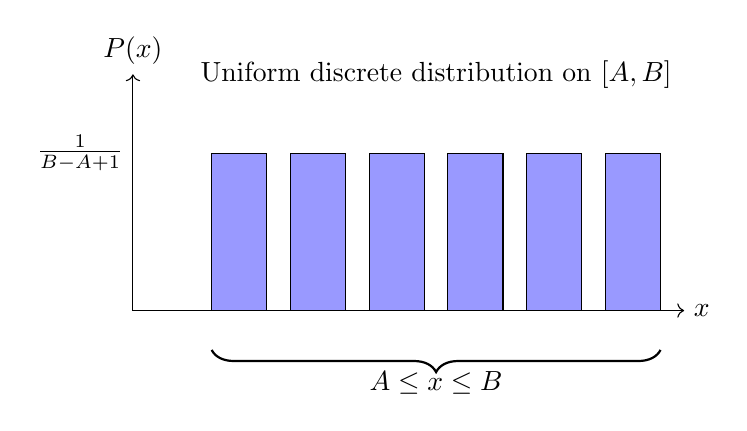
\begin{tikzpicture}
    % Parameters
    \def\a{2}
    \def\b{7}
    \def\n{\b-\a+1}
    \def\height{2}

    % Axes
    \draw[->] (\a-1,0) -- (\b+1,0) node[right] {\(x\)};
    \draw[->] (\a-1,0) -- (\a-1,3) node[above] {\(P(x)\)};

    % Bars for uniform discrete distribution from A to B
    \foreach \x in {\a,...,\b}
      \draw[fill=blue!40] (\x,0) rectangle (\x+0.7,\height);


    % Probability value
    \node[left] at (\a-1,\height) {\(\frac{1}{B-A+1}\)};

    % Title
    \node[above] at ({(\a+\b)/2+0.35},2.7) {Uniform discrete distribution on $[A,B]$};

    % Interval annotation
    \draw[decorate,decoration={brace,amplitude=8pt,mirror},thick] (\a, -0.5) -- (\b+0.7, -0.5) node[midway,below,yshift=-4pt] {\(A \leq x \leq B\)};
  \end{tikzpicture}
  \caption{Uniform discrete distribution over the integers from \(A\) to \(B\)}\label{fig:uniform-discrete-distribution-interval}
\end{figure}

This distribution is used in almost all the random samplings which require a choice from a discrete range of options, such as selecting a predicate from the pool of available ones.
The choice of which logical connective to use instead is made using the discrete distribution given by the \emph{connectives' distribution} parameters. If none of them is specified, the uniform distribution is used instead.

\begin{figure}[H]
  \centering
  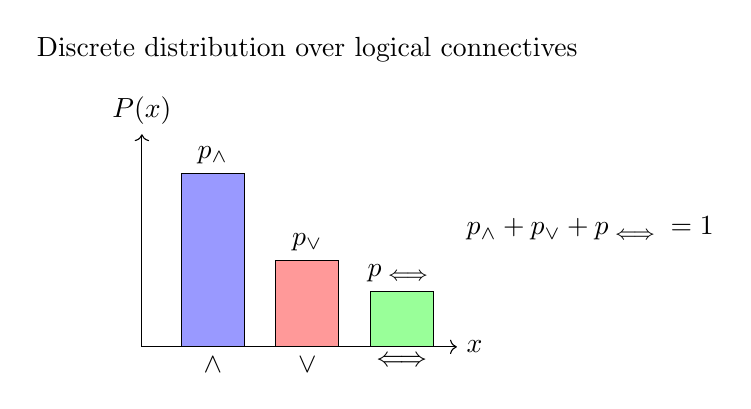
\begin{tikzpicture}
    % Parameters
    \def\heightAnd{2.2}
    \def\heightOr{1.1}
    \def\heightIff{0.7}
    \def\width{0.8}

    % Axes
    \draw[->] (-0.5,0) -- (3.5,0) node[right] {\(x\)};
    \draw[->] (-0.5,0) -- (-0.5,2.7) node[above] {\(P(x)\)};

    % Bars
    \draw[fill=blue!40] (0,0) rectangle (\width,\heightAnd);
    \draw[fill=red!40] (1.2,0) rectangle (1.2+\width,\heightOr);
    \draw[fill=green!40] (2.4,0) rectangle (2.4+\width,\heightIff);

    % Labels below bars
    \node[below] at (0+\width/2,0) {\(\land\)};
    \node[below] at (1.2+\width/2,0) {\(\lor\)};
    \node[below] at (2.4+\width/2,0) {\(\iff\)};

    % Probability values above bars
    \node[above] at (0+\width/2,\heightAnd) {\(p_{\land}\)};
    \node[above] at (1.2+\width/2,\heightOr) {\(p_{\lor}\)};
    \node[above] at (2.4+\width/2,\heightIff) {\(p_{\iff}\)};

    % Title
    \node[above] at (1.2+\width/2,3.5) {Discrete distribution over logical connectives};

    % Sum annotation
    \node[right] at (3.5,1.5) {\(p_{\land} + p_{\lor} + p_{\iff} = 1\)};
  \end{tikzpicture}
  \caption{Example of a discrete probability distribution over logical connectives}\label{fig:connectives-discrete-distribution}
\end{figure}

For binary samplings, such as deciding whether to negate an atomic formula or which quantifier to use, we used the Bernoulli distribution \(\mathcal{B}(p)\), where \(p\) has been fine-tuned for each specific case.

\begin{figure}[H]
  \centering
  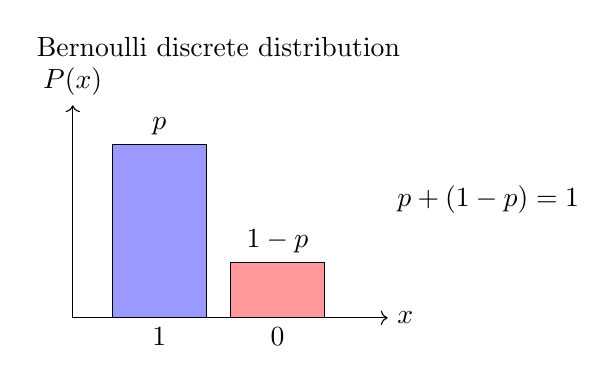
\begin{tikzpicture}
    % Parameters
    \def\width{1.2}
    \def\heightOne{2.2}
    \def\heightZero{0.7}

    % Axes
    \draw[->] (-0.5,0) -- (3.5,0) node[right] {\(x\)};
    \draw[->] (-0.5,0) -- (-0.5,2.7) node[above] {\(P(x)\)};

    % Bars
    \draw[fill=blue!40] (0,0) rectangle (\width,\heightOne);
    \draw[fill=red!40] (1.5,0) rectangle (1.5+\width,\heightZero);

    % Labels below bars
    \node[below] at (0+\width/2,0) {\(1\)};
    \node[below] at (1.5+\width/2,0) {\(0\)};

    % Probability values above bars
    \node[above] at (0+\width/2,\heightOne) {\(p\)};
    \node[above] at (1.5+\width/2,\heightZero) {\(1-p\)};

    % Title
    \node[above] at (0.75+\width/2,3.2) {Bernoulli discrete distribution};

    % Sum annotation
    \node[right] at (3.5,1.5) {\(p + (1-p) = 1\)};
  \end{tikzpicture}
  \caption{Bernoulli discrete distribution with parameter \(p\).}\label{fig:bernoulli-discrete-distribution}
\end{figure}

Lastly, there was another occasion of random sampling not yet covered.
After choosing to generate a binary formula, to increase the variability of the structures of the generated trees, we decided to randomly choose how many symbols to allocate to the left and right subformulae.
This is done by sampling a real coefficient \(c\) from a normal distribution \(\mathcal{N}(\mu, \sigma^2)\) with mean \(\mu = 0.5\) and standard deviation \(\sigma = \frac{1}{18}\), which is then used to proportionally split the available symbols between the two subformulae.
This value of \(\sigma\) was chosen to ensure that the vast majority of the sampled values fall within the range \([\frac{1}{3}, \frac{2}{3}]\), thus avoiding excessively unbalanced splits.
Furthermore, avoiding sampling outside a specified range is mandatory, due to the discrete nature of the length parameter, which would not allow allocating at least one symbol to each subformula.
The natural base case of the recursion, which occurs when the length is \(3\), where the only possible split is 1 symbol for one subformula and 1 for the other, with the remaining symbol being used for the connective.
Being the number of symbols always greater than \(3\) when sampling this coefficient, we can safely use the range \([\frac{1}{3}, \frac{2}{3}]\) for sampling, as it guarantees that both subformulae will always receive at least one symbol.
To achieve this, we implemented a rejection sampling approach, where values outside the specified range are discarded and resampled until a valid value is obtained.
The values of \(\mu\) and \(\sigma\) were chosen to ensure that the vast majority of the sampled values fall within the desired range, thus minimizing the number of rejections and ensuring efficient sampling.

\begin{figure}[H]
  \centering
  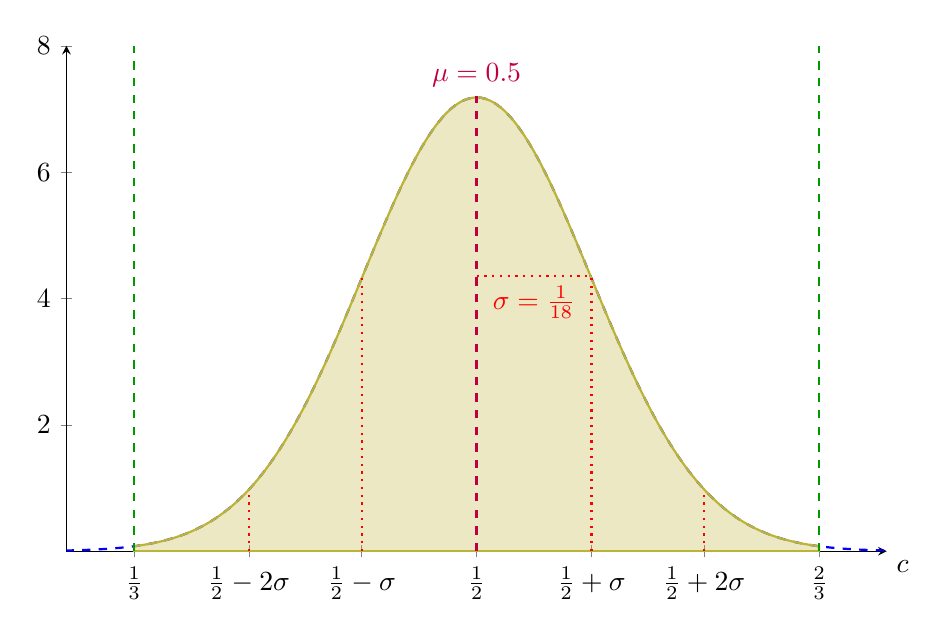
\begin{tikzpicture}
\begin{axis}[
    width=12cm,
    height=8cm,
    axis lines=middle,
    xlabel={$c$},
    xlabel style={at={(axis description cs:1,0)}, anchor=north west},
    ylabel style={at={(axis description cs:0,1)}, anchor=south east, rotate=90},
    xmin=0.3, xmax=0.7,
    ymin=0, ymax=8,
    xtick={0, 0.333,0.389,0.444, 0.5, 0.556, 0.611, 0.667, 1},
    xticklabels={0, $\frac{1}{3}$,$\frac{1}{2}-2\sigma$,$\frac{1}{2}-\sigma$, $\frac{1}{2}$,$\frac{1}{2}+\sigma$,$\frac{1}{2}+2\sigma$, $\frac{2}{3}$, 1},
    ytick={0, 2, 4, 6, 8},
    legend pos=north east,
    title style={font=\large\bfseries}
]

% Distribuzione normale originale (non troncata)
\addplot[
    domain=0:1,
    samples=200,
    smooth,
    thick,
    blue,
    dashed
] {1/sqrt(2*pi*(1/18)^2) * exp(-0.5*((x-0.5)/(1/18))^2)};

% Area troncata (parte accettata)
\addplot[
    domain=0.333:0.667,
    samples=100,
    smooth,
    thick,
    yellow!70!black,
    fill=yellow!70!black,
    fill opacity=0.3
] {1/sqrt(2*pi*(1/18)^2) * exp(-0.5*((x-0.5)/(1/18))^2)} \closedcycle;

% Linee verticali per i limiti di troncamento
\draw[thick, green!60!black,dashed] (axis cs:0.333,0) -- (axis cs:0.333,8);
\draw[thick, green!60!black,dashed] (axis cs:0.667,0) -- (axis cs:0.667,8);

% Linea verticale per la media
\draw[thick, purple, dashed] (axis cs:0.5,0) -- (axis cs:0.5,7.2);

\draw[thick, red, dotted] (axis cs:0.556,0) -- (axis cs:0.556,4.355);
\draw[thick, red, dotted] (axis cs:0.5,4.355) -- (axis cs:0.556,4.355);
\node[anchor=north, red] at (axis cs:0.528, 4.355) {$\sigma = \frac{1}{18}$};
% μ - σ = 0.5 - 1/18 ≈ 0.444  
\draw[thick, red, dotted] (axis cs:0.444,0) -- (axis cs:0.444,4.355);

% μ + 2σ = 0.5 + 2/18 ≈ 0.611
\draw[thick, red, dotted] (axis cs:0.611,0) -- (axis cs:0.611,0.975);
% μ - 2σ = 0.5 - 2/18 ≈ 0.389
\draw[thick, red, dotted] (axis cs:0.389,0) -- (axis cs:0.389,0.975);

% Annotazioni
\node[anchor=south, purple] at (axis cs:0.5, 7.2) {$\mu = 0.5$};


% Legenda

\end{axis}

\end{tikzpicture}
  \caption{Normal distribution \(\mathcal{N}(0.5,\,{(\frac{1}{18})}^2)\) truncated to the interval \([\frac{1}{3}, \frac{2}{3}]\).}\label{fig:truncated-normal-distribution}
\end{figure}


\subsection{Generator Algorithms}\label{subsec:generator-algorithms}

The entry point method of the \code{FlutedGenerator} class is \code{generateProblem}, which generates a fluted problem according to the specified parameters.

\begin{algorithm}[H]
  \caption{Generate fluted problem}\label{alg:generate-fluted-problem}
  \begin{algorithmic}[1]
      \Statex{} \bold{signature} \(\textsc{generateProblem:} \quad Void \to Boolean\)
      \Function{\(\textsc{generateProblem}\)}{$ $} % chktex 46
        \State{} \(unitList \gets \emptyset\)
        \For{\(i \in \{1, \ldots, \_unitsNum\}\)}
          \State{} \(unit \gets generateUnit()\)
          \State{} \(unitList \gets unitList \cup \{unit\}\)
        \EndFor{}
        \State{} \Return{} \(Problem(unitList)\)
      \EndFunction{}
  \end{algorithmic}
\end{algorithm}


Its sole purpose is to call the \code{generateUnit} method the specified number of times, collecting the generated units in a list, and finally returning a \code{Problem} object containing them.
The \code{generateUnit} method is responsible for generating a single fluted \code{FormulaUnit}.
To try to generete more diverse and realistic problems, in this method a random number of usable variables, ranging from 1 to half of the maximum arity specified, is chosen to be quantified in advance.
This is to simulate the common situation in real-world problems where some variables are quantified at the beginning of the formula, as well as allowing proper formula generation to freely even literals from the start, having already some variables available.

\begin{algorithm}[H]
  \caption{Generate fluted unit}\label{alg:generate-fluted-unit}
  \begin{algorithmic}[1]
      \Statex{} \bold{signature} \(\textsc{generateUnit:} \quad Void \to Unit*\)
      \Function{\(\textsc{generateUnit}\)}{$ $} % chktex 46
        \State{} \(varNum \gets uniformRandom(1, \frac{\_maxArity}{2})\)
        \State{} \(usedVars \gets \{0,\ldots,varNum-1\}\)
        \State{} \(formula \gets generateFormula(\_maxLen-varNum, usedVars)\)
        \State{} \(usedVars \gets reverse(usedVars)\)
        \For{\(v \in usedVars\)}
          \State{} \(formula \gets randomlyQuantify(formula, v)\)
        \EndFor{}
        \State{} \Return{} \(FormulaUnit(formula)\)
      \EndFunction{}
  \end{algorithmic}
\end{algorithm}

To handle the generation of a specific type of subformula, being it atomic, binary, or quantified, some helper methods were implemented as follows:

\begin{algorithm}[H]
  \caption{Generate quantified formula}\label{alg:generate-quantified-formula}
  \begin{algorithmic}[1]
      \Statex{} \bold{signature} \(\textsc{randomlyQuantify:} \quad Formula* \times Var \to QuantifiedFormula*\)
      \Function{\(\textsc{randomlyQuantify}\)}{$f, v$} % chktex 46
        \State{} \(varList \gets \{v\}\)
        \If{\(bernoulliTrial(0.5)\)}
          \State{} \(quantifier \gets \exists\)
        \Else{}
          \State{} \(quantifier \gets \forall\)
        \EndIf{}
        \State{} \Return{} \(QuantifiedFormula(quantifier,varList, formula)\)
      \EndFunction{}
  \end{algorithmic}

\end{algorithm}
\begin{algorithm}[H]
  \caption{Generate atomic formula}\label{alg:generate-atomic-formula}
  \begin{algorithmic}[1]
      \Statex{} \bold{signature} \(\textsc{generateAtomicFormula:} \quad VList* \to AtomicFormula*\)
      \Function{\(\textsc{generateAtomicFormula}\)}{$usedVars$} % chktex 46
        \State{} \(arity \gets uniformRandom(1,usedVars)\)
        \State{} \(predIndex \gets uniformRandom(0, \_predNum - 1)\)
        \State{} \(predicate \gets \_predicates[arity-1] [predIndex]\)
        \State{} \(litVars \gets selectLastN(usedVars, arity)\)
        \State{} \(isNegated \gets bernoulliTrial(0.5)\)
        \State{} \(l \gets Literal(predicate, arity, isNegated,litVars)\)
        \State{} \Return{} \(AtomicFormula(l)\)
      \EndFunction{}
  \end{algorithmic}
\end{algorithm}
\begin{algorithm}[H]
  \caption{Generate binary formula}\label{alg:generate-binary-formula}
  \begin{algorithmic}[1]
      \Statex{} \bold{signature} \(\textsc{generateBinaryFormula:} \quad Unsigned \times VList* \to Formula*\)
      \Statex{} \textbf{require} \(len > 3\)
      \Function{\(\textsc{generateBinaryFormula}\)}{$len, usedVars$} % chktex 46
        \State{} \(connective \gets generateConnective()\)
        \Comment{Sampled from \emph{connectives' distribution}}
        \State{} \(remLen \gets len - 1\)
        \State{} \(c \gets truncatedNormalRandom(0.5, \frac{1}{18}, \frac{1}{3}, \frac{2}{3})\)
        \State{} \(leftLen \gets round(c \cdot remLen)\)
        \State{} \(rightLen \gets remLen - leftLen\)
        \State{} \(leftFormula \gets generateFormula(leftLen, usedVars)\)
        \State{} \(rightFormula \gets generateFormula(rightLen, usedVars)\)
        \If{\(connective = \iff\)}
          \State{} \Return{} \(BinaryFormula(\iff,leftFormula, rightFormula)\)
        \Else{}
          \State{} \Return{} \(JunctionFormula(connective,\{leftFormula, rightFormula\})\)
        \EndIf{}
      \EndFunction{}
  \end{algorithmic}
\end{algorithm}

Finally, the \code{generateFormula} method orchestrates the recursive generation of the formula, deciding at each step which type of subformula to generate based on the remaining length and the available variables.
To chose if generating a quantified formula or not, we used a Bernoulli distribution with \(p\) dynamically adjusted with the function
\[
p_{quantify} = \min\left(\frac{\_maxArity - |usedVars|}{remainingLength - 1}, 1\right)
\]
\begin{figure}[H]
\centering
\begin{minipage}{0.48\textwidth}
\centering
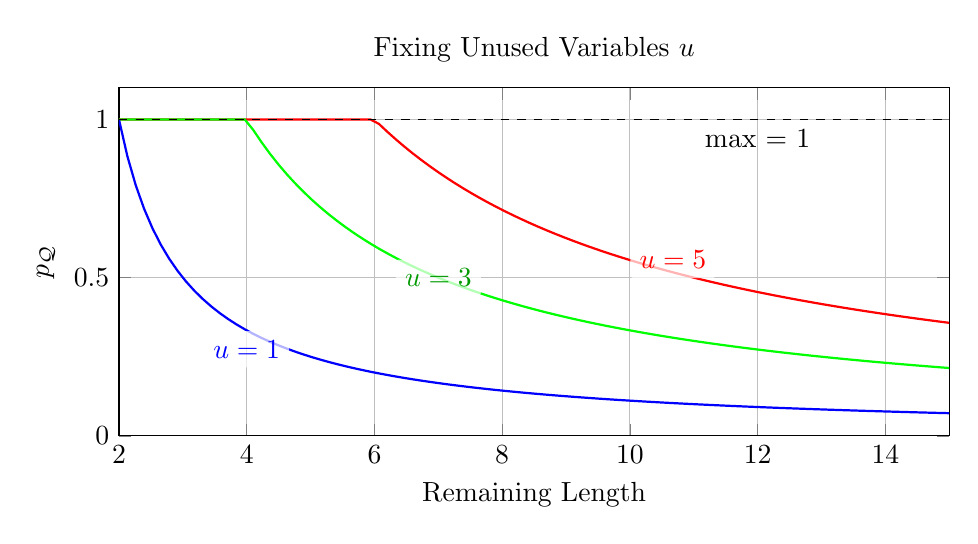
\begin{tikzpicture}
\begin{axis}[
    xlabel={Remaining Length},
    ylabel={$p_{\mathcal{Q}}$},
    xmin=2, xmax=15,
    ymin=0, ymax=1.1,
    grid=major,
    width=\textwidth,
    height=6cm,
    samples=100,
    title={Fixing Unused Variables \(u\)}
]

\addplot[red, thick, domain=2:15] {min(5/(x-1), 1)};
\addplot[green, thick, domain=2:15] {min(3/(x-1), 1)};
\addplot[blue, thick, domain=2:15] {min(1/(x-1), 1)};
\addplot[black, dashed, domain=2:15] {1};

\node[blue, anchor=north, fill=white, fill opacity=0.7, text opacity=1, rounded corners=1pt] at (axis cs:4, 0.333) {\(u = 1\)};
\node[green!60!black, fill=white, fill opacity=0.7, text opacity=1, rounded corners=1pt] at (axis cs:7, 0.5) {\(u = 3\)};
\node[red, anchor=west, fill=white, fill opacity=0.7, text opacity=1, rounded corners=1pt] at (axis cs:10, 0.556) {\(u = 5\)};
\node[black, anchor=north] at (axis cs:12, 1) {max = 1};

\end{axis}
\end{tikzpicture}

\end{minipage}
\hfill
\begin{minipage}{0.48\textwidth}
\centering
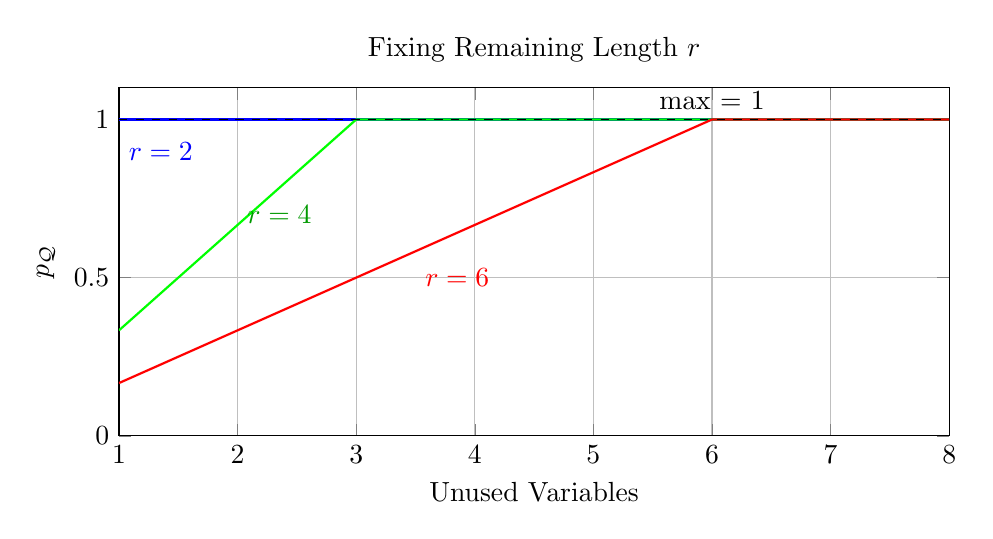
\begin{tikzpicture}
\begin{axis}[
    xlabel={Unused Variables},
    ylabel={$p_{\mathcal{Q}}$},
    xmin=1, xmax=8,
    ymin=0, ymax=1.1,
    grid=major,
    width=\textwidth,
    height=6cm,
    samples=100,
    title={Fixing Remaining Length \(r\)}
]

\addplot[blue, thick, domain=1:10] {min(x/1, 1)};
\node[blue, anchor=west] at (axis cs:1, 0.9) {\(r = 2\)};

\addplot[green, thick, domain=1:10] {min(x/3, 1)};
\node[green!60!black, anchor=west] at (axis cs:2, 0.7) {\(r = 4\)};


\addplot[red, thick, domain=1:10] {min(x/6, 1)};
\node[red, anchor=west] at (axis cs:3.5, 0.5) {\(r = 6\)};

\addplot[black, dashed, domain=1:10] {1};
\node[black, anchor=south] at (axis cs:6, 1) {max = 1};

\end{axis}
\end{tikzpicture}

\end{minipage}
\caption{Behaviour of \(p_{\mathcal{Q}}\) with fixed unused variables (left) and fixed remaining length (right).}\label{fig:pquantify}
\end{figure}

This function ensures that the probability of quantifying a new variable increases as the density of quantification in the formula decreases, thus promoting a balanced distribution of quantifiers throughout the formula.

Finally, the \code{generateFormula} method is as follows:
\begin{algorithm}[H]
  \caption{Generate fluted formula}\label{alg:generate-fluted-formula}
  \begin{algorithmic}[1]
      \Statex{} \bold{signature} \(\textsc{generateFormula:} \quad Unsigned \times VList* \to Formula*\)
      \Statex{} \textbf{require} \(len \geq 3\)
      \Function{\(\textsc{generateFormula}\)}{$len, usedVars$} % chktex 46
        \If{\(len = 1\)}
          \State{} \Return{} \(generateAtomicFormula(usedVars)\)
        \EndIf{}
        \State{} \(varNum \gets |usedVars|\)
        \If{\(varNum \geq \_maxArity\)}
        \Comment{No quantification possible}
          \If{\(len = 2\)}
            \Comment{Cannot generate binary formula}
            \State{} \Return{} \(generateAtomicFormula(usedVars)\)
          \EndIf{}
        \Else{}
          \State{} \(p_{\mathcal{Q}} \gets \min\left(\frac{\_maxArity - varNum}{len - 1}, 1\right)\)
          \If{\(bernoulliTrial(p_{\mathcal{Q}})\)}
            \Comment{Generate quantified formula}
            \State{} \(usedVars \gets usedVars \cup \{varNum\}\)
            \State{} \(subFormula \gets generateFormula(len - 1, usedVars)\)
            \State{} \Return{} \(randomlyQuantify(subFormula, varNum)\)
          \EndIf{}
        \EndIf{}
        \If{\(bernoulliTrial(0.1)\)}
          \Comment{Rare premature atomic formula generation}
          \State{} \Return{} \(generateAtomicFormula(usedVars)\)
        \Else{}
          \Comment{Generate binary formula}
          \State{} \Return{} \(generateBinaryFormula(len, usedVars)\)
        \EndIf{}
      \EndFunction{}
  \end{algorithmic}
\end{algorithm}

Due to time constraints, we decided to limit the generation to unsatisfiable problems only, to have easier and more reliable means of verifying the correctness of the implementation, allowing for more controlled testing conditions.
To achieve this, we implemented a simple strategy: for each generated problem, a random unit is selected, and its negation is added to the problem as an additional unit.

To have more variety and to try to decrease the instant resolutions, we considered the possibility of altering the unit to be negated before adding it to the list, substituting a section of the initial sequence of quantifiers with existential quantifiers.
However, this idea was not implemented in the current work, and we leave it as a direction for future improvements and experiments.
\section{Generation Parameters}\label{sec:generation-parameters}

To conduct a systematic benchmarking study, we had to decide which generation parameters could significantly impact the performance of the decision procedures and therefore should be varied during the experiments.
Other than this, we also had to choose appropriate ranges for these parameters, balancing the need for diversity in the generated problems with the practical constraints of computational resources and time.
After careful consideration, we identified the following key parameters to vary:
\begin{itemize}
\item \textbf{Maximal arity} (\code{_maxArity}):  This parameter is fundamental, as it directly controls the maximum number of variables \(m\) that can appear in a generated formula.
                                                  Since the satisfiability problem for the fluted fragment is known to have \emph{non-elementary complexity} in \(m\)~\cite{pratt2019fluted}, with the fluted formula over \(m\) variables being
                                                   \(\lfloor \frac{m}{2} \rfloor-\textsc{NExpTime}\)-hard and requiring models of \((\frac{m}{2})\)-tuply exponential size, \code{_maxArity} is expected to have a significant impact on performance.
                                                  We chose to vary this parameter from \(2\) to \(15\), to cover a wide range of complexities while keeping the generated problems manageable for testing.
\item \textbf{Maximal length} (\code{_maxLen}): This parameter controls the size of the generated formulae, which can affect both the preprocessing time and the saturation time.
                                                Moreover, longer formulae can lead to a larger number of clauses after clausification, potentially increasing the search space for the resolution procedure.
                                                On the other hand, increasing the number of clauses produced can also provide more opportunities for contradictions to be generated, which could potentially aid in finding a refutation.
                                                We decided to vary this parameter from \(10\) to \(30\) with increments of \(5\).
\item \textbf{Predicates number} (\code{_predNum}): This parameter influences the diversity of predicates in the generated formulae.
                                                  A higher number of distinct predicates can lead to fewer opportunities for unification during resolution, potentially increasing the difficulty of the problem.
                                                  We chose to vary this parameter from \(1\) to \(10\) to observe its effect on performance.
\item \textbf{Units number} (\code{_unitsNum}): This parameter determines the number of units in the generated problem.
                                                Similarly to the maximal length, increasing the number of units can lead to a larger search space, but also more opportunities for contradictions.
                                                We decided to vary this parameter from \(1\) to \(10\) with gaps of \(3\).
\item \textbf{Connectives' distribution} (\code{_iffProb}): As shown in Section~\ref{sec:tptp-results-analysis}, the presence of biconditionals can significantly affect the performance of the fluted preprocessing and resolution.
                                                            To study this effect, we decided to vary the probability of generating biconditionals (and consequently the probabilities of generating conjunctions and disjunctions) in the generated formulae.
                                                            We chose to have three different options for this parameter: \(\frac{1}{3}\), \(\frac{2}{5}\), and \(\frac{1}{2}\), with the remaining probability mass distributed uniformly between conjunctions and disjunctions.

\end{itemize}
\subsection{Gradual difficulty escalation}\label{subsec:gradual-difficulty-escalation}

Combining all the variations of the selected parameters would lead to a total of \(14 \times 5 \times 10 \times 4 \times 3 = 8400\) different configurations.
To add more robustness to the experiments, we decided to generate \(25\) instances for each configuration, leading to a total of \(210000\) generated problems.

With so many problems to test, it was crucial to have a systematic approach to manage how parameters were varied to avoid growing the complexity of the problems too quickly on one axis while neglecting others.
Iterating through all the combinations in a naive way could lead to situations where some parameters were increased too rapidly, resulting in problems that were too difficult to solve within the time limits, while others remained too easy.
To address this, we implemented a gradual difficulty escalation strategy, where parameters were increased in a controlled manner.

First, we identified the parameters that we expected to have the least impact on the complexity of the problems: \code{_predNum}, \code{_maxLen}, and \code{_unitsNum}.
Those three parameters were grouped together, and their combinations were iterated through in a nested manner.
In particular, these three parameters were encoded in three dimensions using a lexicographic ordering, with \code{_predNum} as the most significant dimension, \code{_maxLen} as the middle dimension, and \code{_unitsNum} as the least significant (i.e., the one that changes most rapidly).
In other words, the larger the domain of a parameter, the more slowly it was made to change, ensuring that variations in \code{_predNum} and \code{_maxLen} occur more gradually.
This strategy was chosen to provide immediate diversity in the generated instances, so that changes in the faster-varying parameter (\code{_unitsNum}) do not wait for a complete cycle of \code{_predNum} values (which has 10 possible values).

As mentioned above, variations in maximum arity were expected to have the most significant impact on problem complexity, so we opted to vary this parameter at the same rate as the combination of the previous 3.
For doing so, we encoded the values of the previous 3 parameters into a single index \(i\) ranging from \(0\) to \(199\) (the total number of combinations of the three parameters) using the formula
\[i = \text{\code{_predNum}} + \text{\code{_maxLen}} \times 4 + \text{\code{_unitsNum}} \times 20\]
Then, being \code{_maxArity} ranging from \(2\) to \(15\), we grouped the values of \(i\) into \(14\) groups, \(13\) of them containing \(15\) values and the last one containing \(5\) values.
Having now two equipotent sets of values, we could easily use Cantor's pairing function to combine them into a single index.
\[\pi(i, j) = \frac{(i + j)(i + j + 1)}{2} + j\]
This encoding ensures that as we iterate through the natural number, these can be decoded back into a pair of values \((i, j)\) that change in a balanced manner, thus achieving the desired gradual escalation of difficulty across all parameters.

\begin{figure}[H]
  \centering
  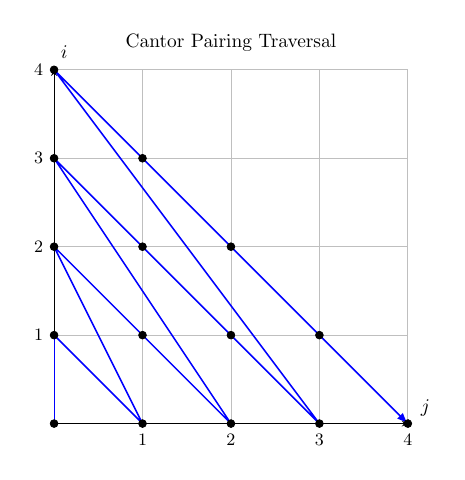
\begin{tikzpicture}[scale=0.7, transform shape]
    \begin{axis}[
      width=8cm,
      height=8cm,
      axis lines=middle,
      xlabel={$i$},
      ylabel={$j$},
      xlabel style={at={(axis description cs:0,1.05)}, anchor=west}, % etichetta x in alto
      ylabel style={at={(axis description cs:1.05,0)}, anchor=south},  % etichetta y a destra
      xmin=0, xmax=4,
      ymin=0, ymax=4,
      xtick={0,1,2,3,4},
      ytick={0,1,2,3,4},
      grid=both,
      minor tick num=0,
      tick label style={font=\small},
      title={Cantor Pairing Traversal}
    ]
      % Traversal arrows
      \addplot[thick, blue, -{Latex[length=2mm]}, mark=none] coordinates {
        (0,0) (0,1) (1,0) (0,2) (1,1) (2,0) (0,3) (1,2) (2,1) (3,0) (0,4) (1,3) (2,2) (3,1) (4,0)
      };

    \foreach \s in {0,...,4} {
      \foreach \k in {0,...,4} {
        \pgfmathsetmacro{\i}{\k}
        \pgfmathsetmacro{\j}{\s-\k}
        \pgfmathsetmacro{\cantor}{(\i+\j)*(\i+\j+1)/2+\j}
        \addplot[ only marks] coordinates {(\i,\j)};
      }
    }
    \end{axis}
    % Cantor pairing traversal (diagonals) con etichette

  \end{tikzpicture}
  \caption{Traversal order of the Cantor pairing function: diagonal progression \((0,0)\to(0,1)\to(1,0)\to(0,2)\to(1,1)\to(2,0)\to\cdots\) on the \(i,j\) plane.}\label{fig:cantor-pairing-diagonal}
\end{figure}

Finally, the probability of generating biconditionals was varied at the slowest rate, changing only after a complete cycle of the previous 4 parameters.

\section{Experimental Setup, Results and Analysis}\label{sec:results-analysis}

For the generated problems testing, we used a similar experimental setup to the one used for the TPTP problems, with some differences.
The hardware used for the tests was the same as described in Section~\ref{sec:tptp-experimental-setup}, as well as time limit of \(300\) seconds per problem and the symbolic value of \(330\) for problems which led to an error.

For measuring the impact of the preprocessing step, we decided to include a new hybrid execution mode, where the fluted preprocessing is applied, but the resulting clauses are then passed to the standard non-fluted resolution procedure.
This hybrid mode allows us to isolate the effect of the preprocessing step from the fluted-specific optimizations in the resolution procedure, providing a clearer picture of where the performance gains are coming from.

As for the resolution strategy, in this case we limited ourselves to the \emph{LRS} strategy, since its performance are typically better. Its incompleteness is not a concern here, as we are only dealing with unsatisfiable problems.
In any case, all the problems that resulted satisfiable by the LRS strategy were flagged as errors, and accumulated in a log for future further analysis.

Testing all the huge number of generated problems we aimed to test (\(210000 \times 3\) modes = \(630000 \times 5\) runs = \(3150000 \times 5\) potential minutes = \(15750000\) minutes), was simply not feasible as it would have required potentially nearly 30 years of continuous computation.
To make the experiments manageable, we decided to do multiple runs only to problems that took less than \(30\) seconds in the first run, where possible hardware or software fluctuations could have a more significant impact on the measured time.
Moreover, after some initial experimentation that highlighted the fact that the timeout of hybrid mode and Vampire mode were very similar, we decided to skip Vampire mode for problems that reached the timeout in hybrid mode, as they were very likely to also timeout in Vampire mode.
For those problems, a symbolic value of \(400\) seconds was assigned to Vampire mode for charts, while a value of \(300\) seconds was assigned when calculating aggregated results.

Although the tests have performed at any time possible for over two months, we managed to complete only the first \(75/200\) numbers of lexicographic encoding for the first \(8/14\) variables, never changing the value of \code{_iffProb} from \(\frac{1}{3}\).
This resulted in a total of \(15000\) generated problems, which were tested in all three modes, leading to a total of \(45000\) tests, potentially with \(5\) runs each.
The full set of results was too large to be included in this document, so we uploaded it to a public repository\footnote{\url{https://github.com/RiccardoElena/thesis_benchmarks}}.
Even reporting charts similar to those in Section~\ref{sec:tptp-results-analysis} with all problems on the x-axis would be impossible due to the sheer number of problems.
Therefore, after showing some examples of charts for specific configurations, we will focus on aggregated results, which can provide a more concise overview highlighting the main trends and differences between the execution modes.

The first set of charts we present are examples of specific configurations, and they exhibit similar patterns to those observed in the TPTP results.
In particular, we can see that the fluted mode of consistently outperforms the vampire mode, with the hybrid mode often being very close to the fluted mode, indicating that the preprocessing step is a significant contributor to the performance improvement.

\begin{figure}[H]
  \centering
  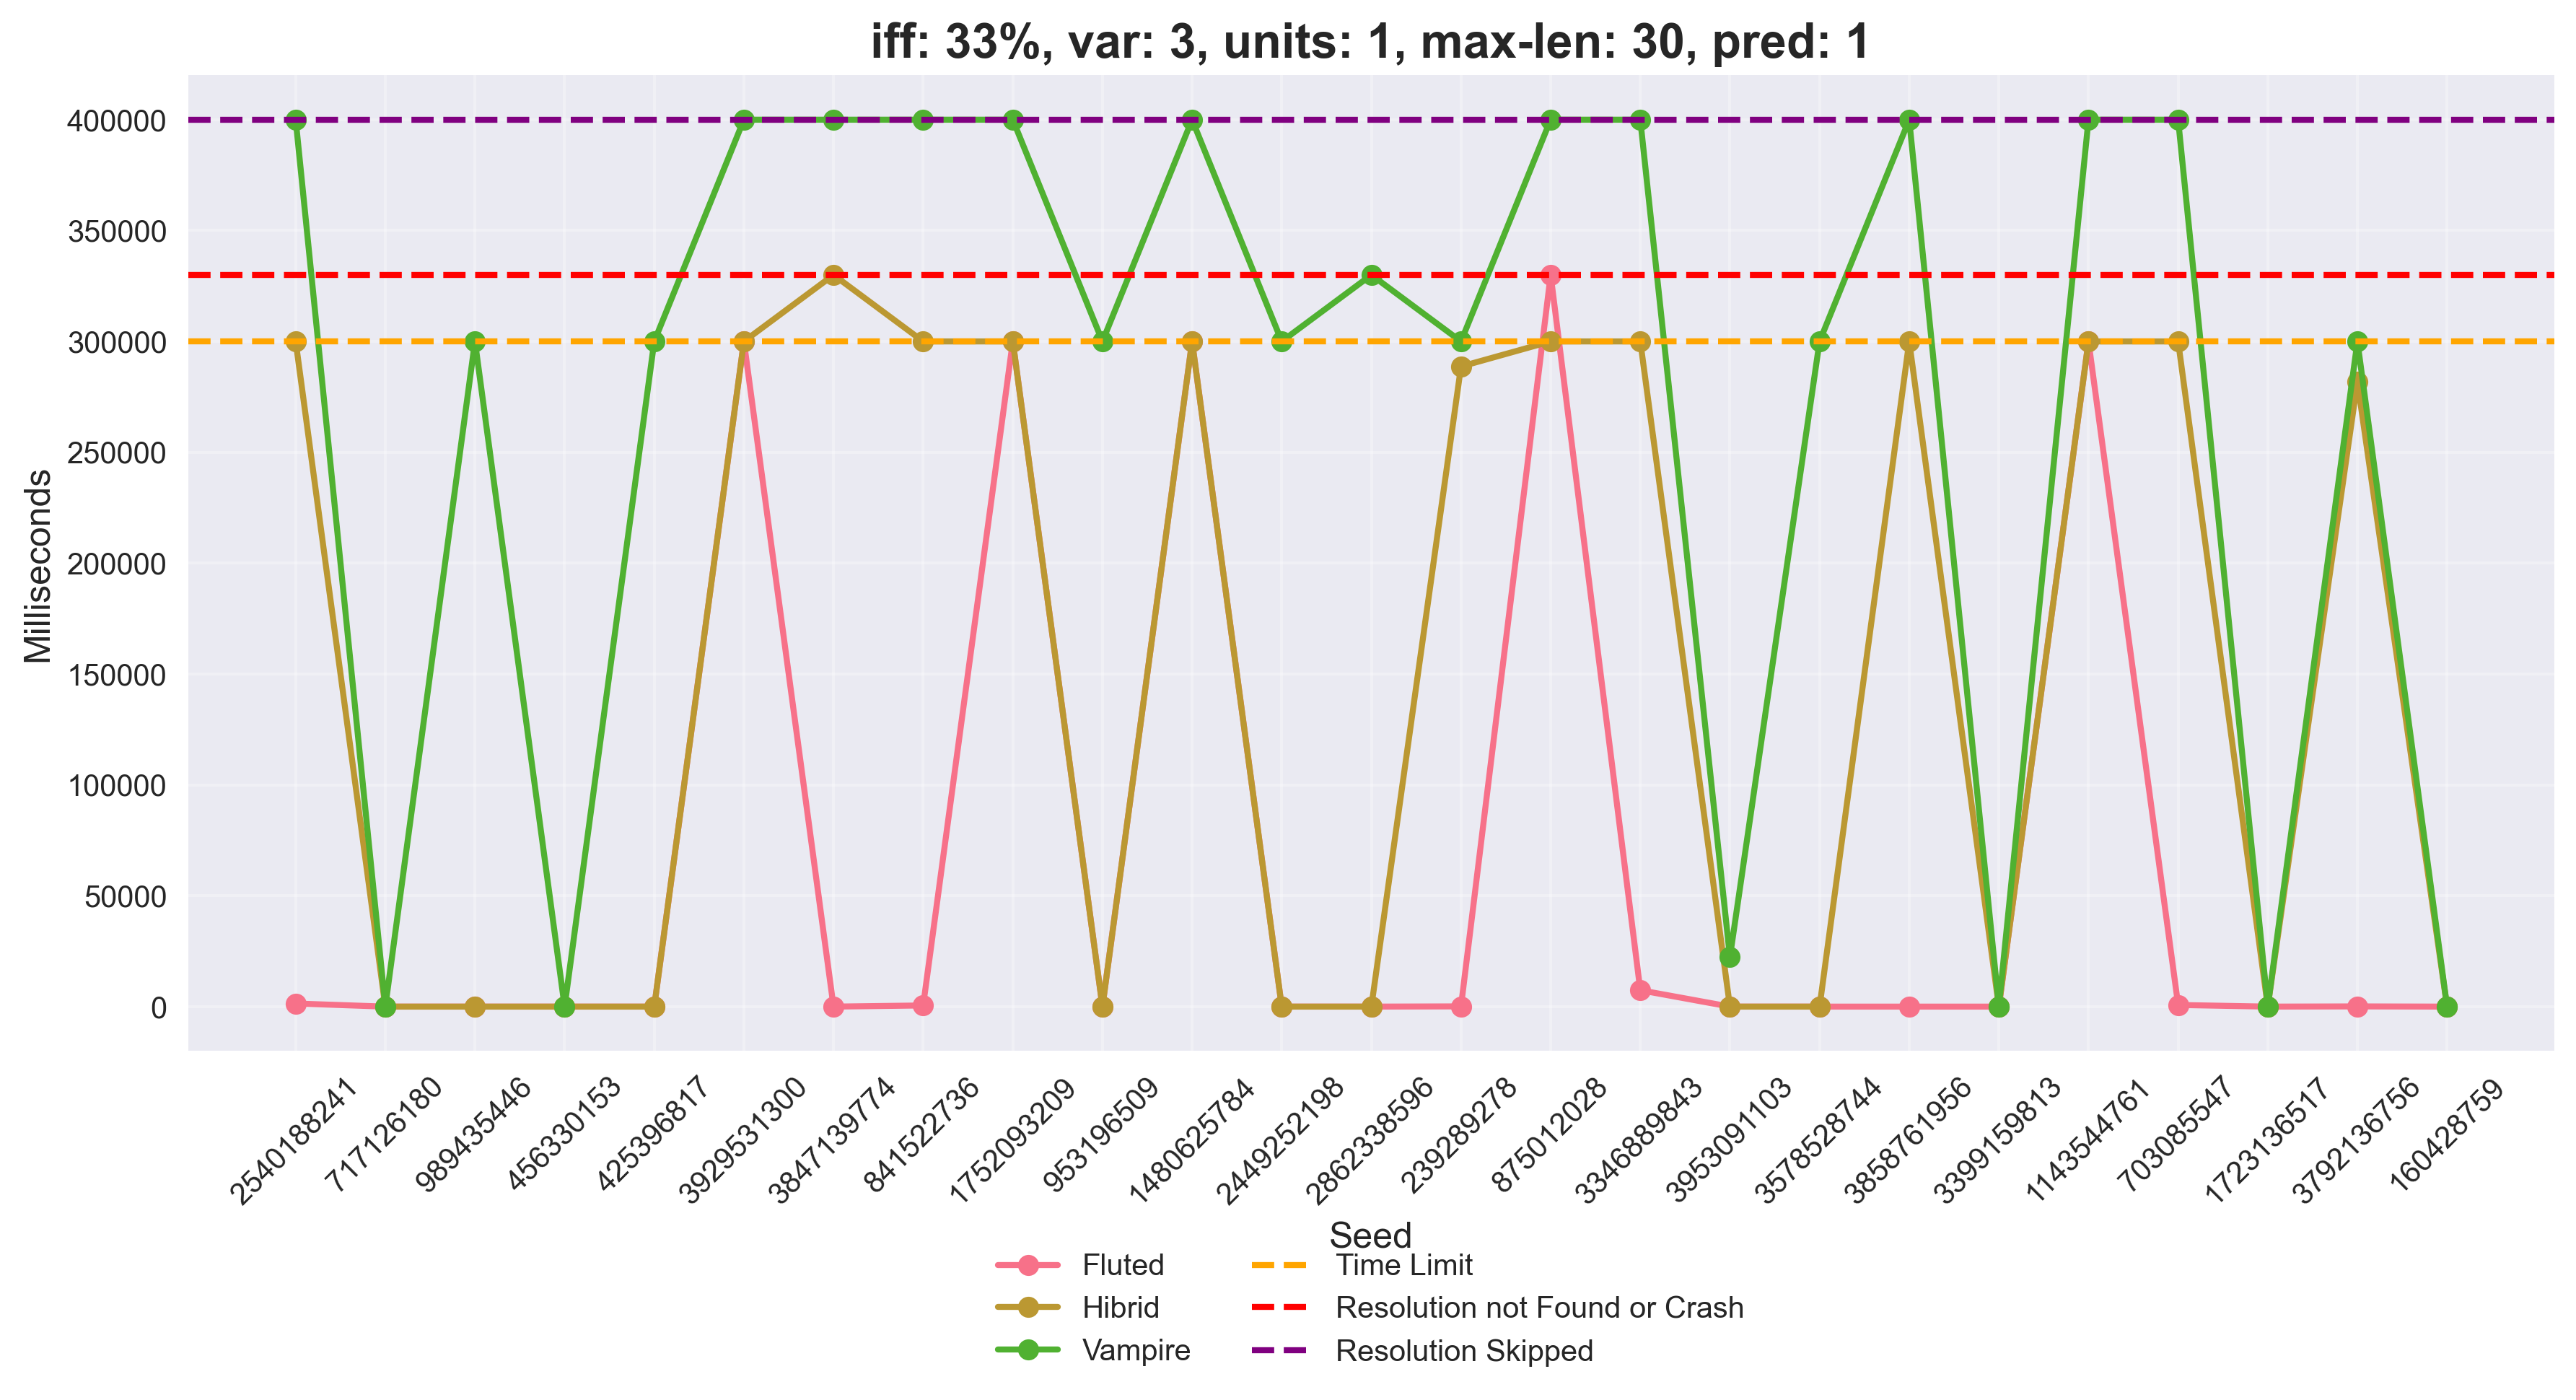
\includegraphics[width=\textwidth]{7-generated-benchmarking/singles/res-16_linee_normal.png}
\end{figure}
\begin{figure}[H]
    \centering
    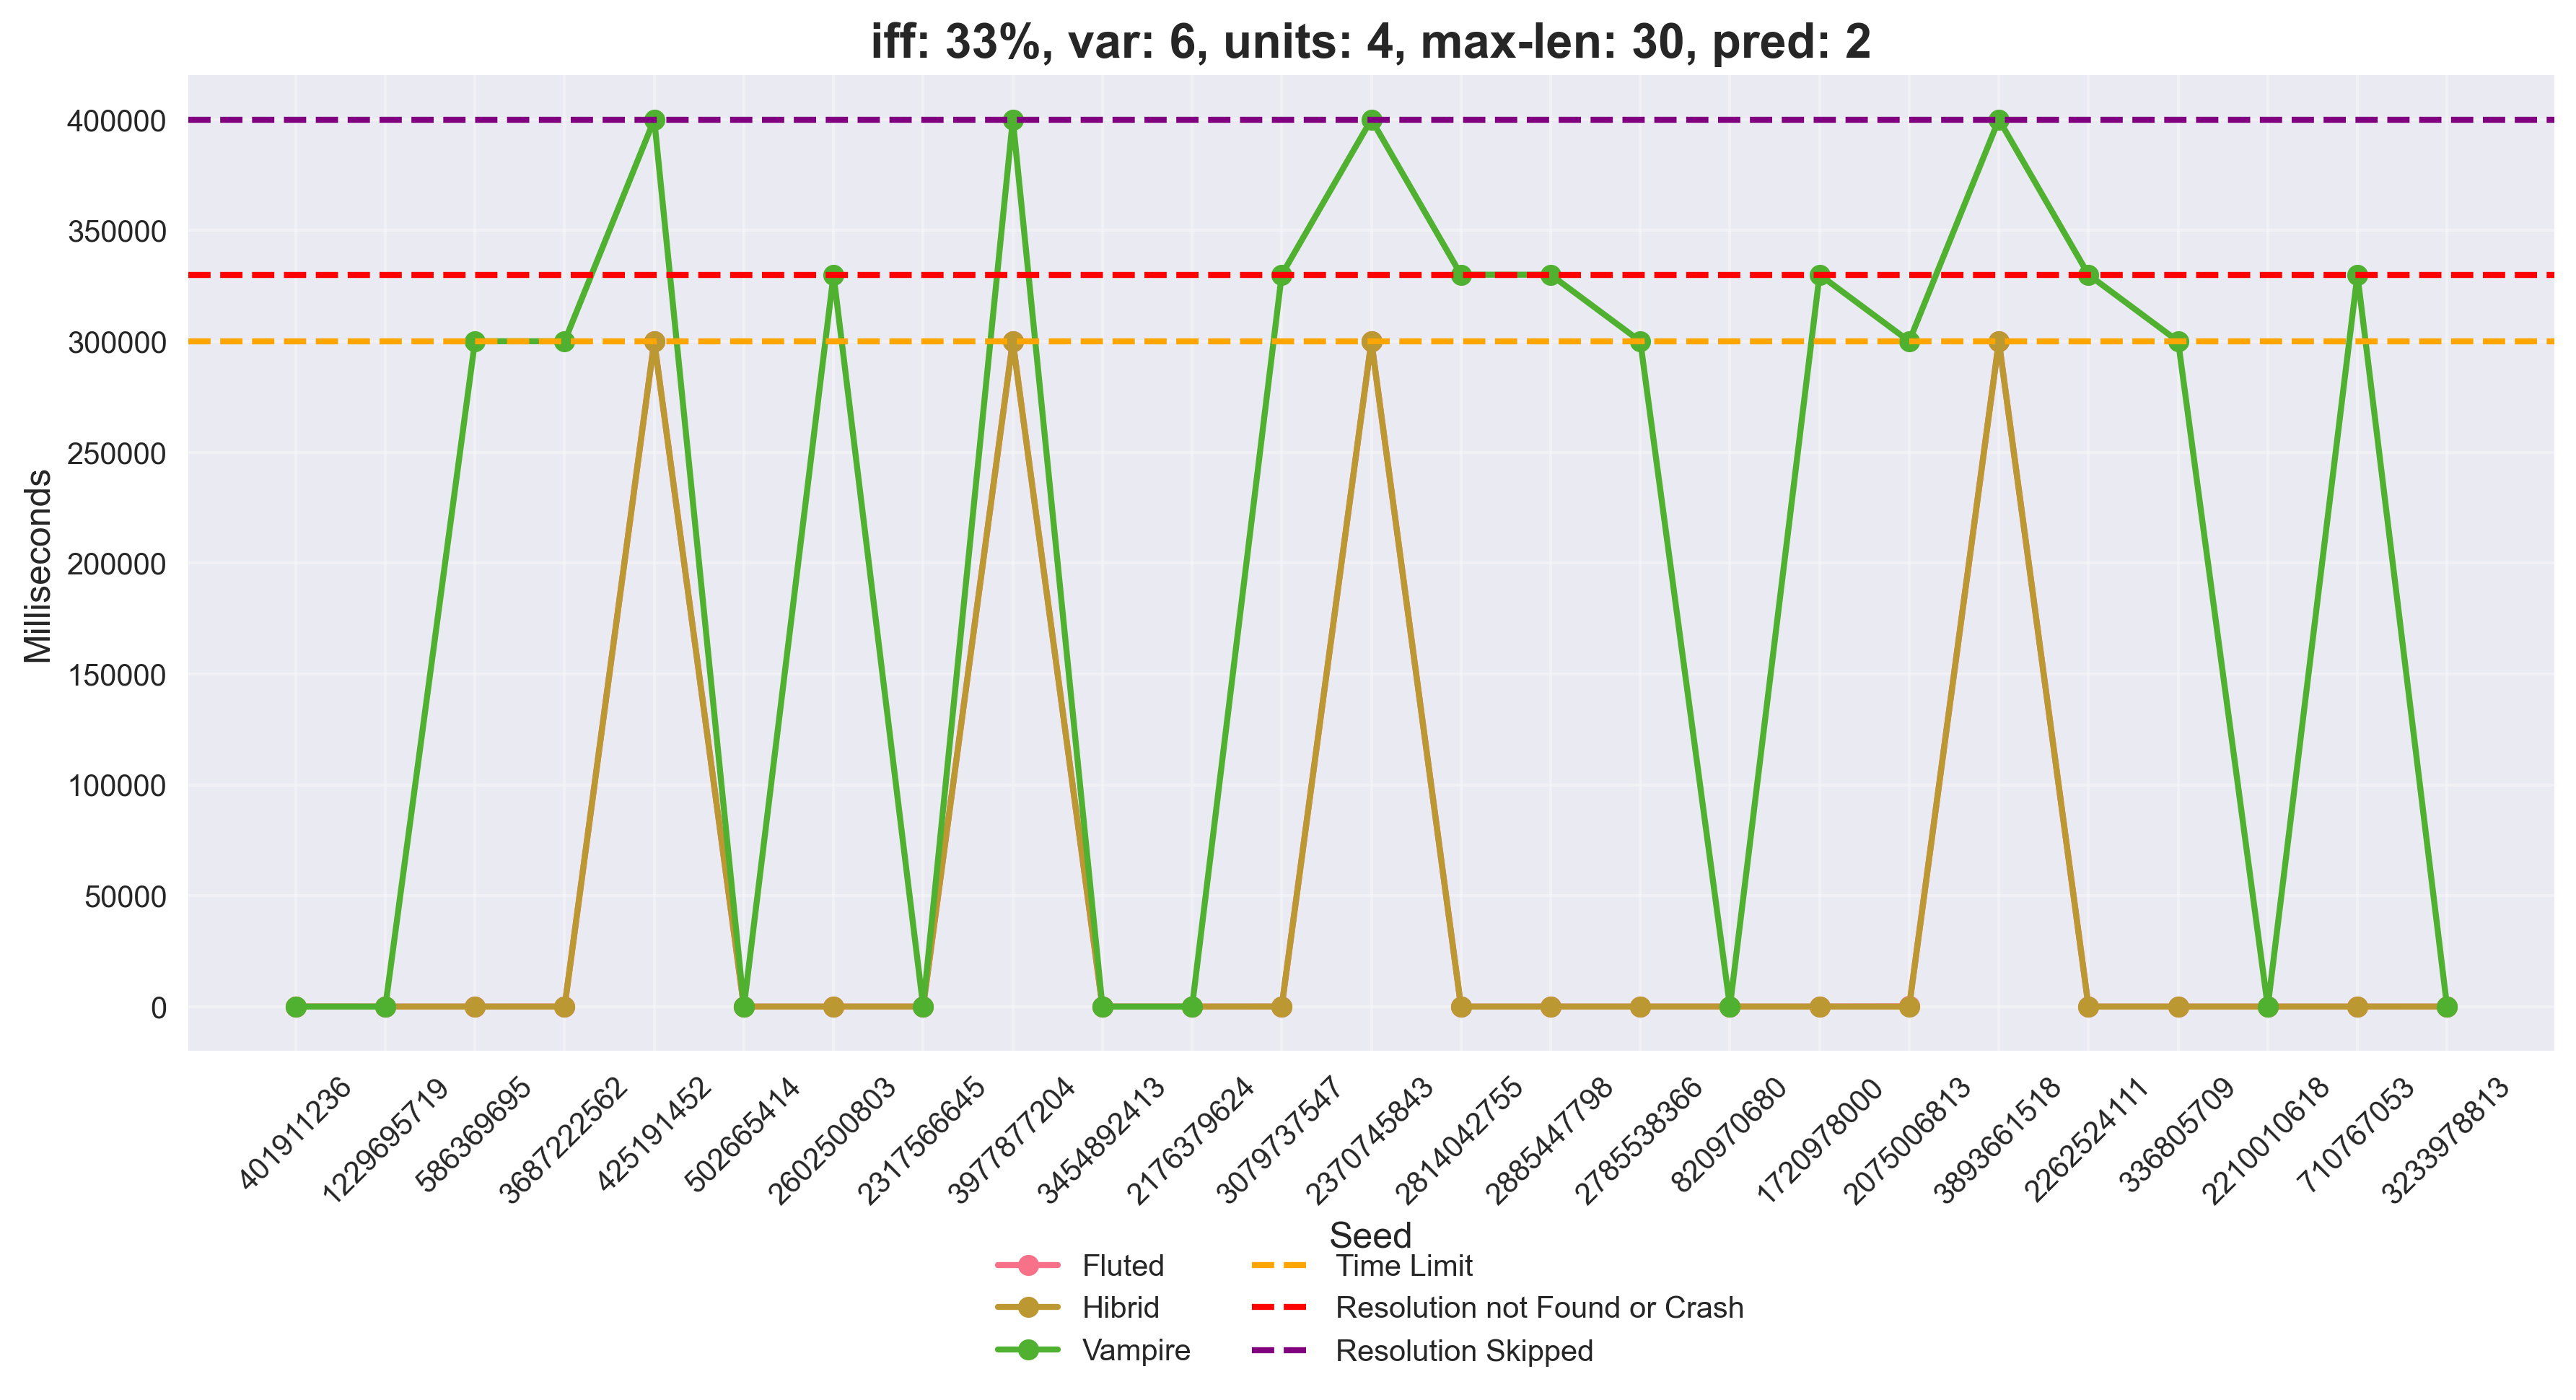
\includegraphics[width=\textwidth]{7-generated-benchmarking/singles/res-37_linee_normal.png}
\end{figure}
\begin{figure}[H]
    \centering
    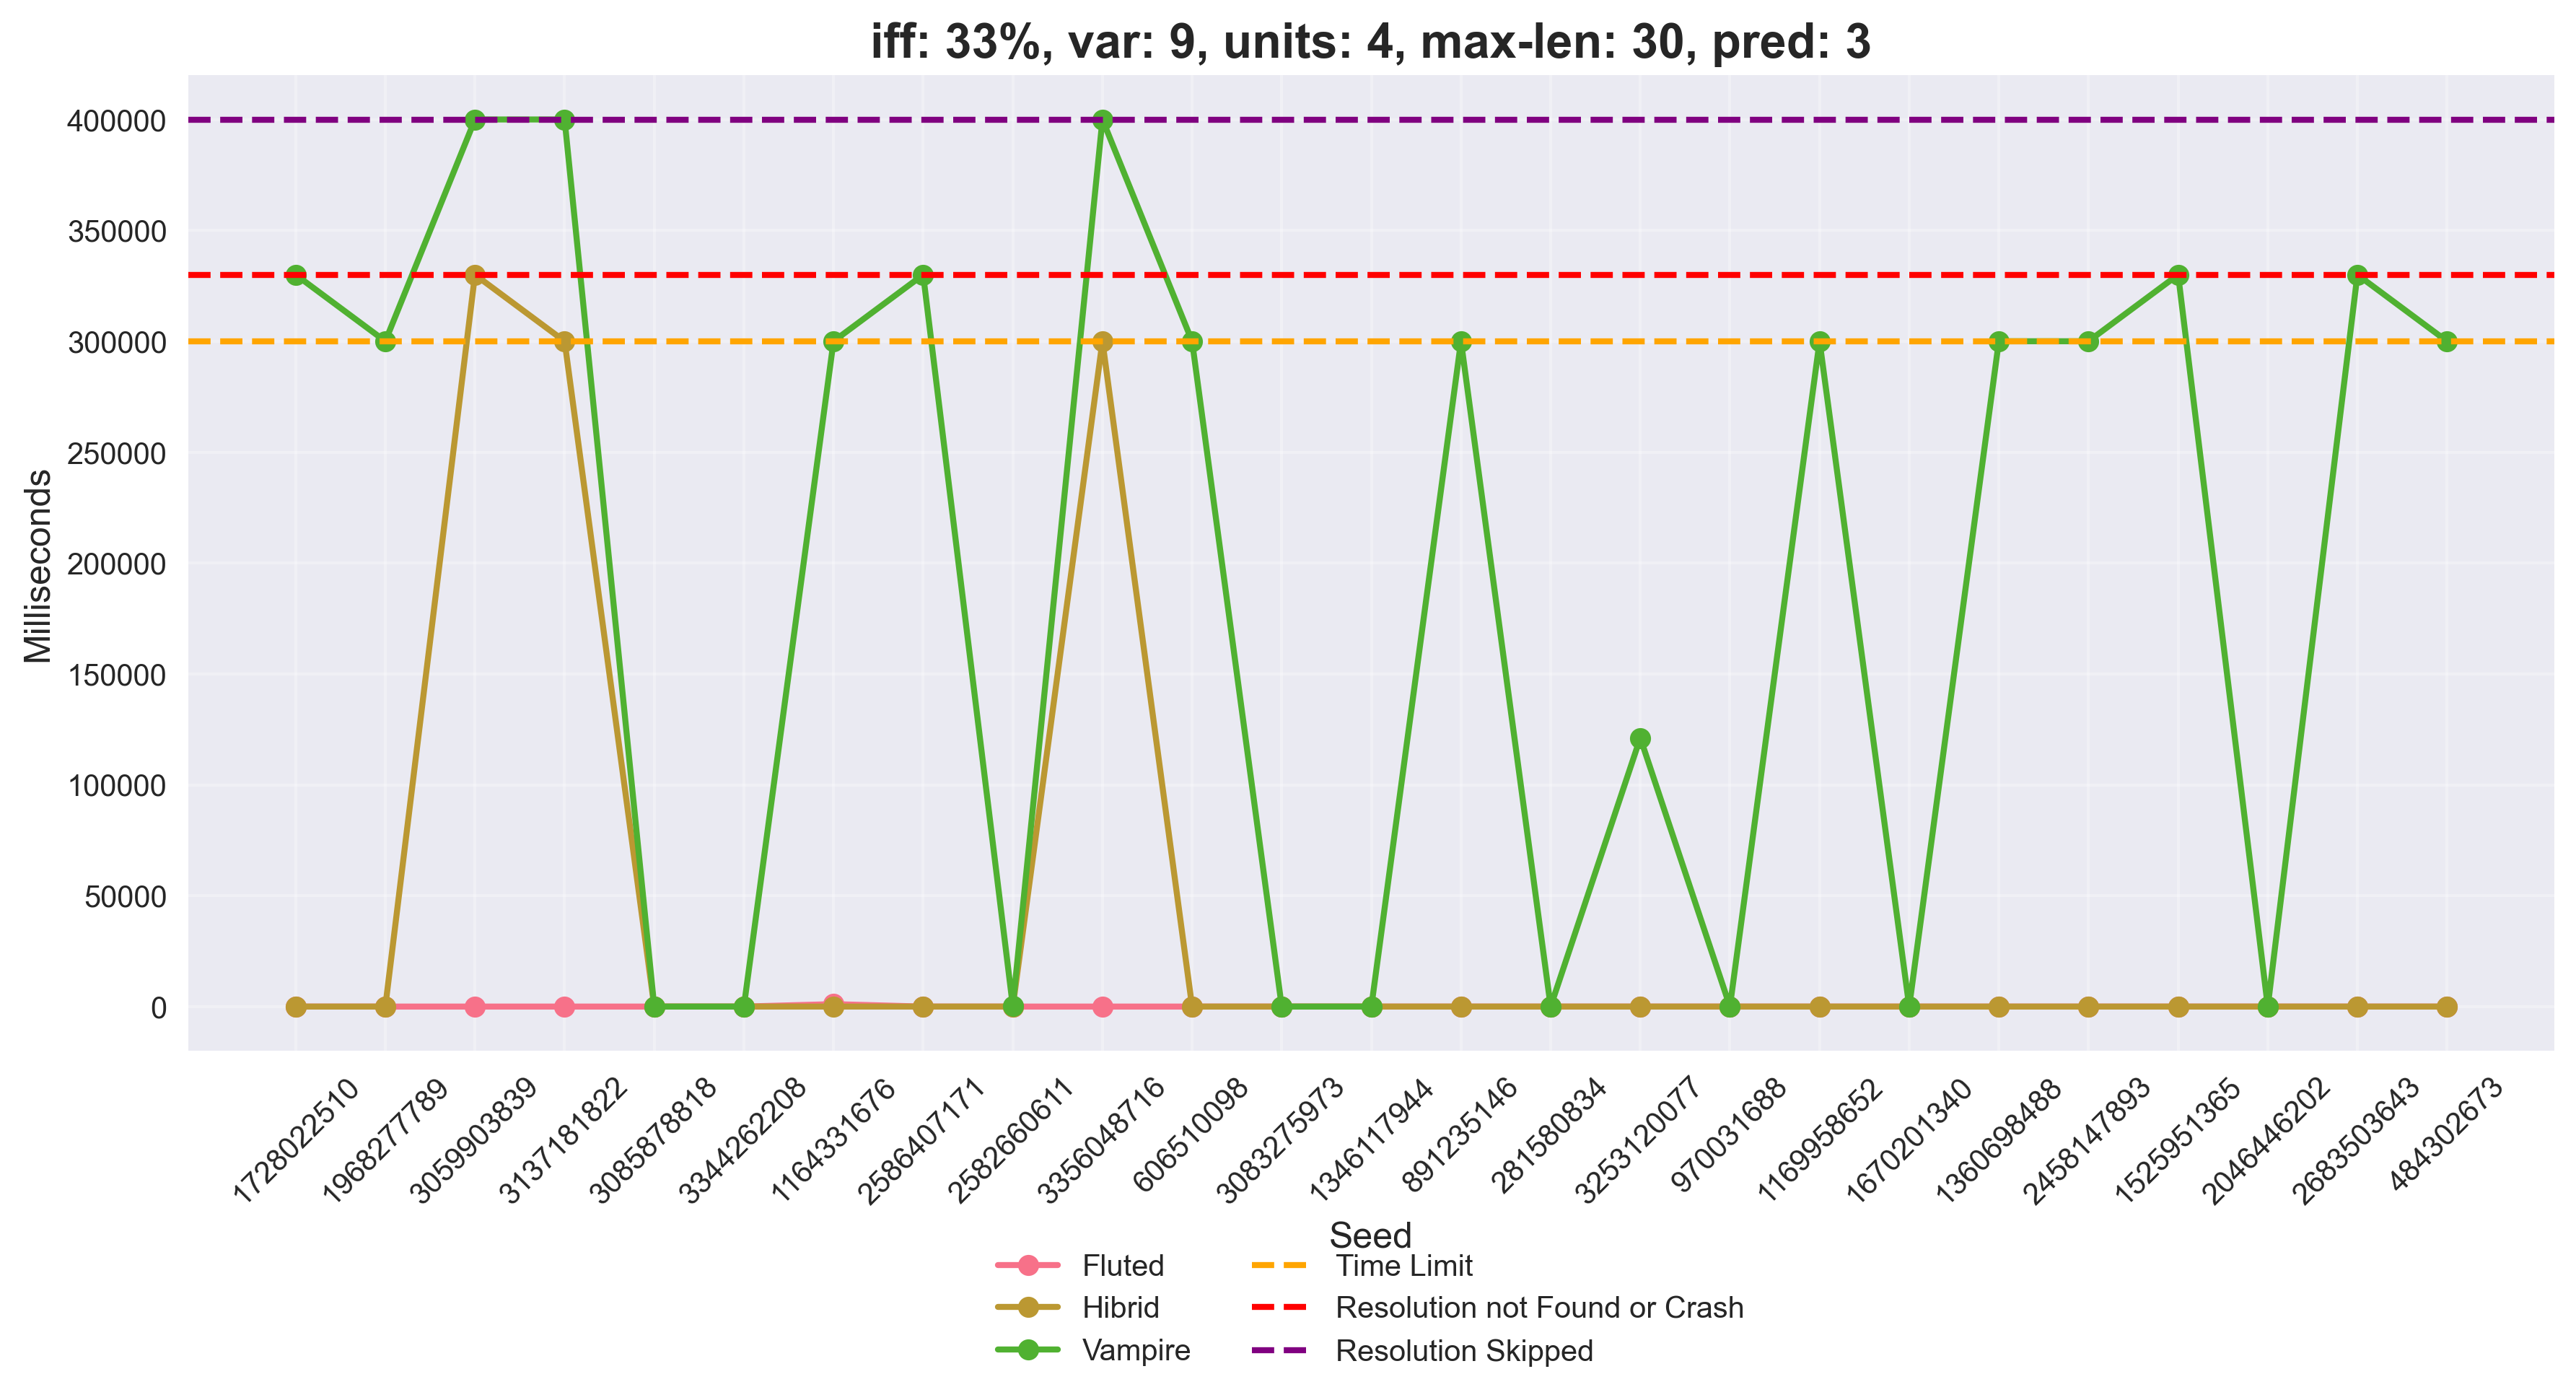
\includegraphics[width=\textwidth]{7-generated-benchmarking/singles/res-57_linee_normal.png}
\end{figure}

These charts do not reveal much more than the CNF problems from TPTP, as the number of problems in each chart is still relatively small.
They, however, confirm the polarization of the results, with most problems being solved very quickly and a few taking a long time or timing out.
To get a more comprehensive view of the performance across all generated problems, we turn to aggregated results.
The first family of aggregated charts we present are the ones fixing the number of variables, varying on the encoded triple \((\text{\code{_predNum}}, \text{\code{_maxLen}}, \text{\code{_unitsNum}})\).
To better highlight the differences between vampire and the other two modes (hybrid and fluted), we decided to provide two versions of each chart: one with a logarithmic scale including vampire mode, for highlighting the differences from the other two modes, and one with a normal scale excluding vampire mode, to emphasize the differences between hybrid and fluted modes.
\begin{figure}[H]
  \centering
  \begin{minipage}{1\textwidth}
    \centering
    \includegraphics[width=\textwidth]{7-generated-benchmarking/aggregated/var-02/res-avg_linee_log.png}
  \end{minipage}
  \hfill
  \begin{minipage}{1\textwidth}
    \centering
    \includegraphics[width=\textwidth]{7-generated-benchmarking/aggregated/var-02/res-avg_linee_normal.png}
  \end{minipage}
  \caption{Aggregated results for generated problems with \code{_maxArity} = 2.}\label{fig:agg-var2}
\end{figure}

\begin{figure}[H]
  \centering
  \begin{minipage}{\textwidth}
    \centering
    \includegraphics[width=\textwidth]{7-generated-benchmarking/aggregated/var-07/res-avg_linee_log.png}
  \end{minipage}
  \hfill
  \begin{minipage}{\textwidth}
    \centering
    \includegraphics[width=\textwidth]{7-generated-benchmarking/aggregated/var-07/res-avg_linee_normal.png}
  \end{minipage}
  \caption{Aggregated results for generated problems with \code{_maxArity} = 7.}\label{fig:agg-var7}
\end{figure}
Full displays of all the aggregated charts for fixed \code{_maxArity} values from \(2\) to \(9\) can be found in the Appendix~\ref{app:charts-by-maxlen-unitsnum}.

As it is possible to see, all charts show a similar pattern, with remarkable spikes around the intervals \((13+20k, 17+20k), k \in \mathbb{N}\) of the lexicographic encoding.
The regularity of these spikes suggests that they are related to specific combinations of the parameters. In particular, seeing that the spikes occur every \(20\) units on the x-axis, it is likely that they are independent of \code{_predNum}, which changes every \(20\) units, and are instead related to \code{_maxLen} and \code{_unitsNum}, which change more frequently.
Analysing the encoding of the parameters, we can see that the spikes correspond to combinations where \code{_maxLen} is close to its maximum and \code{_unitsNum} is close to its minimum.

\begin{figure}[H]
  \centering
  \begin{minipage}{0.8\textwidth}
    \centering
    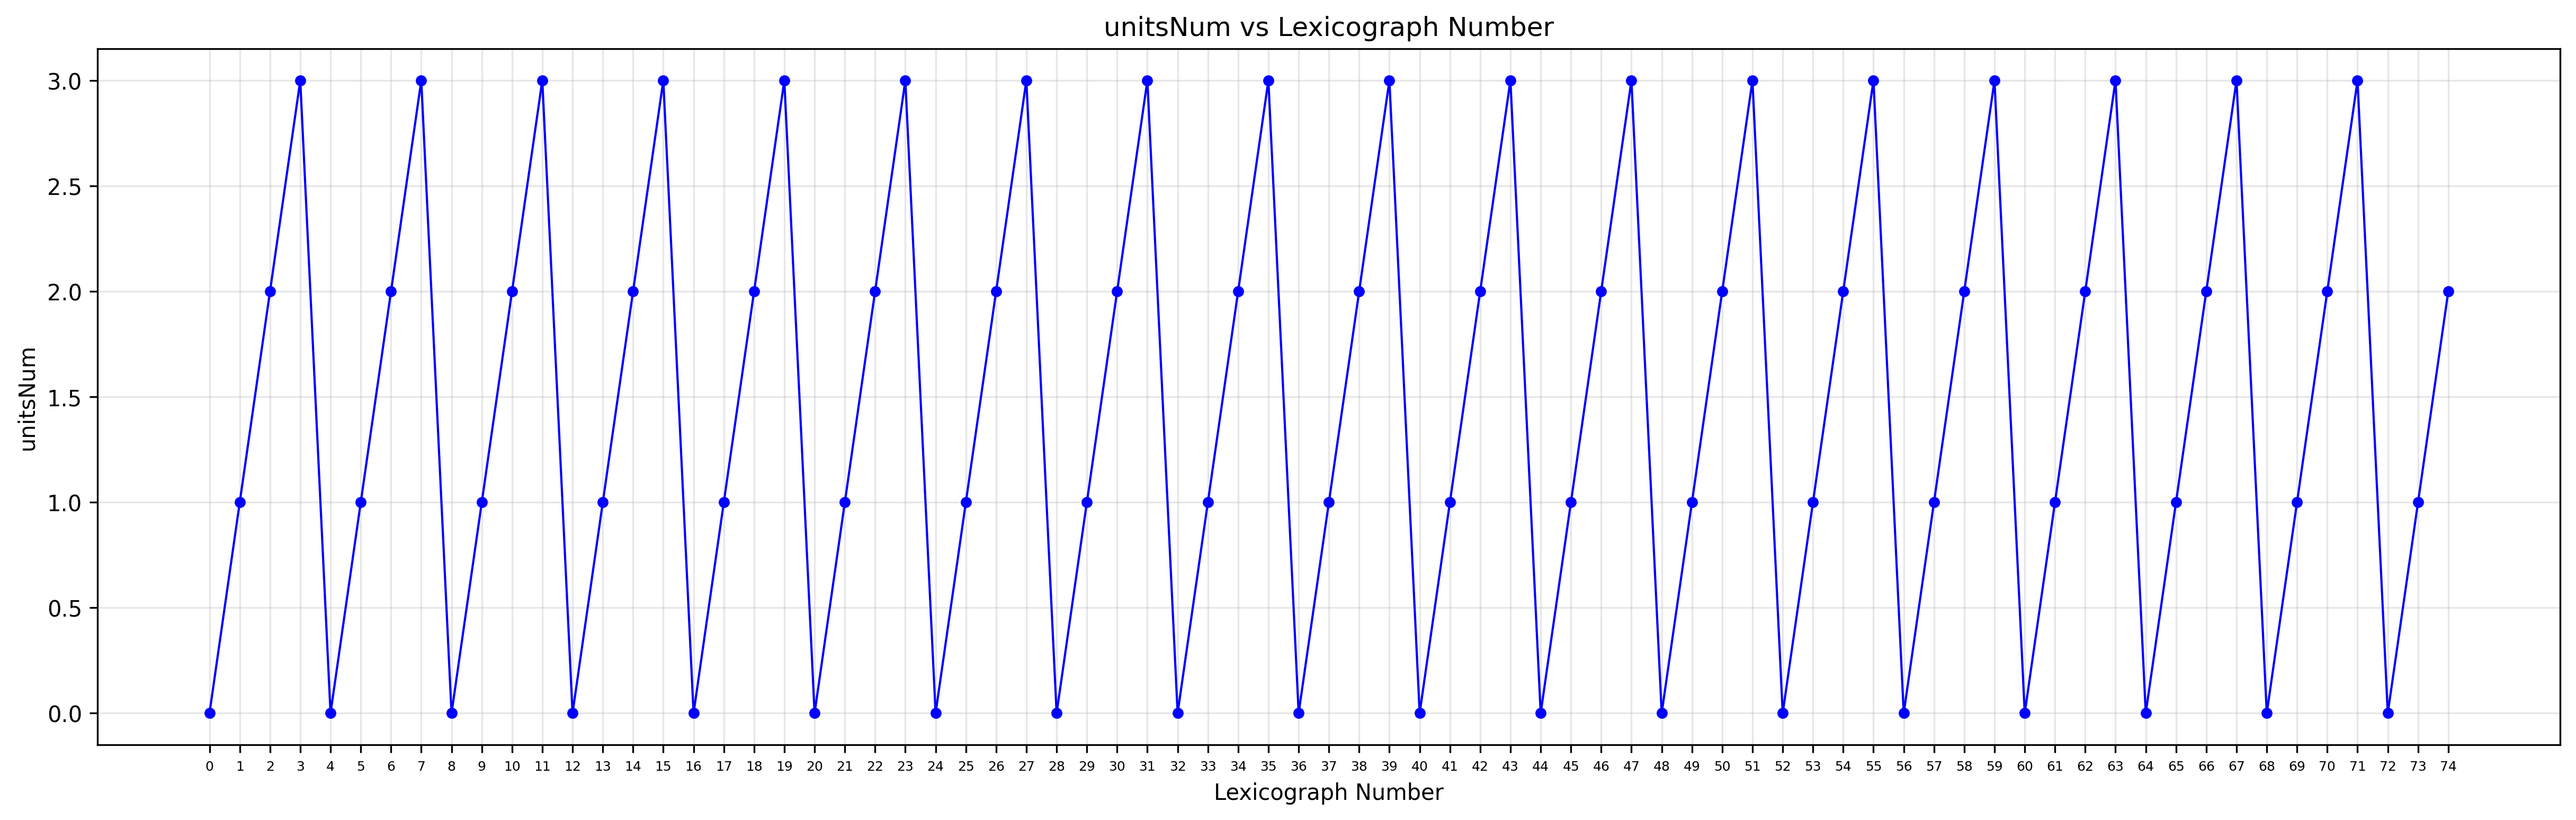
\includegraphics[width=\textwidth]{7-generated-benchmarking/aggregated/unitsNum_plot.png}
    \caption{Units number progression}\label{fig:unitsnum-progression}
  \end{minipage}
  \hfill
  \begin{minipage}{0.8\textwidth}
    \centering
    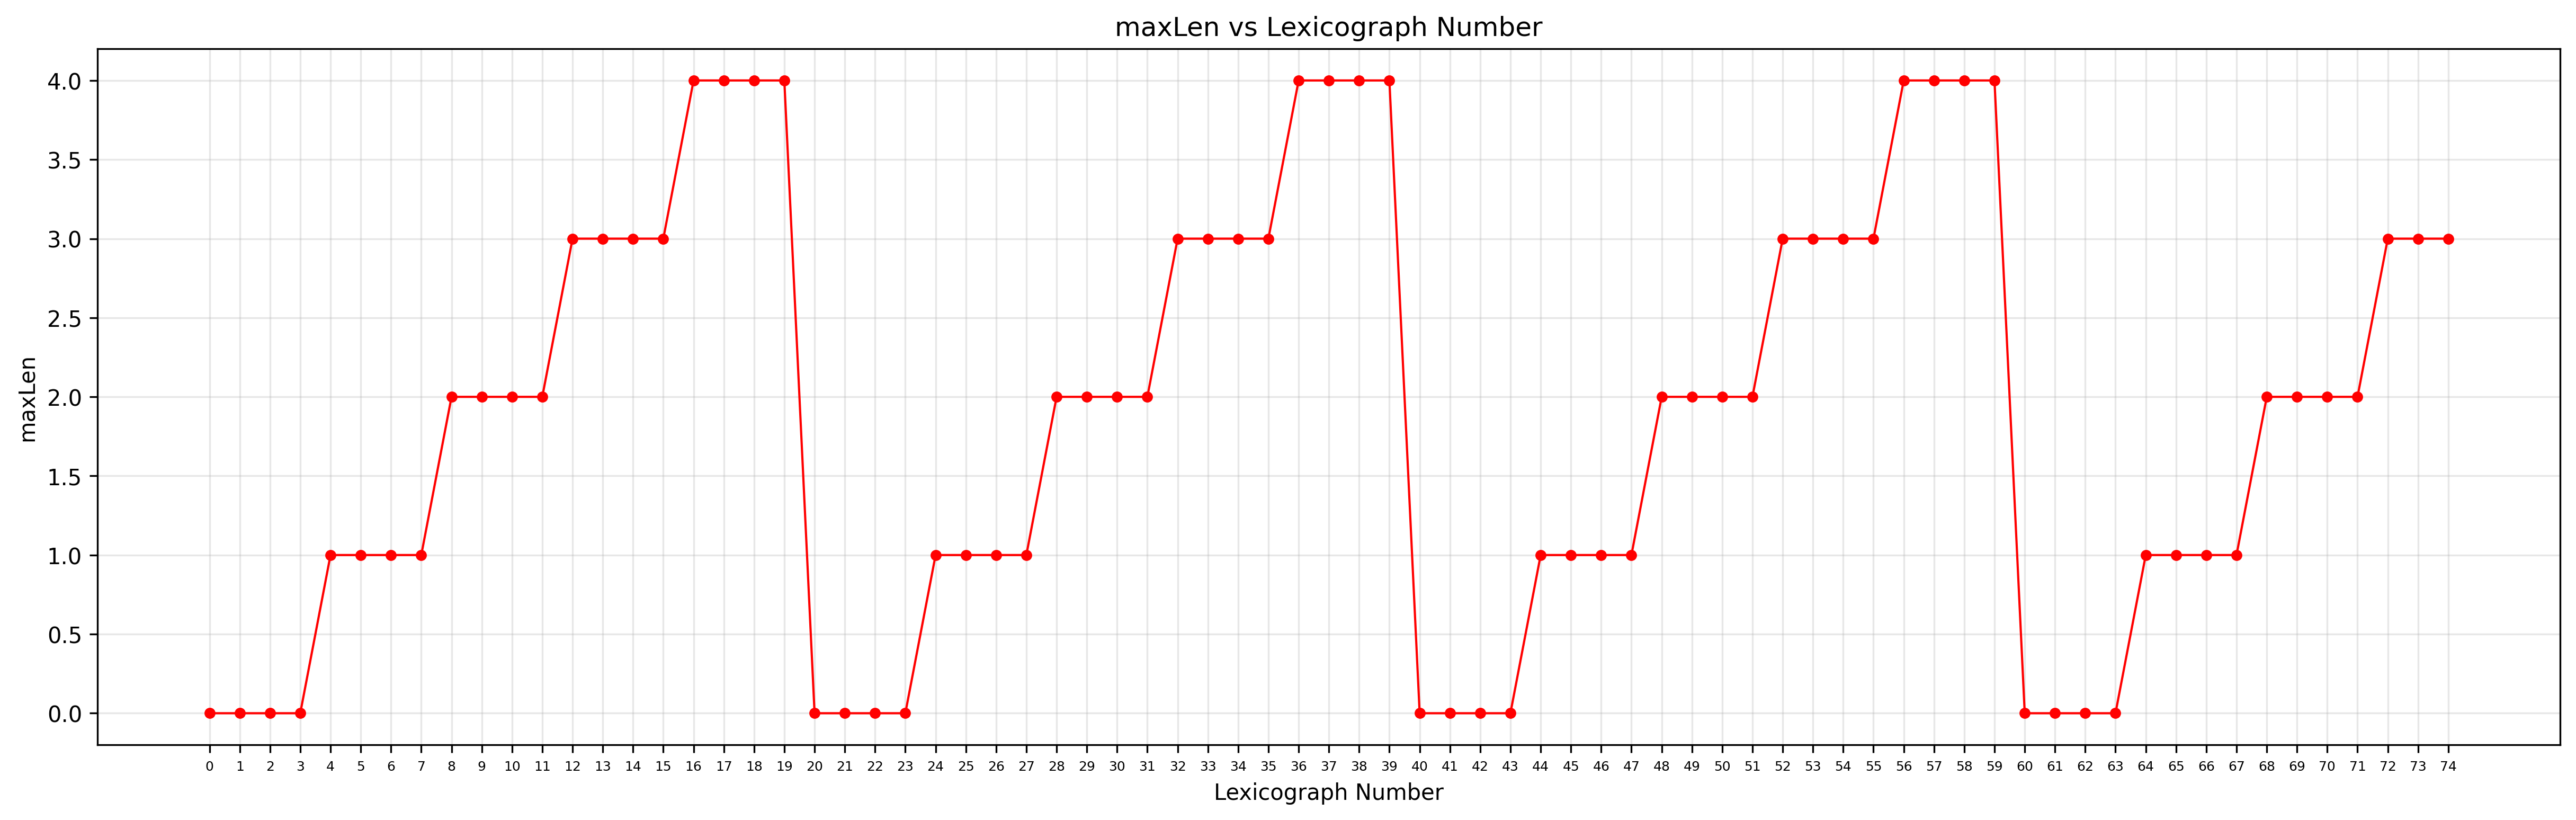
\includegraphics[width=\textwidth]{7-generated-benchmarking/aggregated/maxLenIdx_plot.png}
    \caption{Maximal length progression}\label{fig:maxlen-progression}
  \end{minipage}
\end{figure}
\begin{figure}[H]
  \centering
  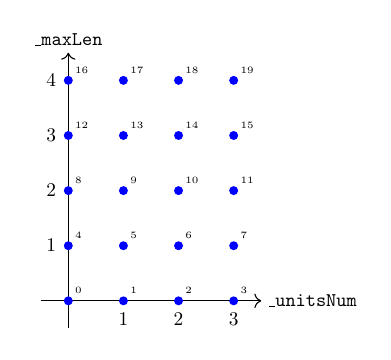
\begin{tikzpicture}[scale=0.7,transform shape]
    % Assi
    \draw[->] (-0.5,0) -- (3.5,0) node[right] {\texttt{\_unitsNum}};
    \draw[->] (0,-0.5) -- (0,4.5) node[above] {\texttt{\_maxLen}};

    % Puntini e label
    \foreach \x in {0,...,3} {
      \foreach \y in {0,...,4} {
        \filldraw[blue] (\x,\y) circle (2pt);
        \node[anchor=south west, font=\tiny] at (\x,\y) {\pgfmathtruncatemacro{\result}{\x+\y*4}\result};
      }
    }

    % Tick labels per x
    \foreach \x in {1,...,3} {
      \node[below] at (\x,-0.1) {\x};
    }

    % Tick labels per y
    \foreach \y in {1,...,4} {
      \node[left] at (-0.1,\y) {\y};
    }
  \end{tikzpicture}
  \caption{Encoding of \code{_maxLen} and \code{_unitsNum} in the lexicographic ordering.}\label{fig:maxlen-unitsnum-encoding}
\end{figure}
This is probably due to the fact that having a high maximum length allows for more complex formulae, while having a low number of units means that there are fewer opportunities for contradictions to be generated, leading to longer resolution times.
A good analogy can be made with natural language texts: a text composed of a few long sentences is generally harder to understand than a text composed of many short sentences, as the latter provides more opportunities for clarification and resolution of ambiguities.
To further investigate this phenomenon, we provided an additional chart that aggregates the results based on \code{_maxLen} and \code{_unitsNum} alone, averaging over all values of \code{_predNum} and \code{_maxArity}.

\begin{figure}[H]
  \centering
  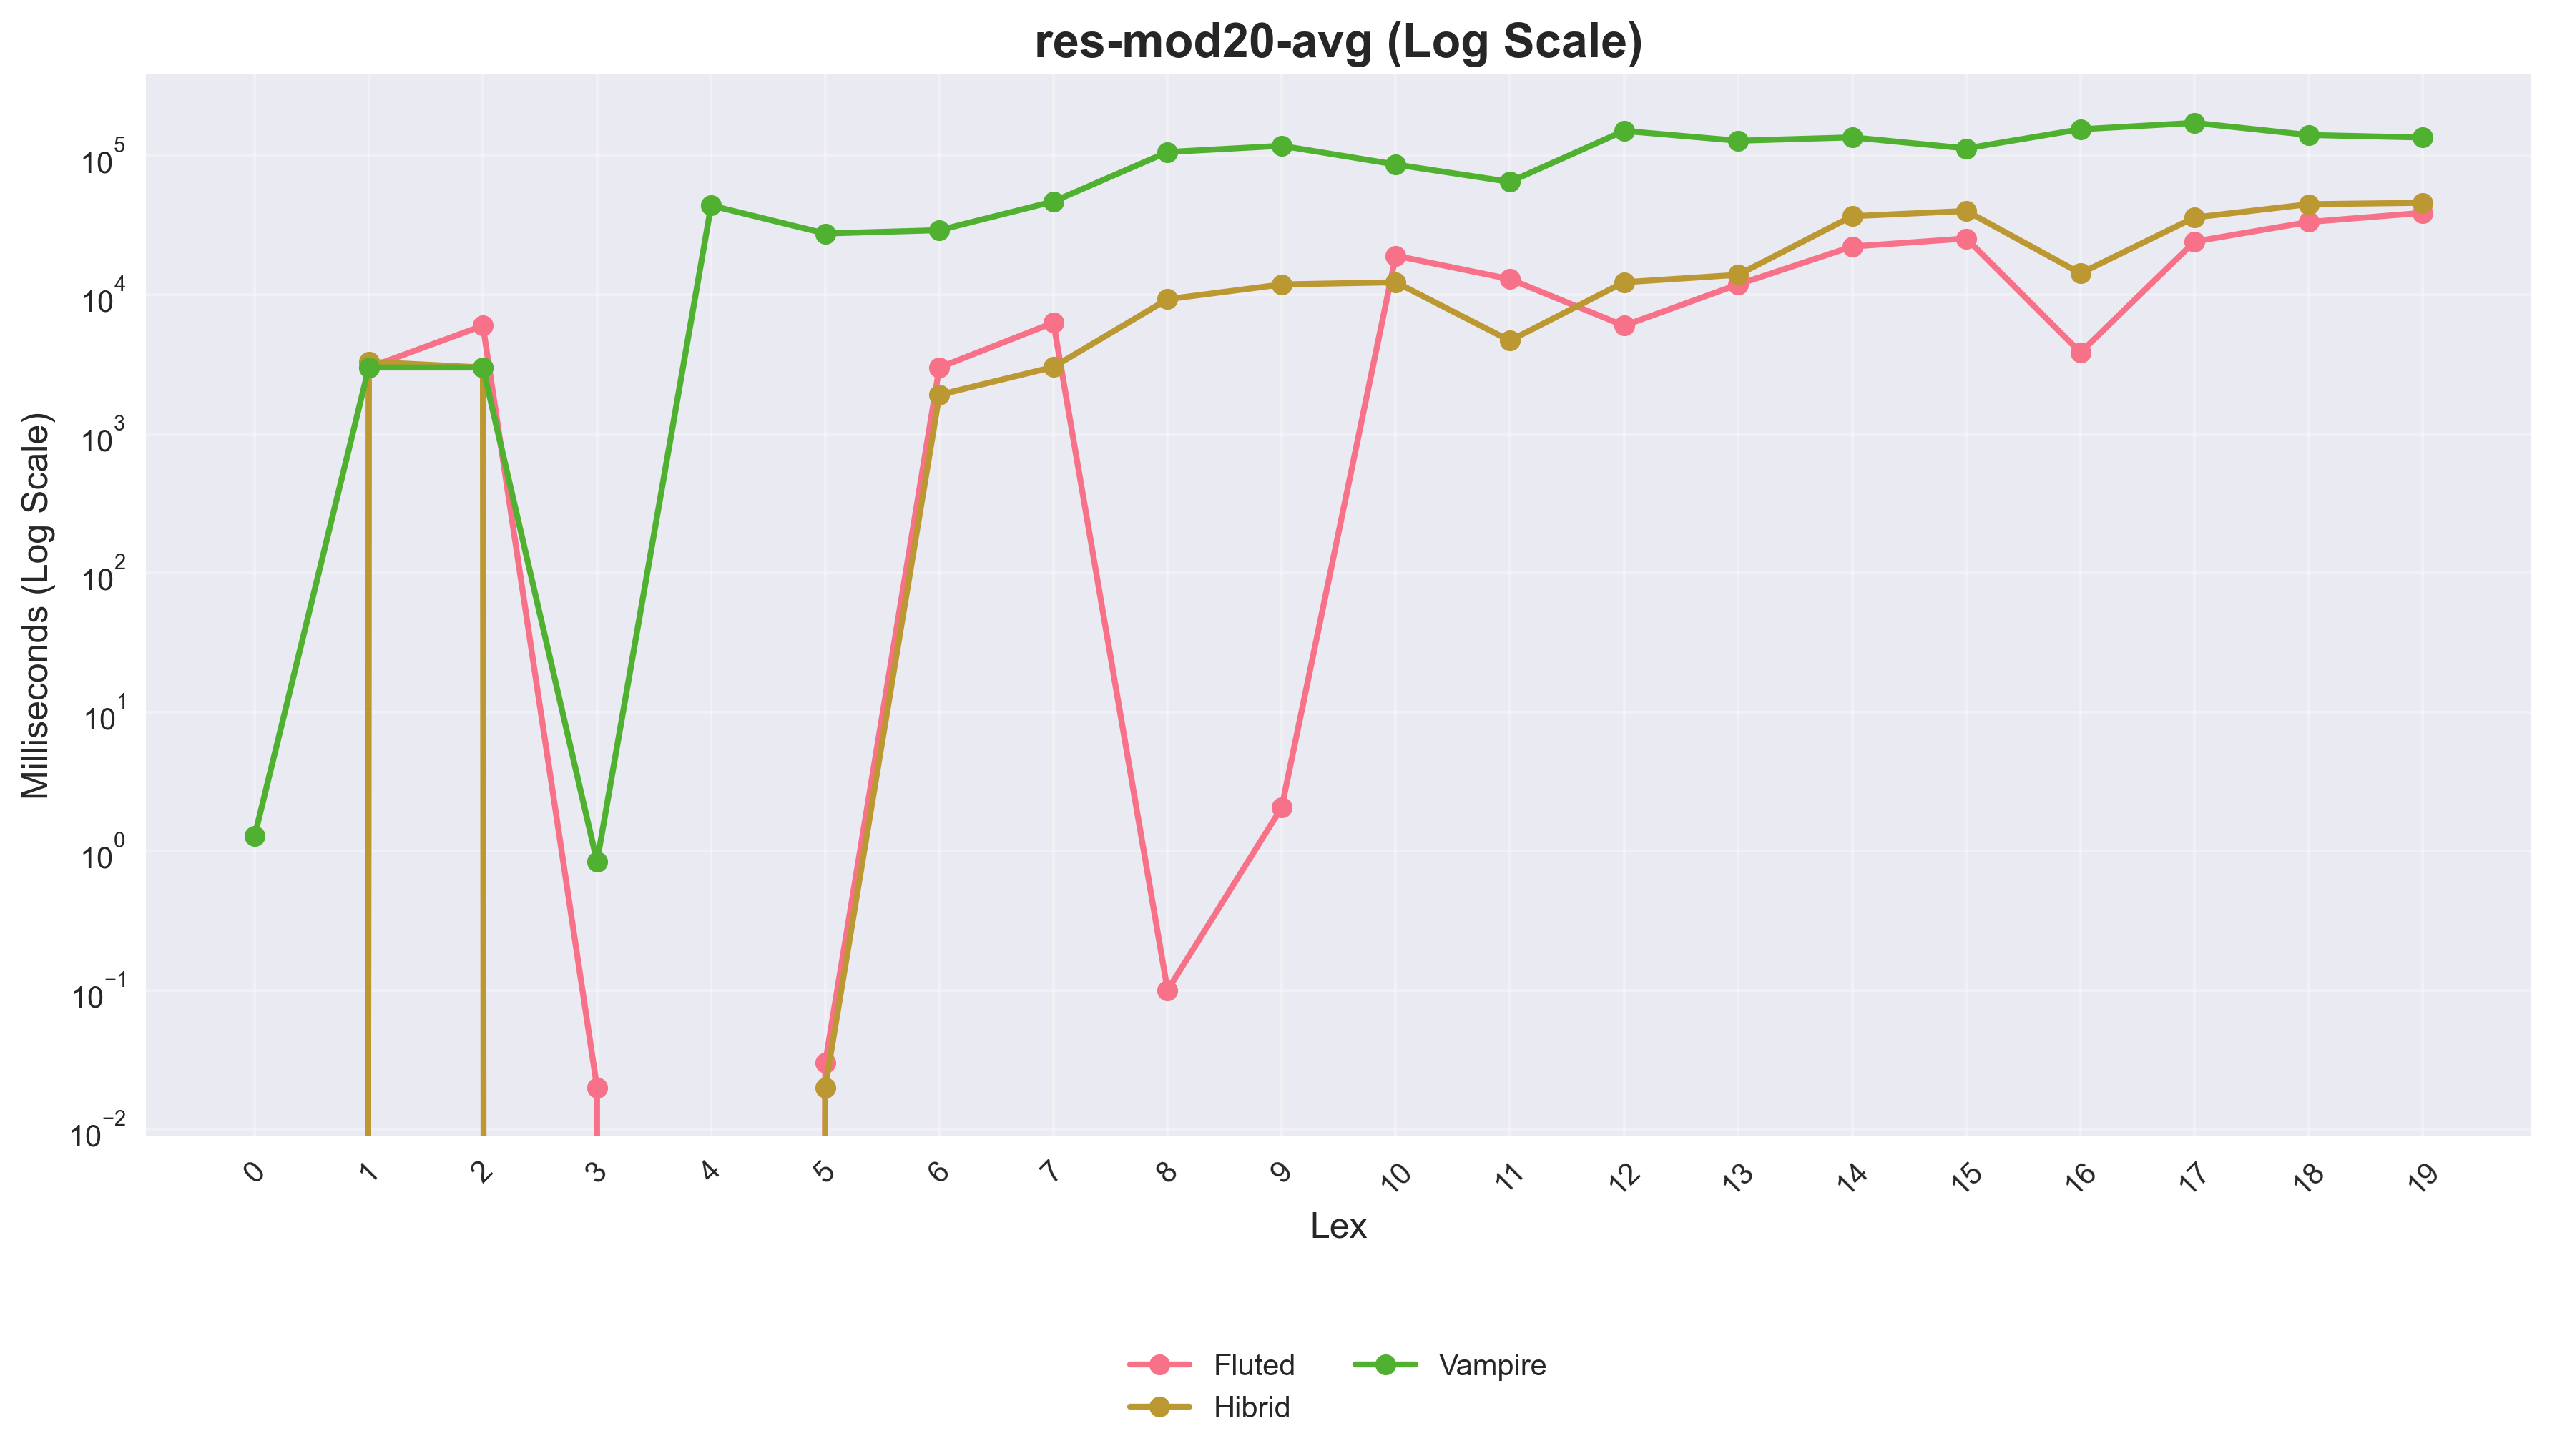
\includegraphics[width=0.8\textwidth]{7-generated-benchmarking/aggregated/res-mod20-avg_linee_log.png}
\end{figure}
\begin{figure}[H]
  \centering
  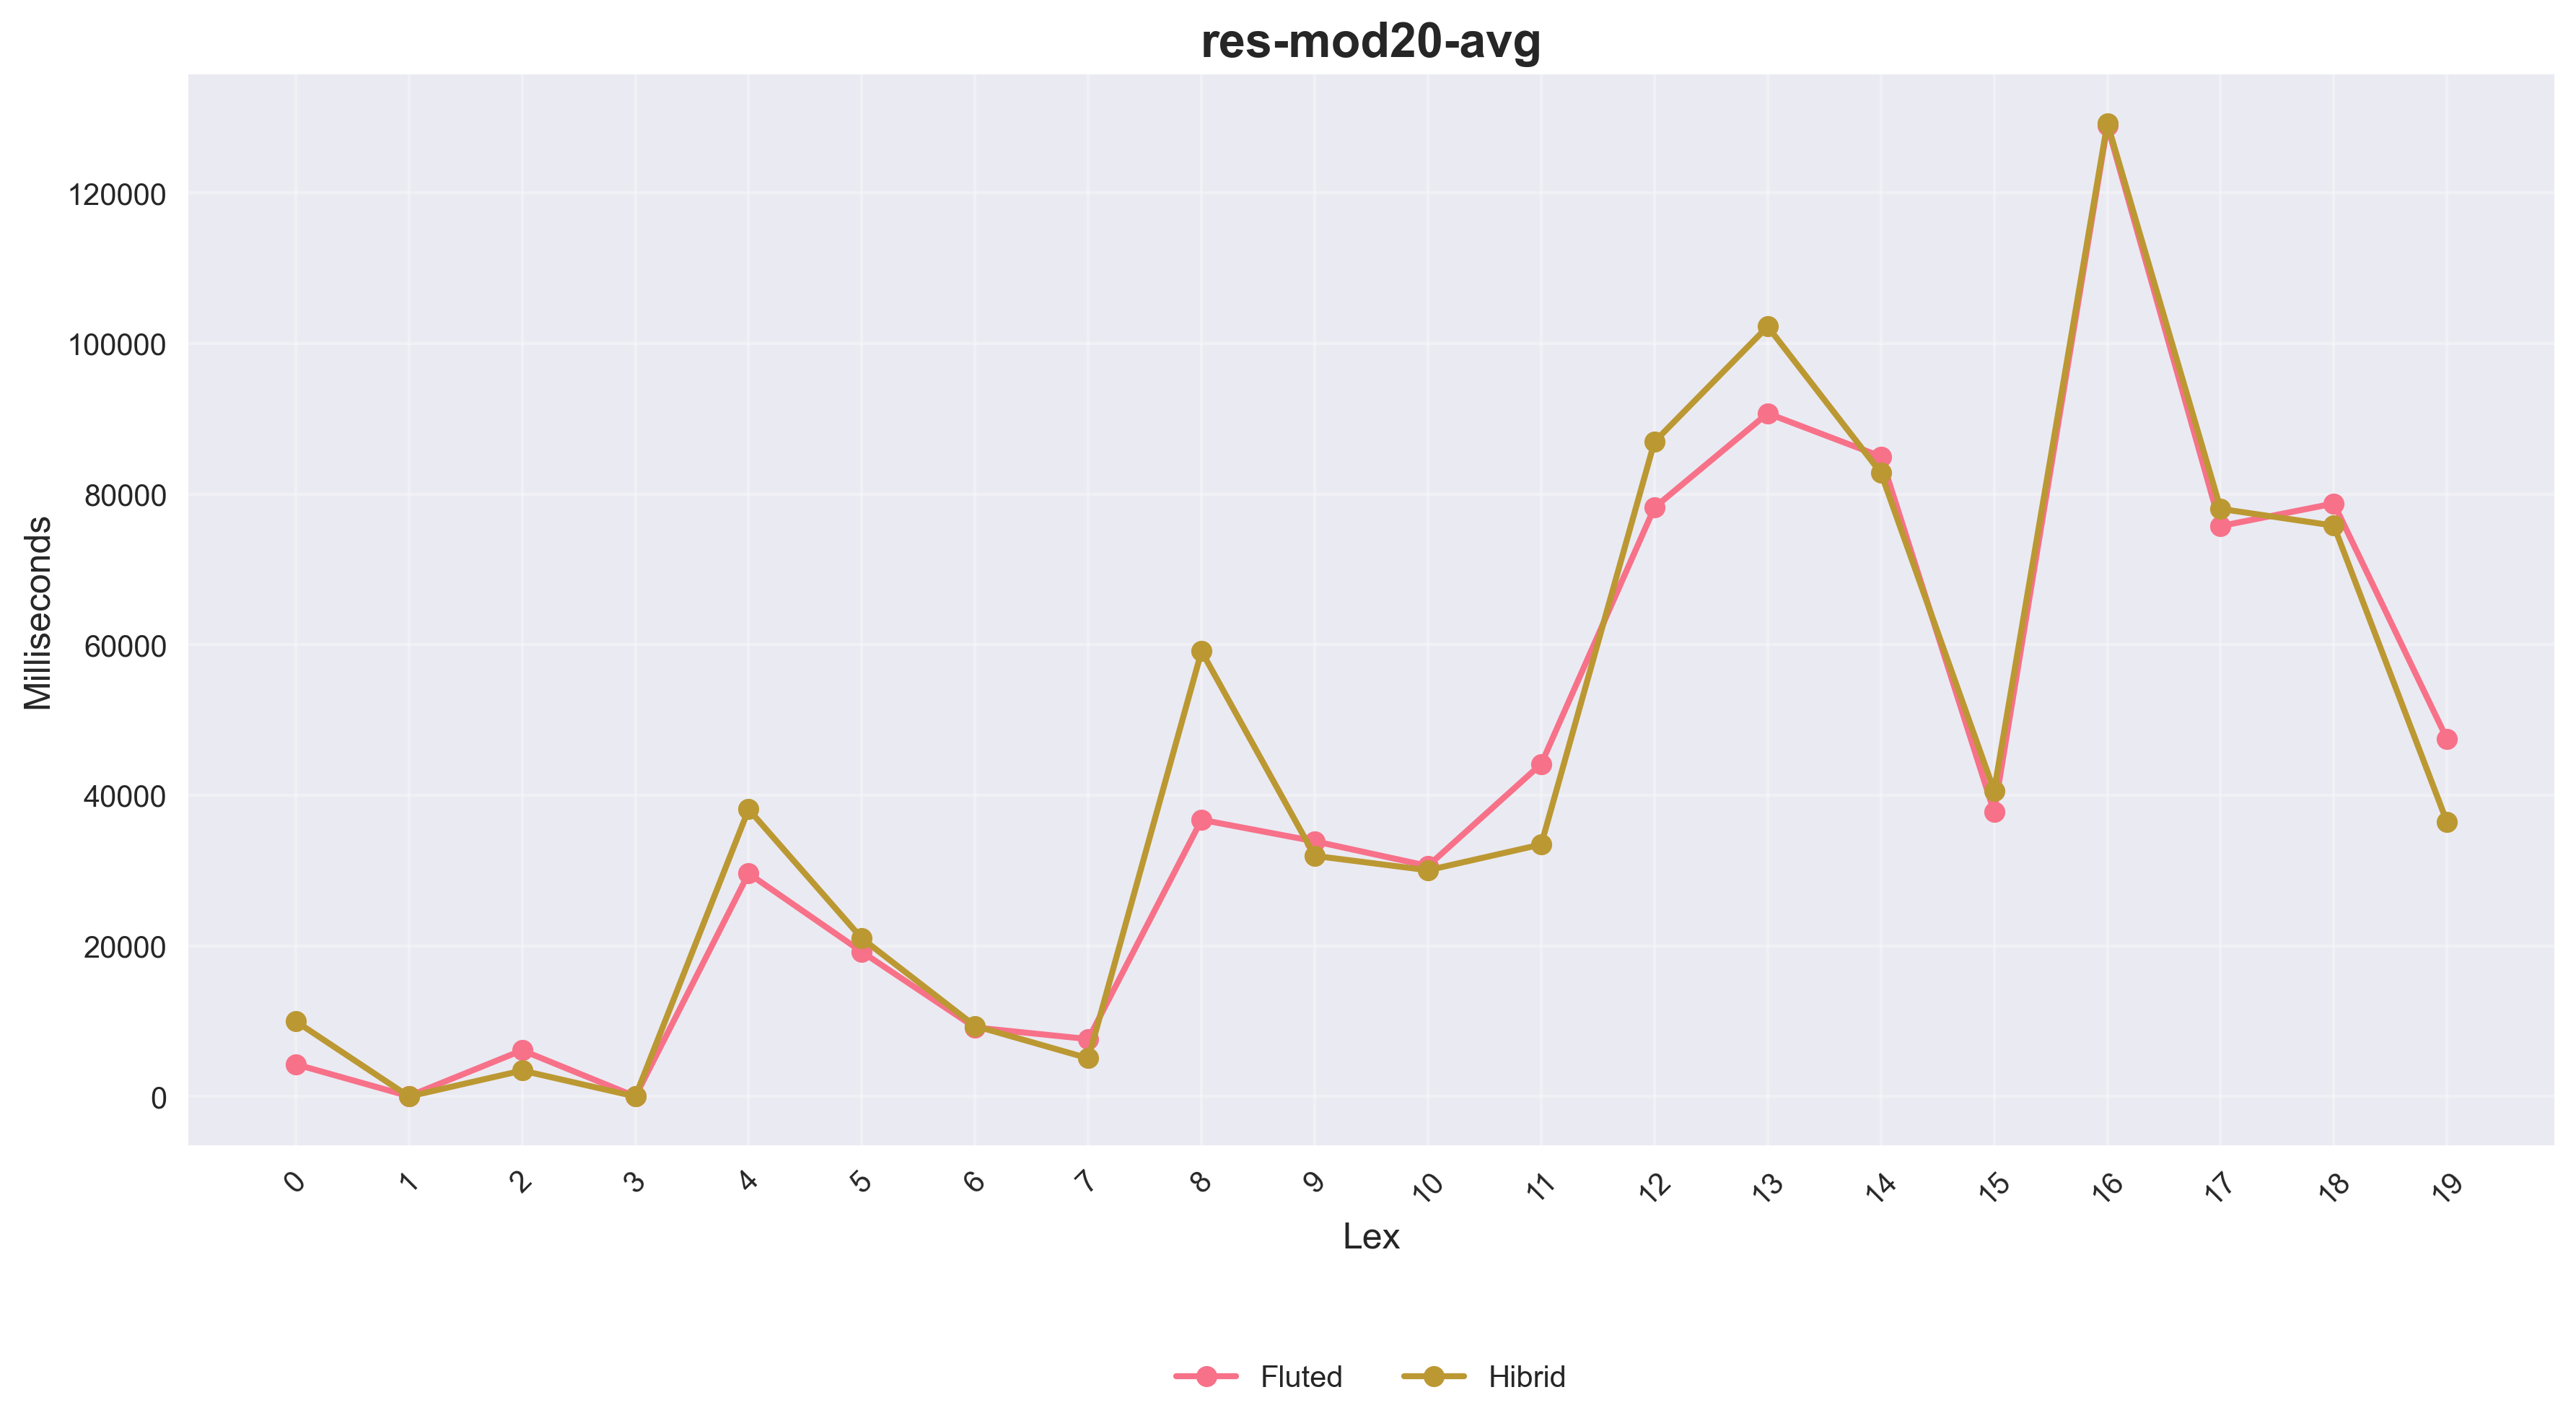
\includegraphics[width=0.8\textwidth]{7-generated-benchmarking/aggregated/res-mod20-avg_linee_normal.png}
  \caption{Aggregated results for generated problems with respect to \code{_maxLen} and \code{_unitsNum}.}\label{fig:agg-maxlen-unitsnum}
\end{figure}
The aggregated versions of the charts with respect to the \code{_predNum} parameter only, with the variable fixed, are provided in Appendix~\ref{app:charts-by-maxlen-unitsnum}.

After this interesting finding, we moved on to analyse the impact of the number of variables on the performance.
To do so, we aggregated the results based on \code{_maxArity} alone, initially fixing the other three parameters.
What follows are examples of such charts, with the full set available in the repository mentioned above.

\begin{figure}[H]
  \centering
  \begin{minipage}{1\textwidth}
    \centering
    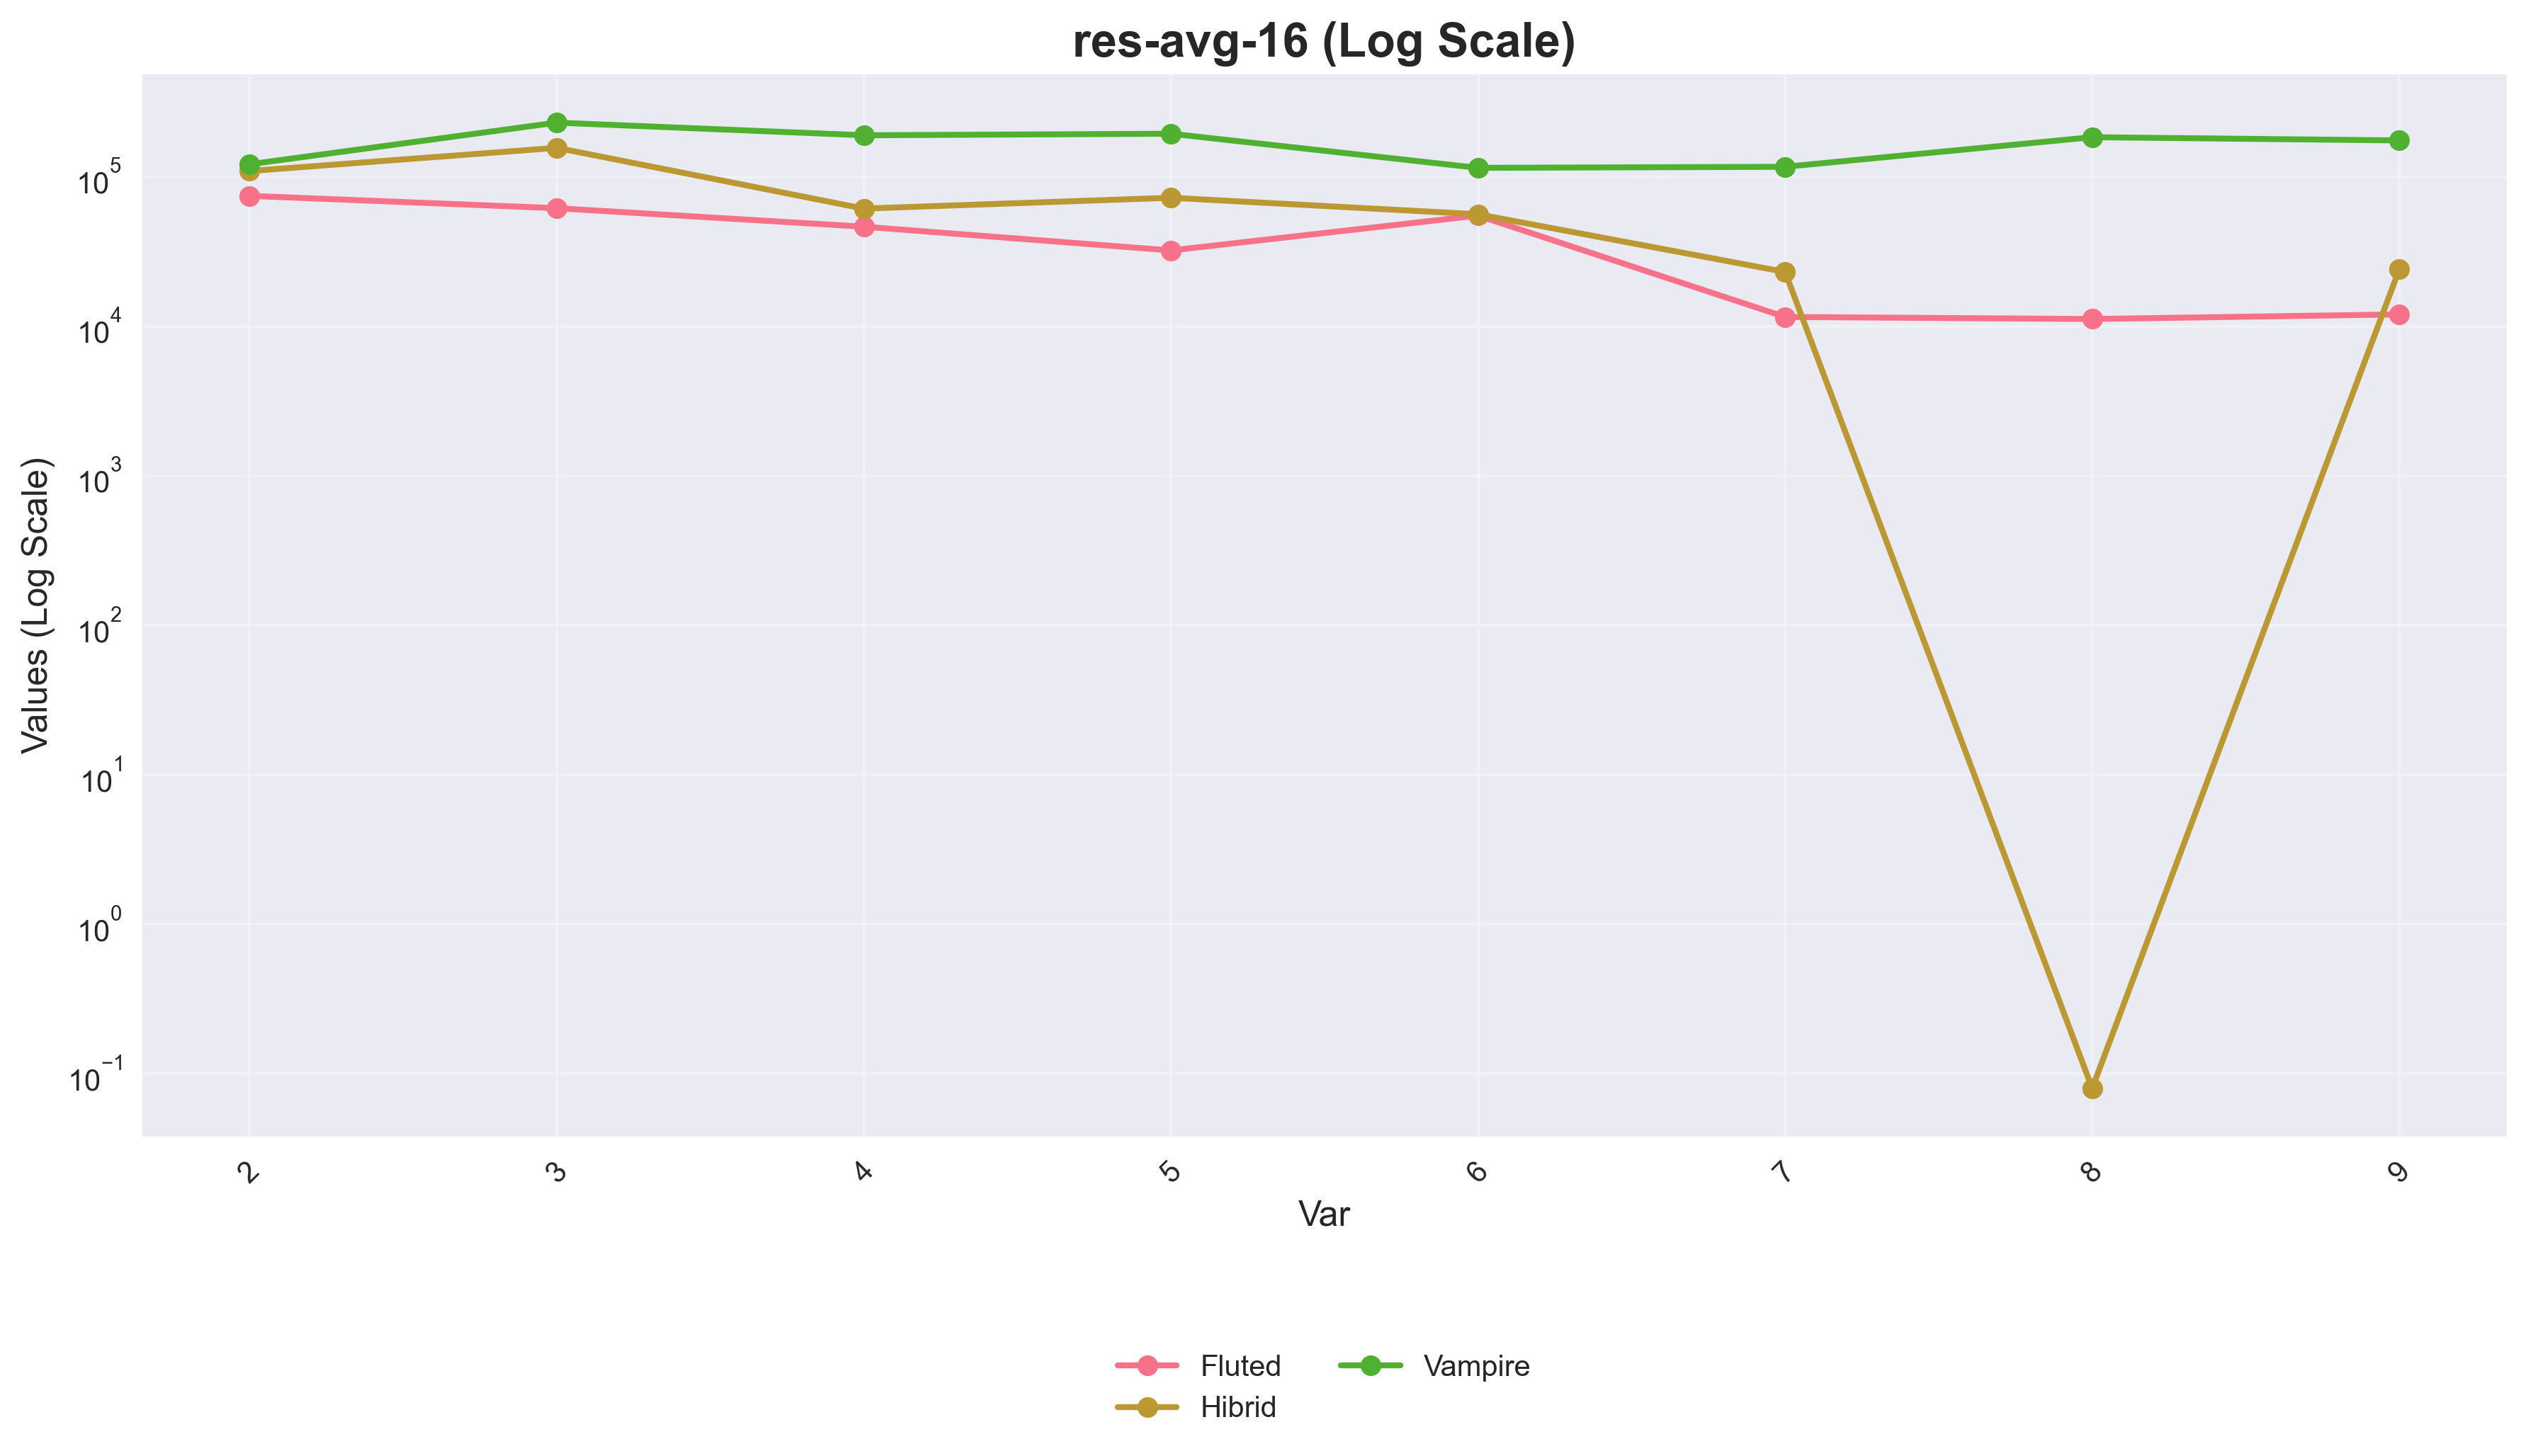
\includegraphics[width=\textwidth]{7-generated-benchmarking/aggregated/res-avg-16_linee_log.png}
  \end{minipage}
  \hfill
  \begin{minipage}{1\textwidth}
    \centering
    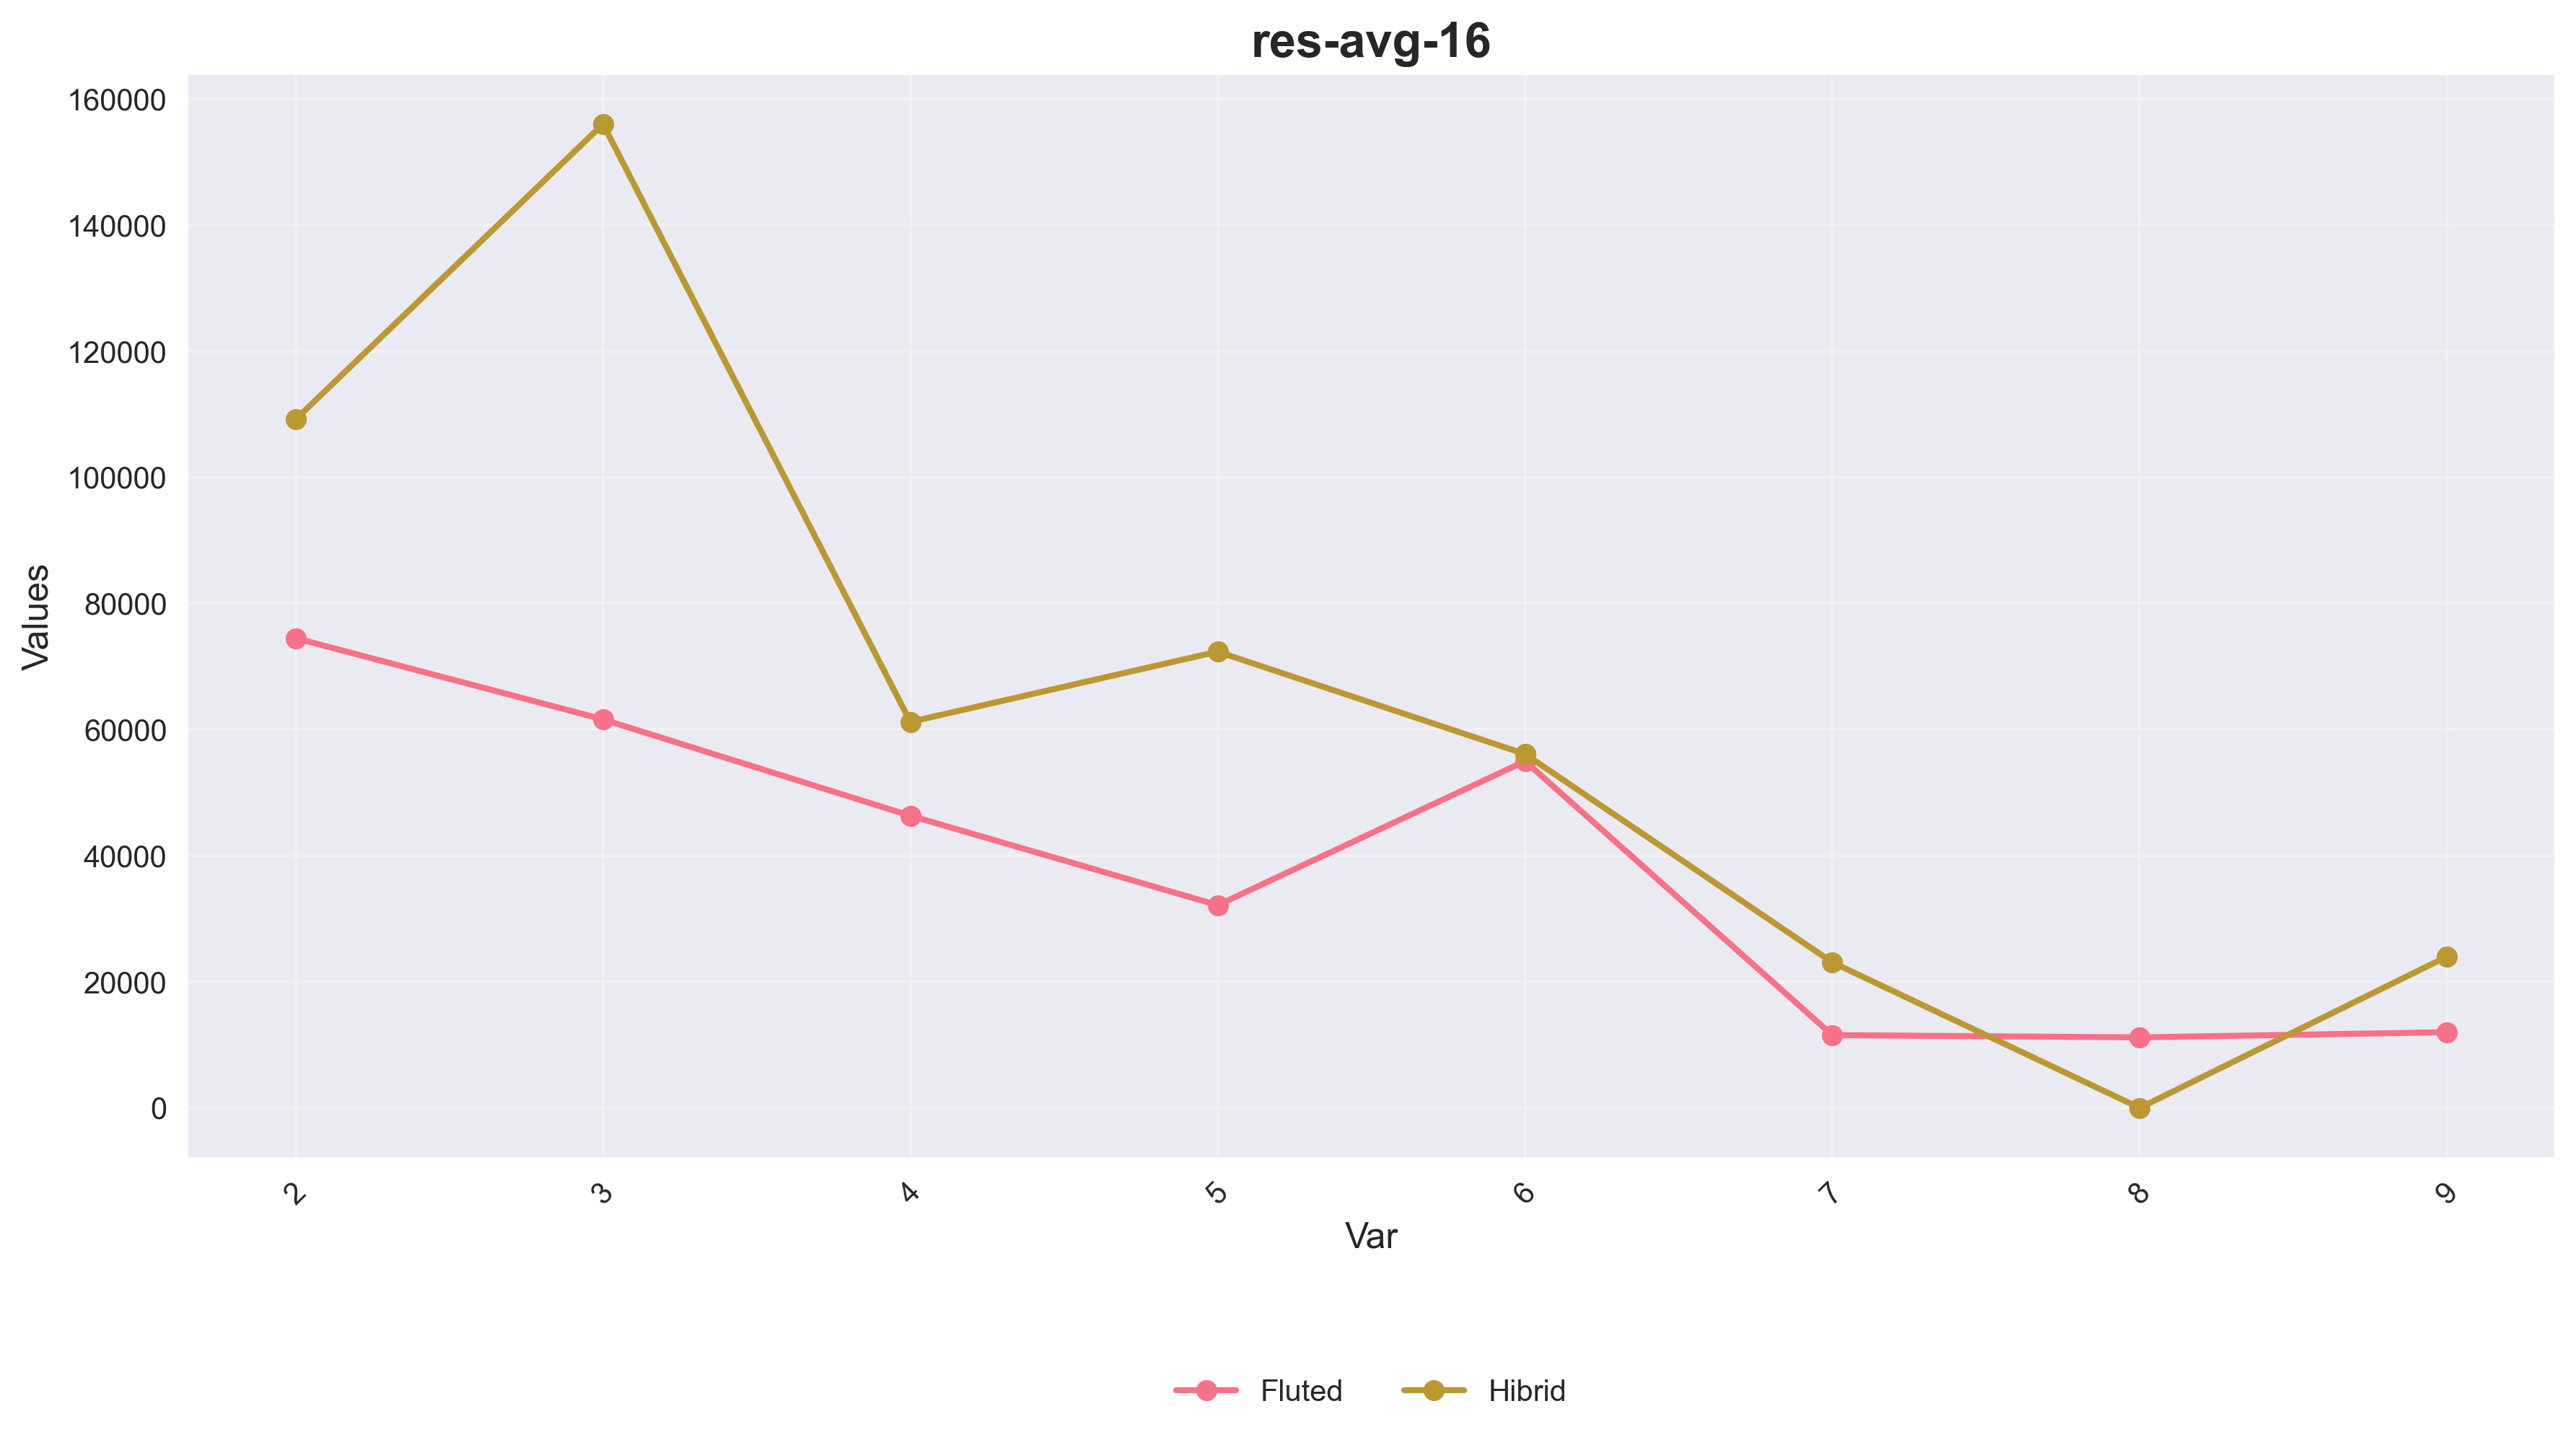
\includegraphics[width=\textwidth]{7-generated-benchmarking/aggregated/res-avg-16_linee_normal.png}
  \end{minipage}
  \caption{Aggregated results for generated problems with lexicographic encoding 16.}\label{fig:agg-le16}
\end{figure}

\begin{figure}[H]
  \centering
  \begin{minipage}{1\textwidth}
    \centering
    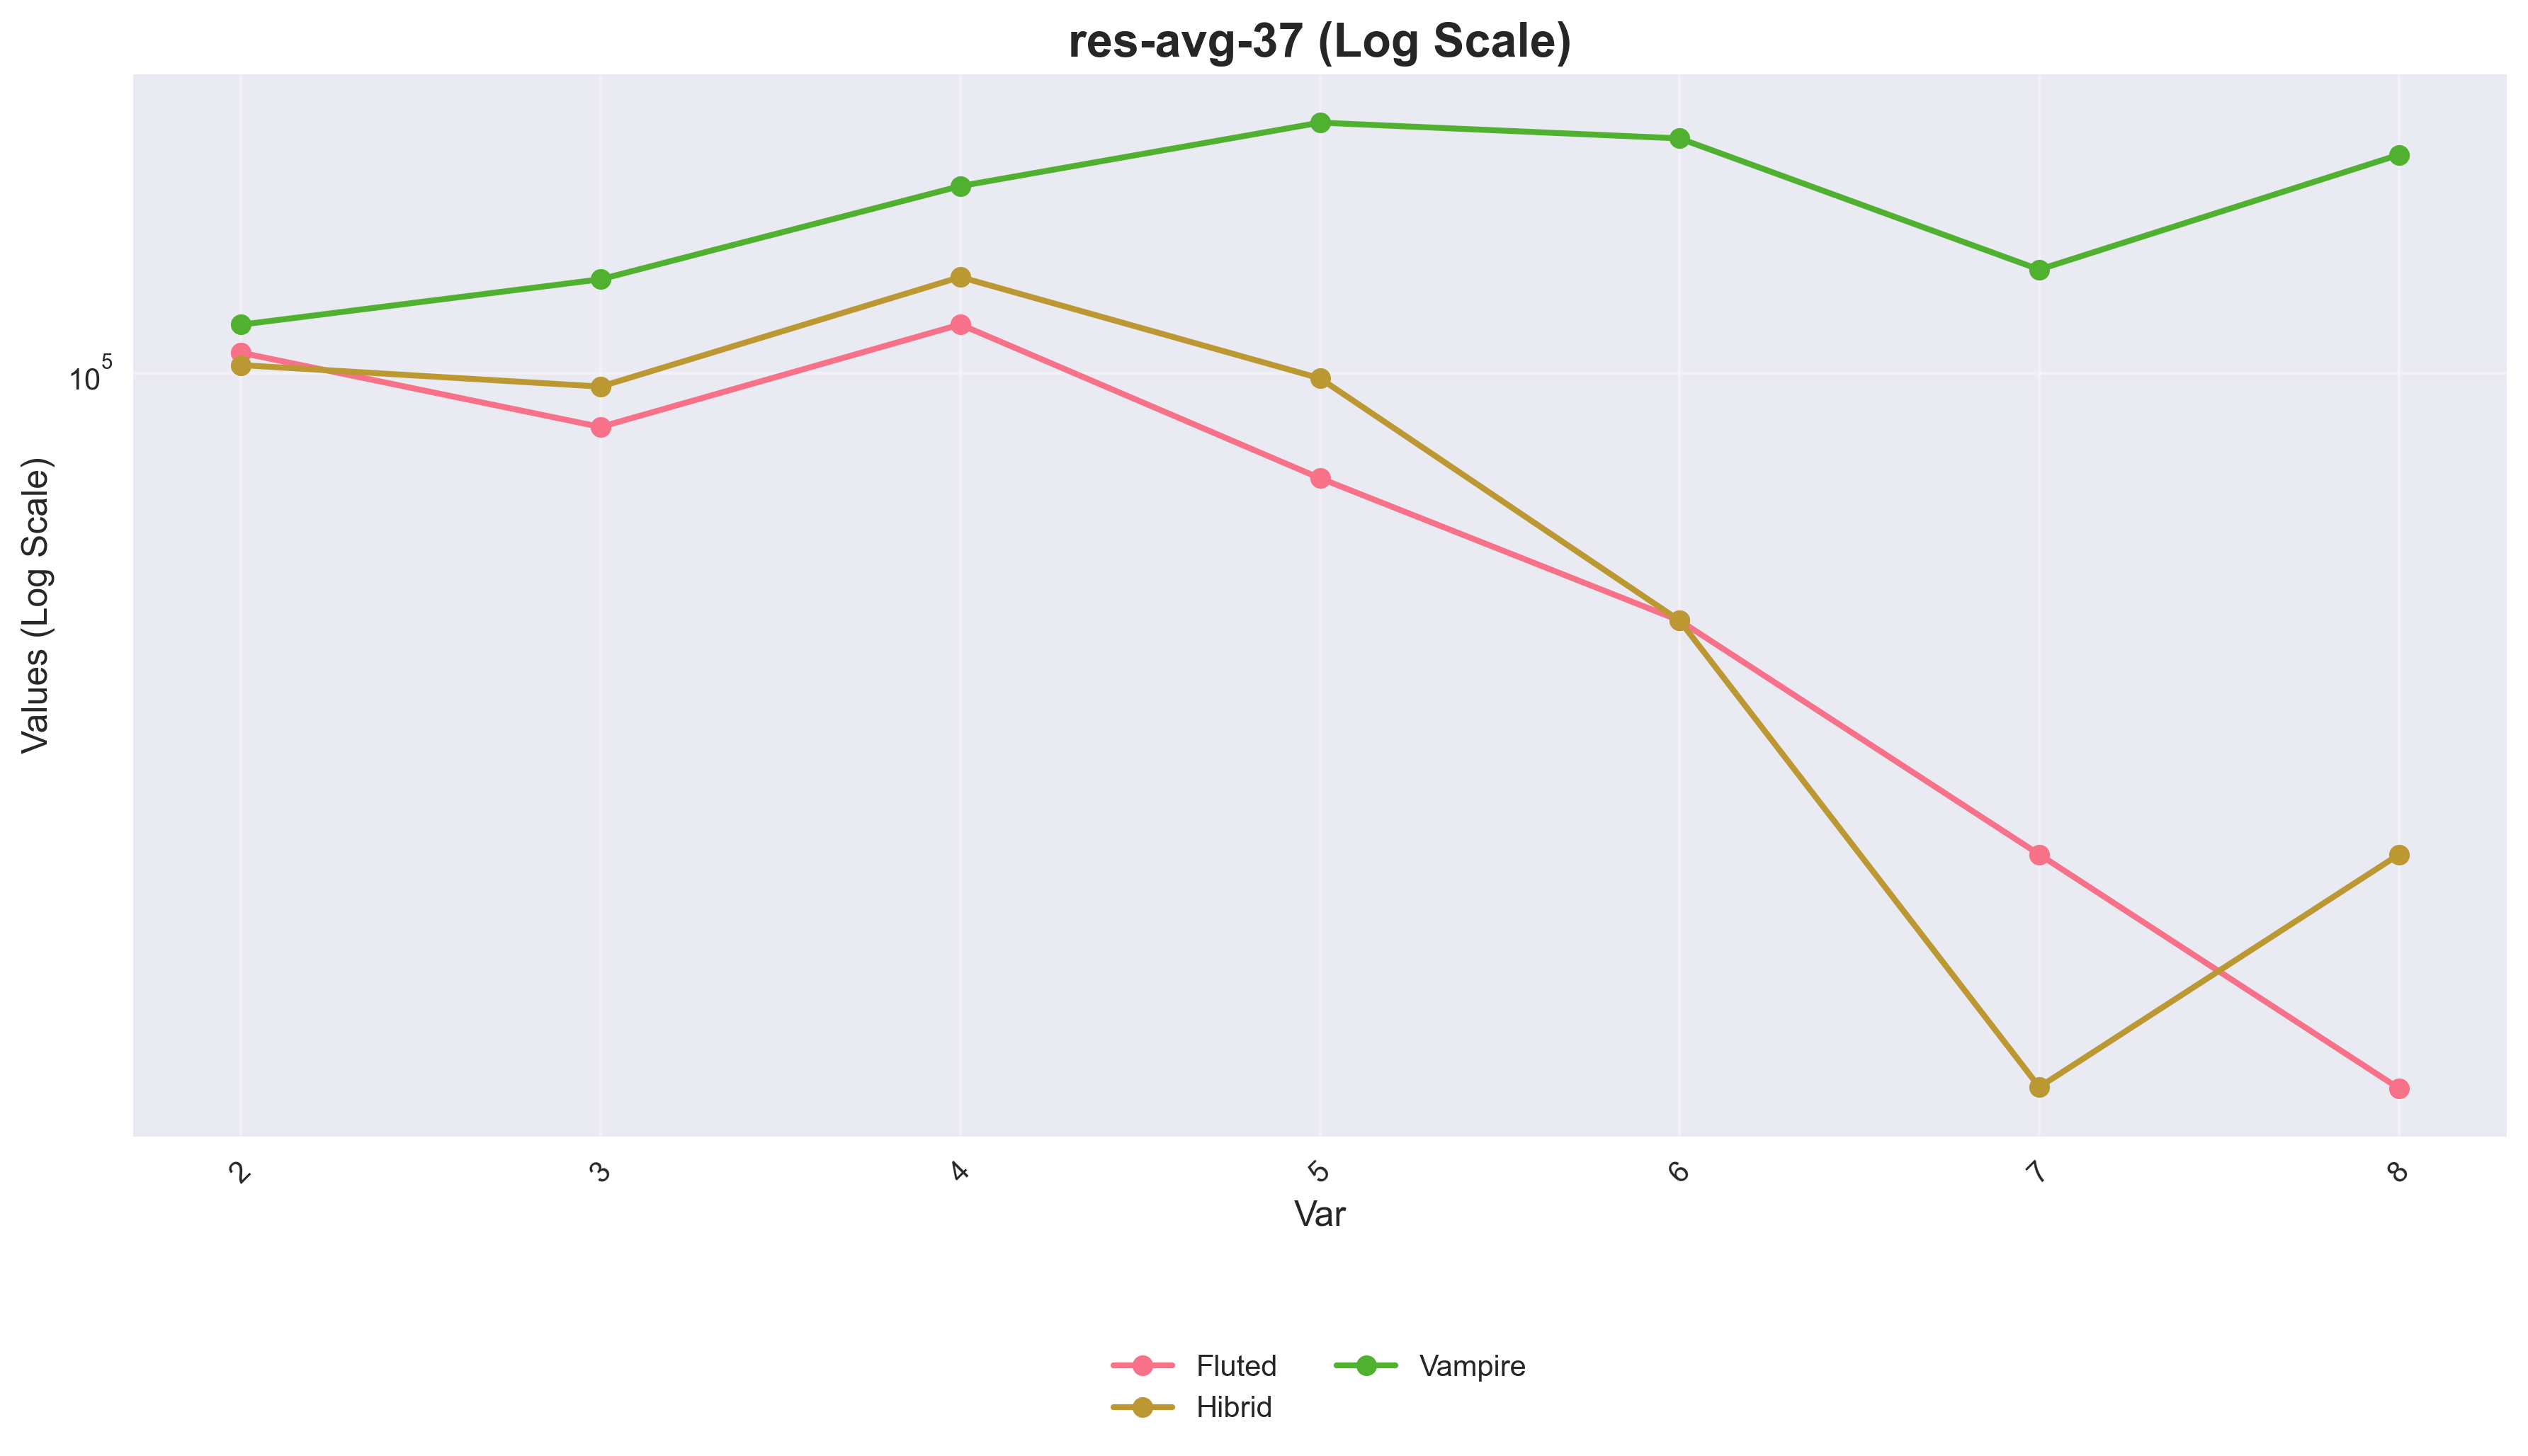
\includegraphics[width=\textwidth]{7-generated-benchmarking/aggregated/res-avg-37_linee_log.png}
  \end{minipage}
  \hfill
  \begin{minipage}{1\textwidth}
    \centering
    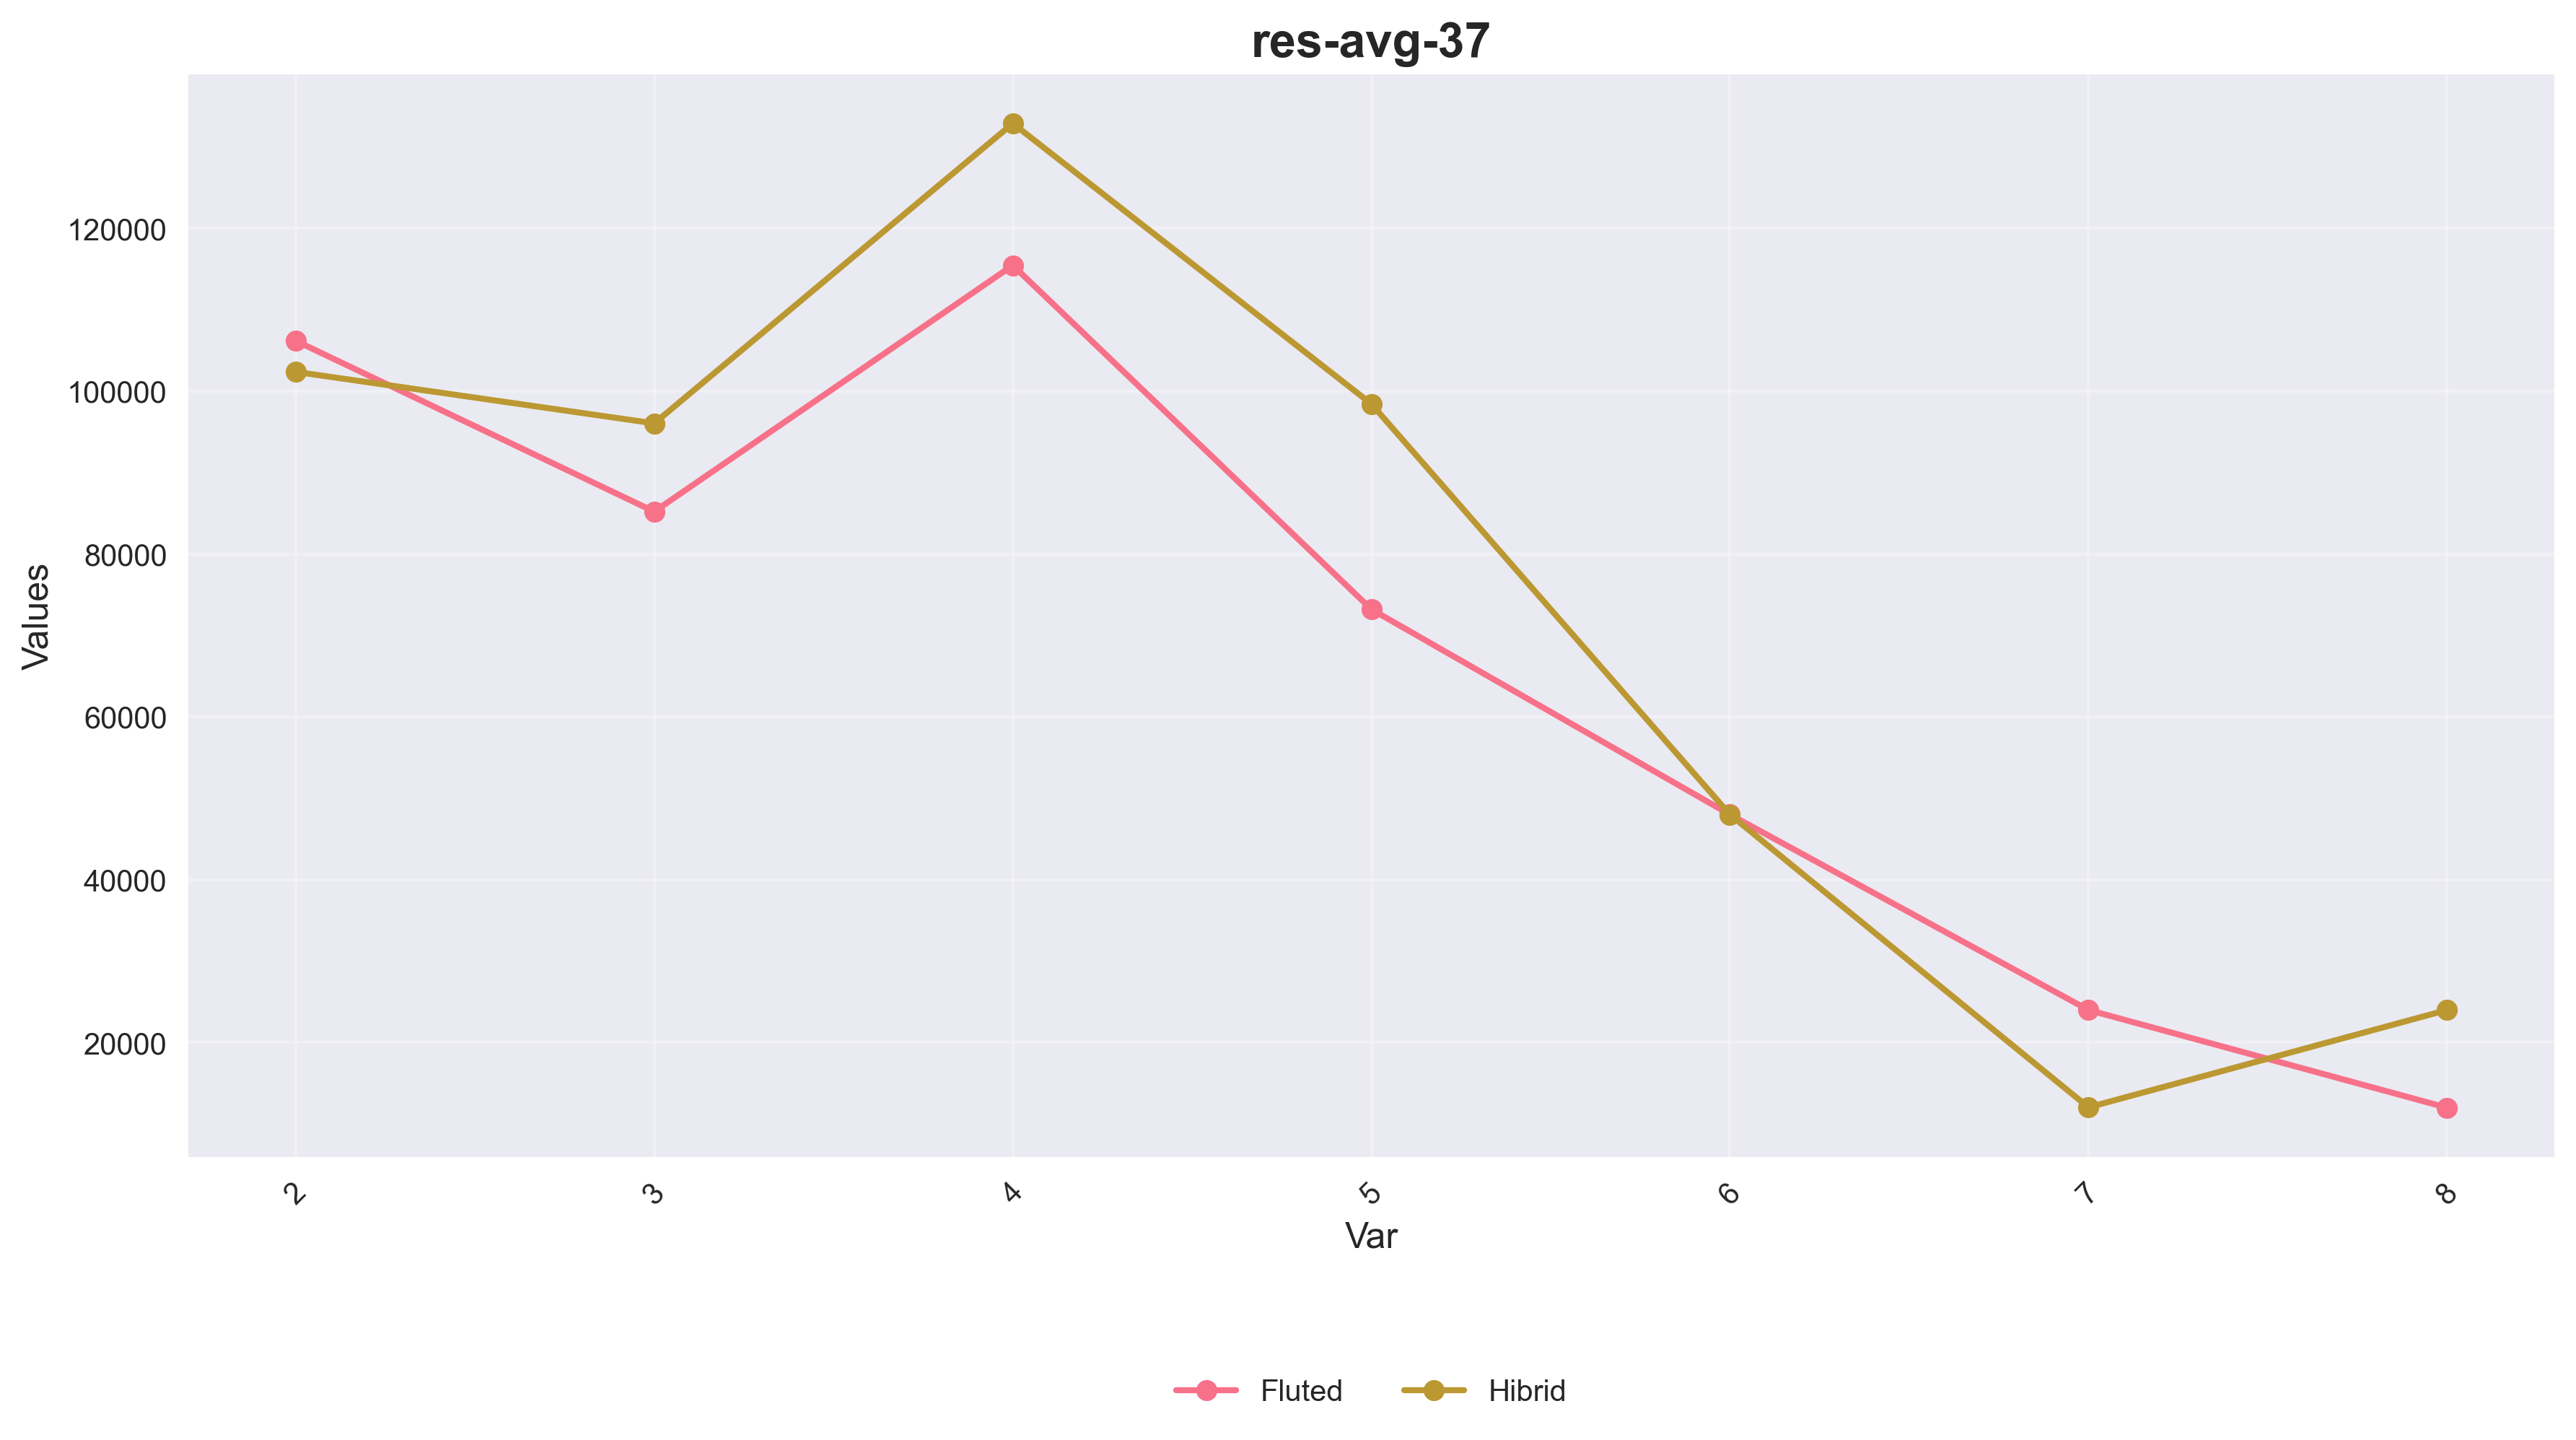
\includegraphics[width=\textwidth]{7-generated-benchmarking/aggregated/res-avg-37_linee_normal.png}
  \end{minipage}
  \caption{Aggregated results for generated problems with lexicographic encoding 37.}\label{fig:agg-le37}
\end{figure}

\begin{figure}[H]
  \centering
  \begin{minipage}{1\textwidth}
    \centering
    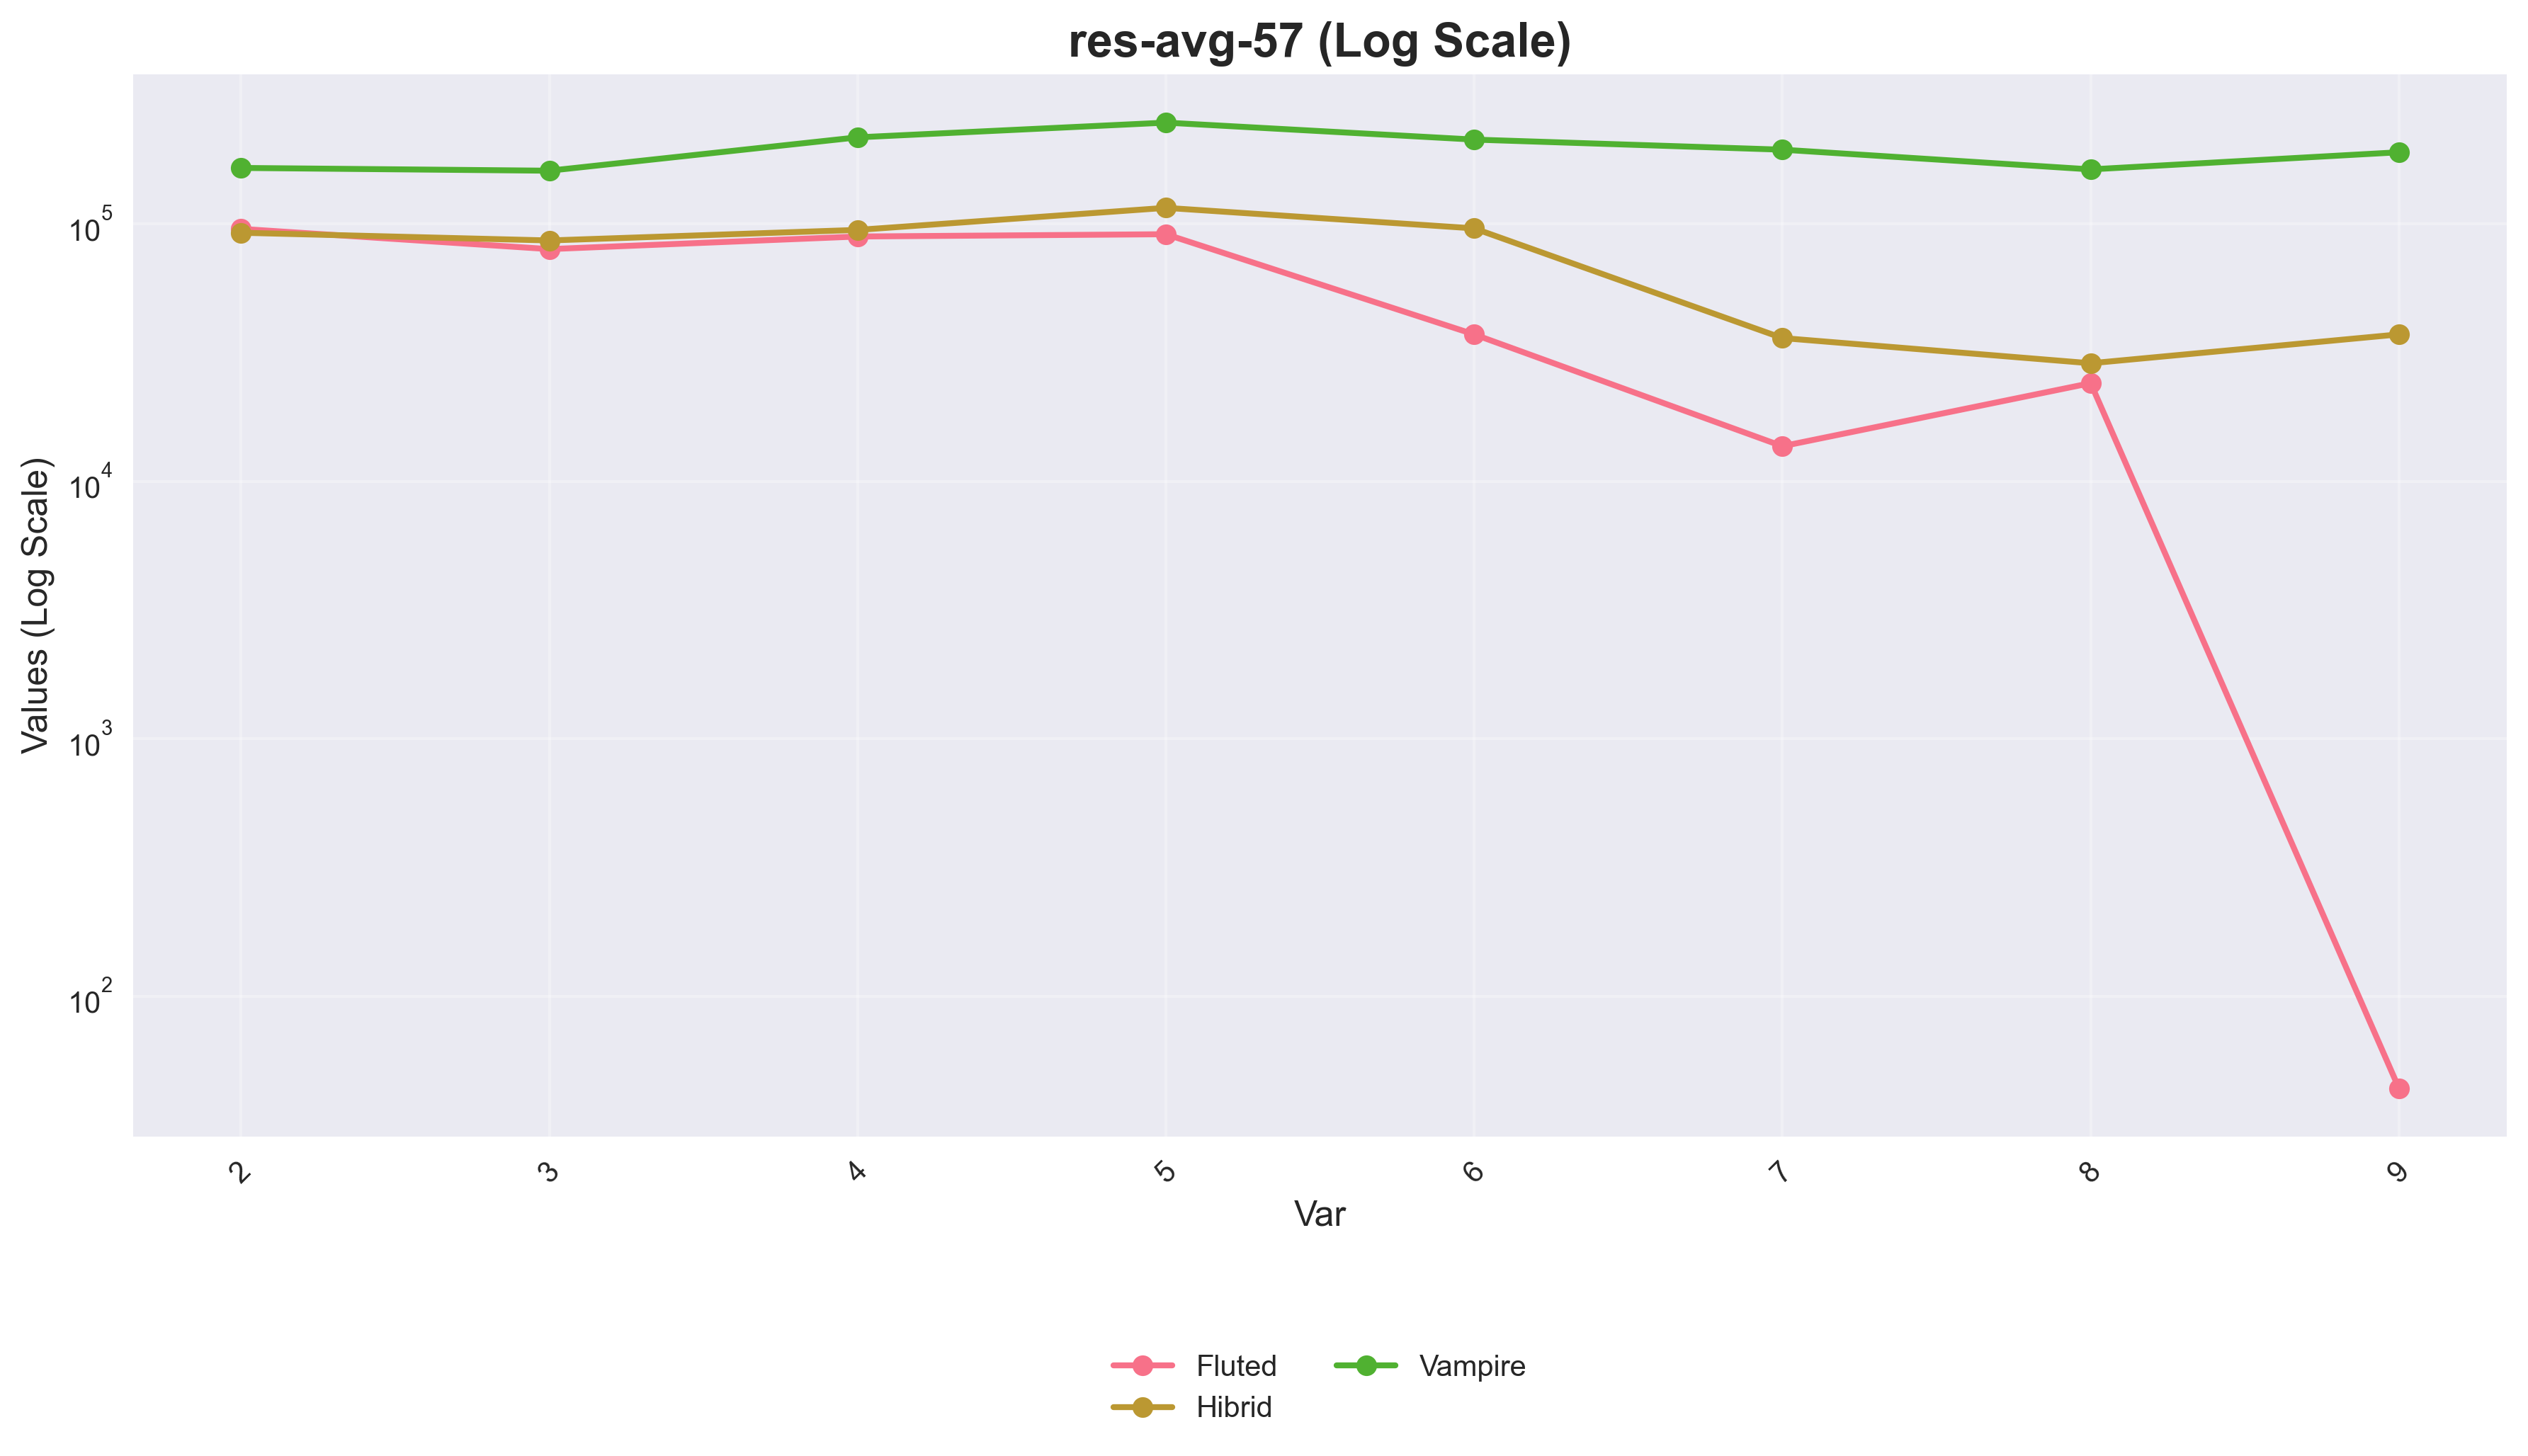
\includegraphics[width=\textwidth]{7-generated-benchmarking/aggregated/res-avg-57_linee_log.png}
  \end{minipage}
  \hfill
  \begin{minipage}{1\textwidth}
    \centering
    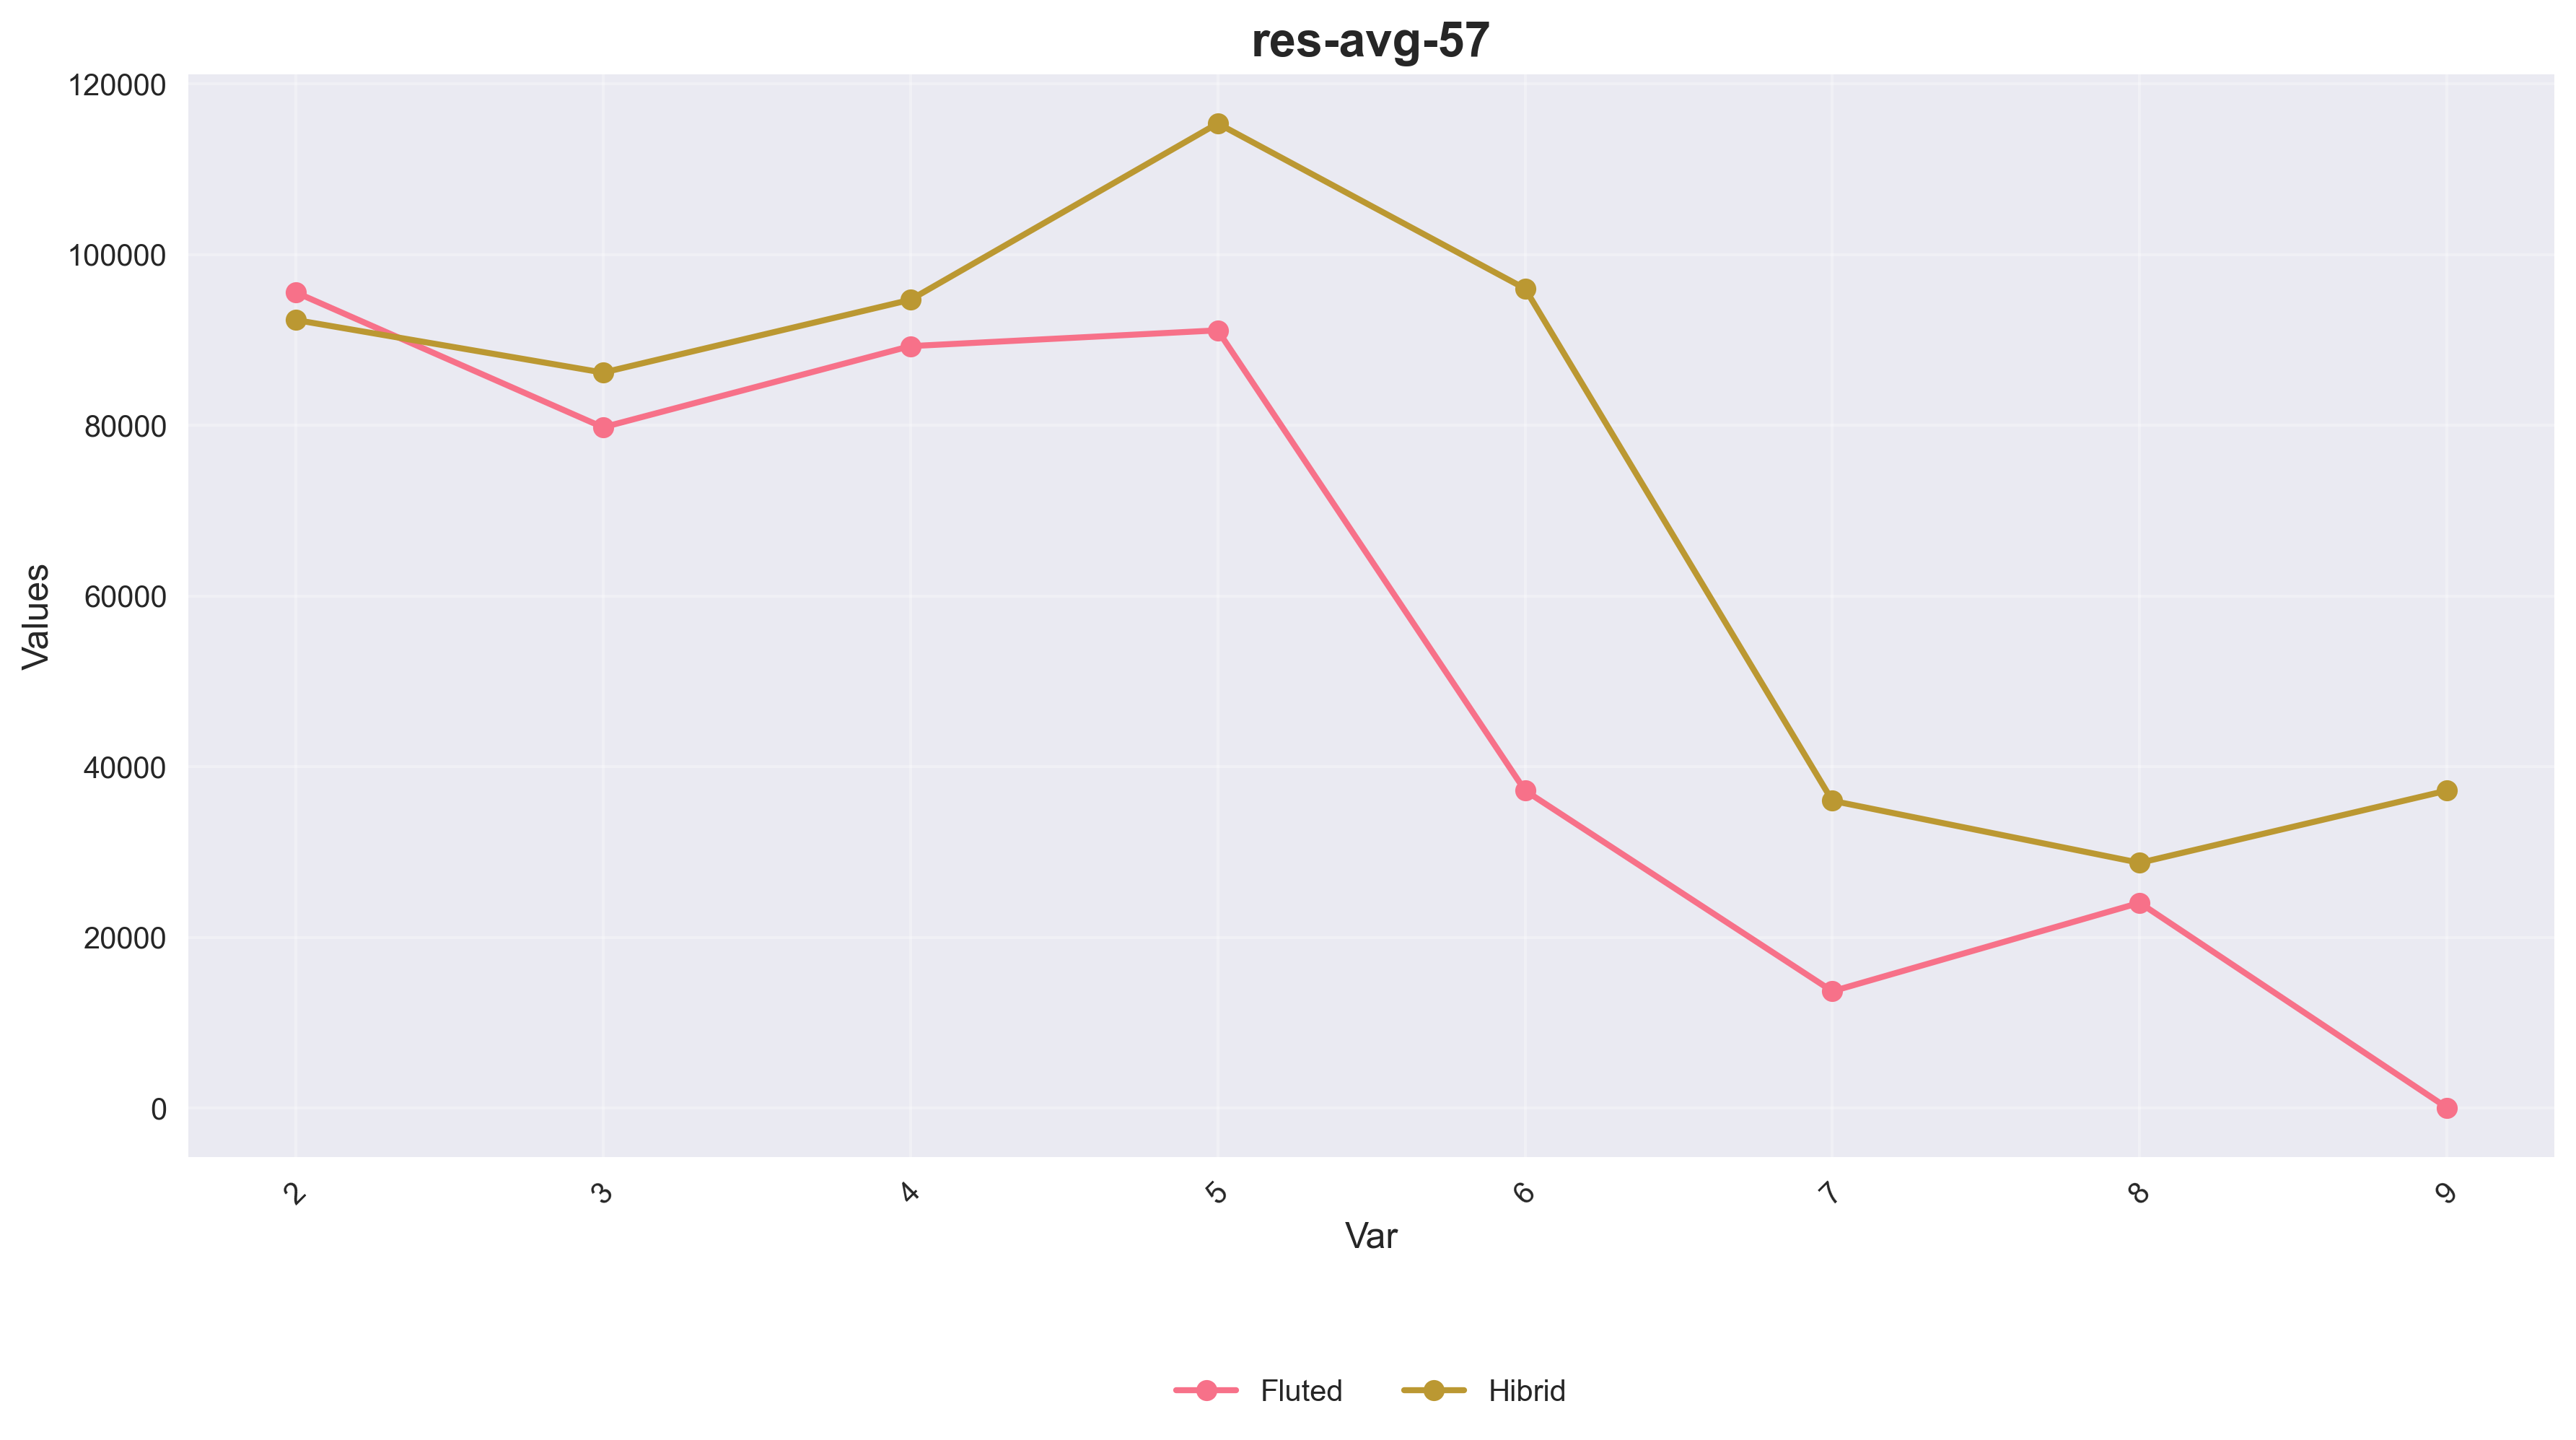
\includegraphics[width=\textwidth]{7-generated-benchmarking/aggregated/res-avg-57_linee_normal.png}
  \end{minipage}
  \caption{Aggregated results for generated problems with lexicographic encoding 57.}\label{fig:agg-le57}
\end{figure}

\begin{figure}[H]
  \centering
  \begin{minipage}{1\textwidth}
    \centering
    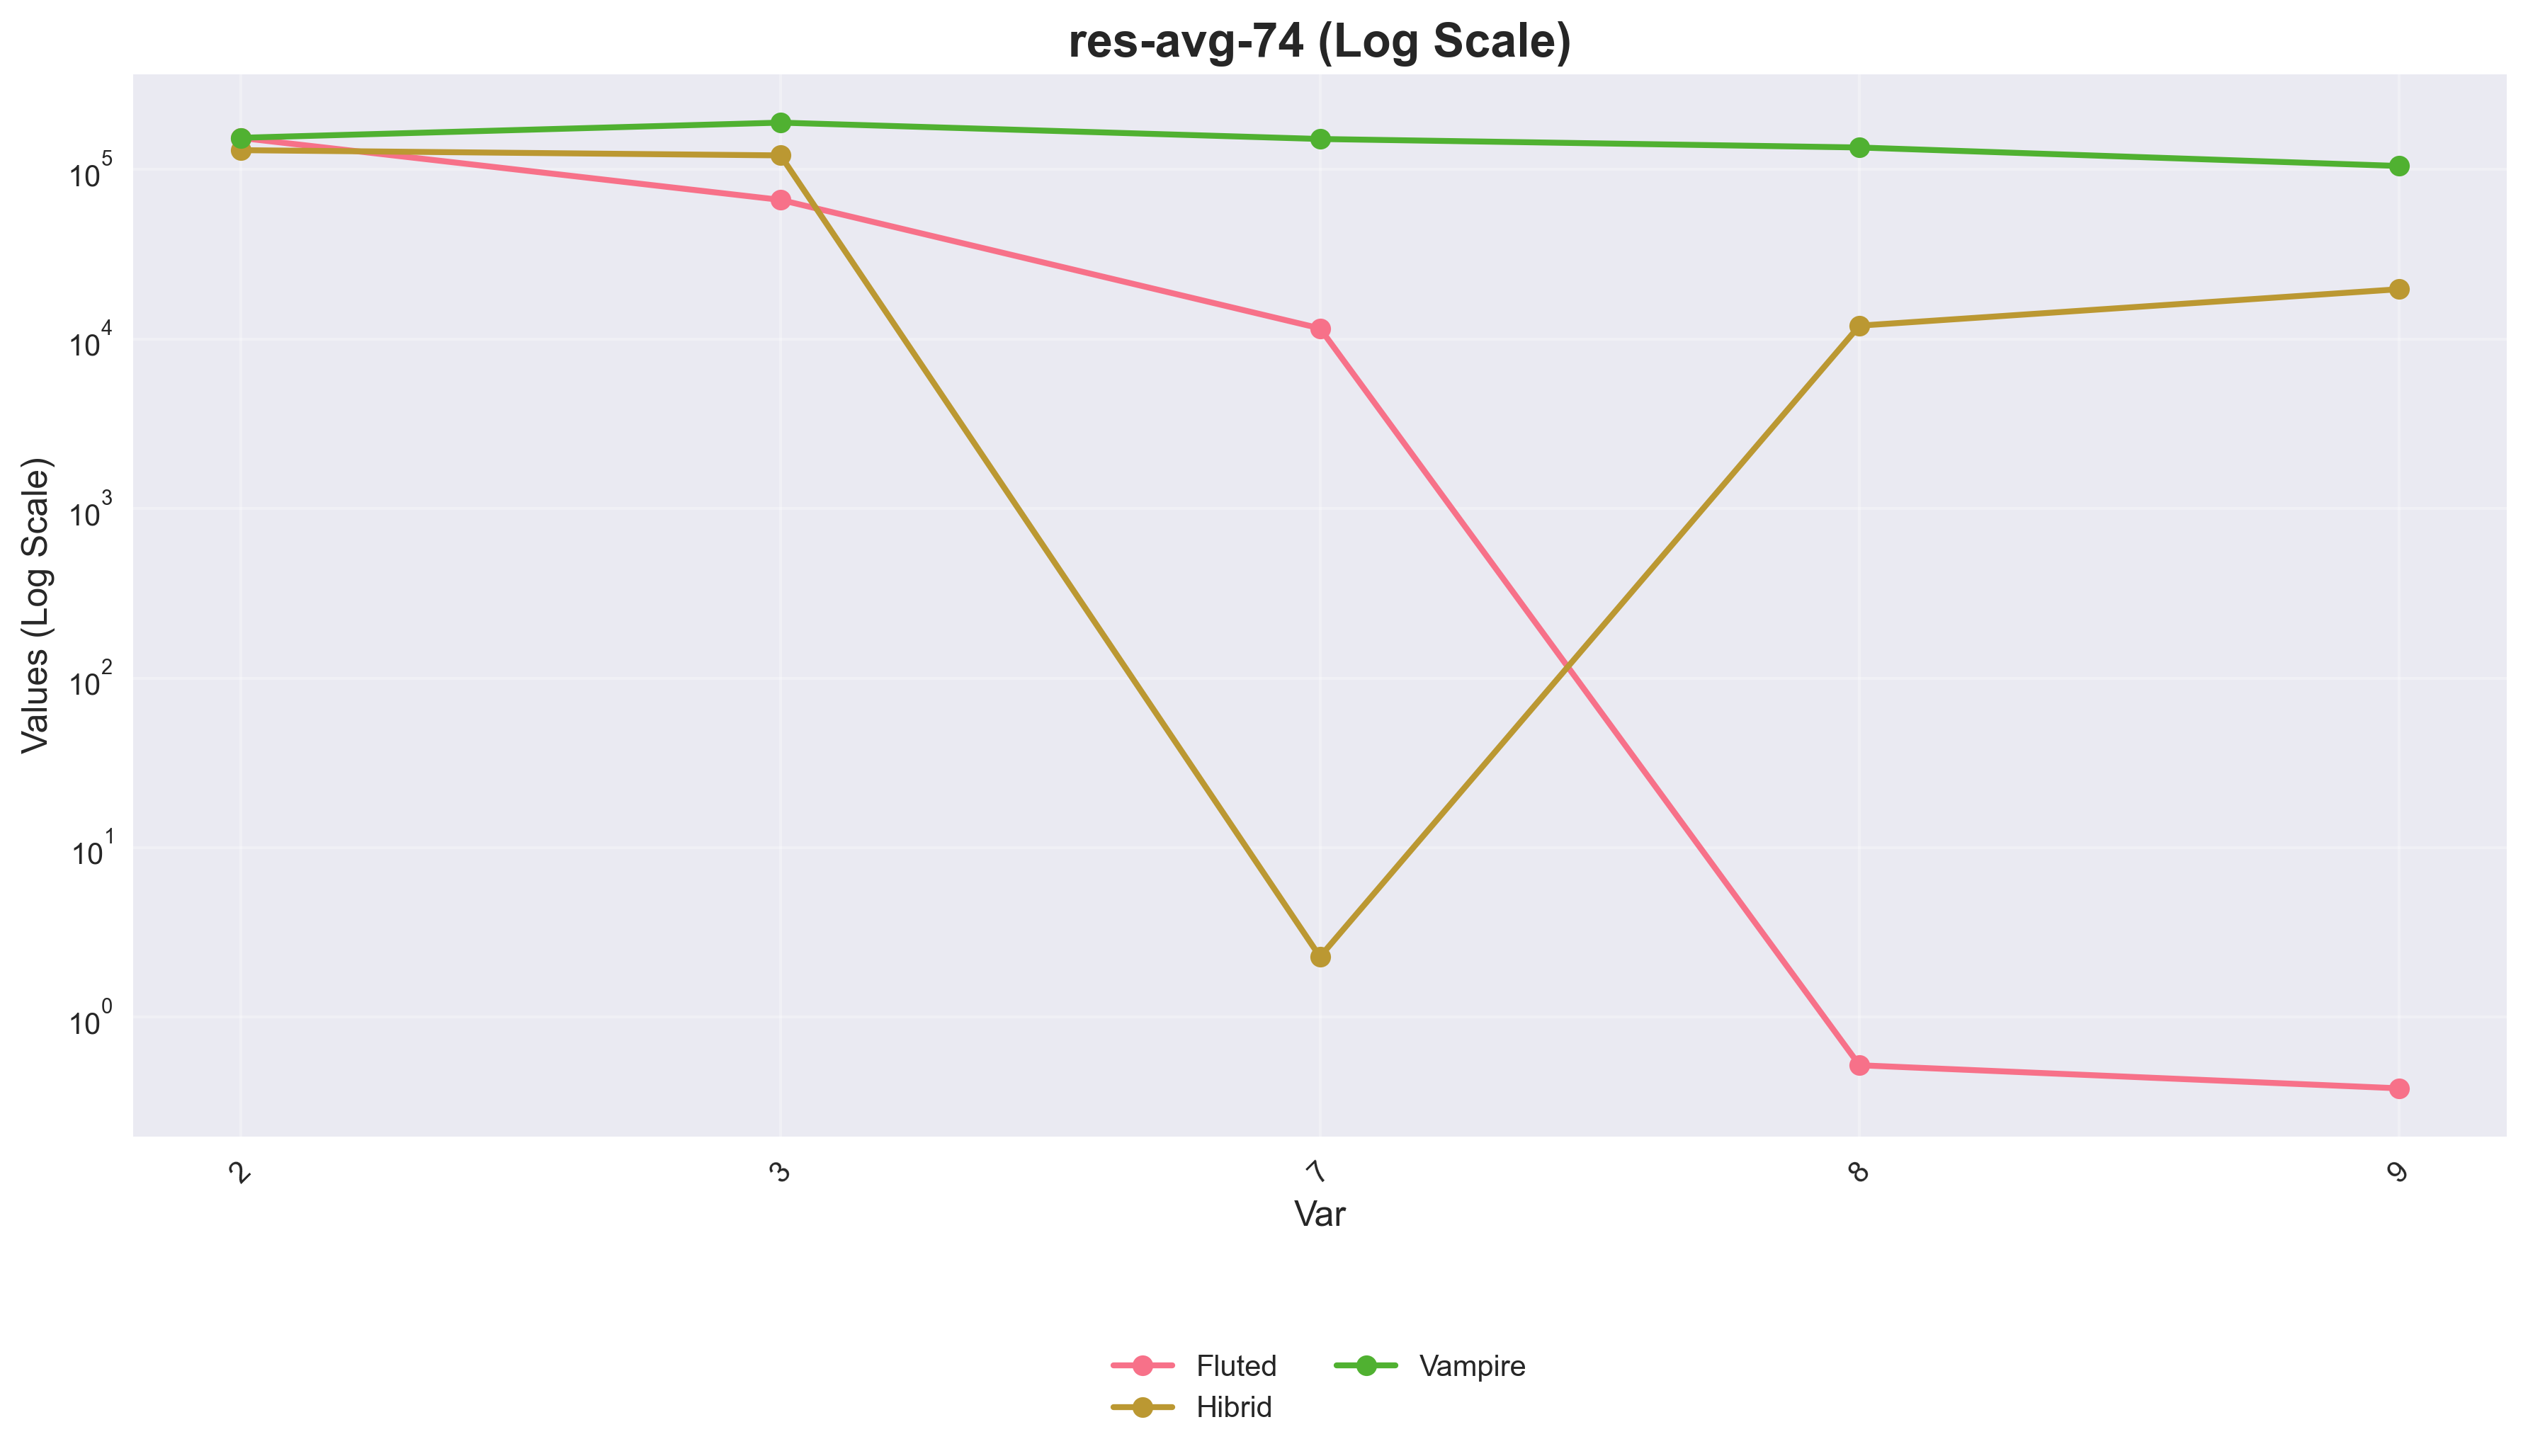
\includegraphics[width=\textwidth]{7-generated-benchmarking/aggregated/res-avg-74_linee_log.png}
  \end{minipage}
  \hfill
  \begin{minipage}{1\textwidth}
    \centering
    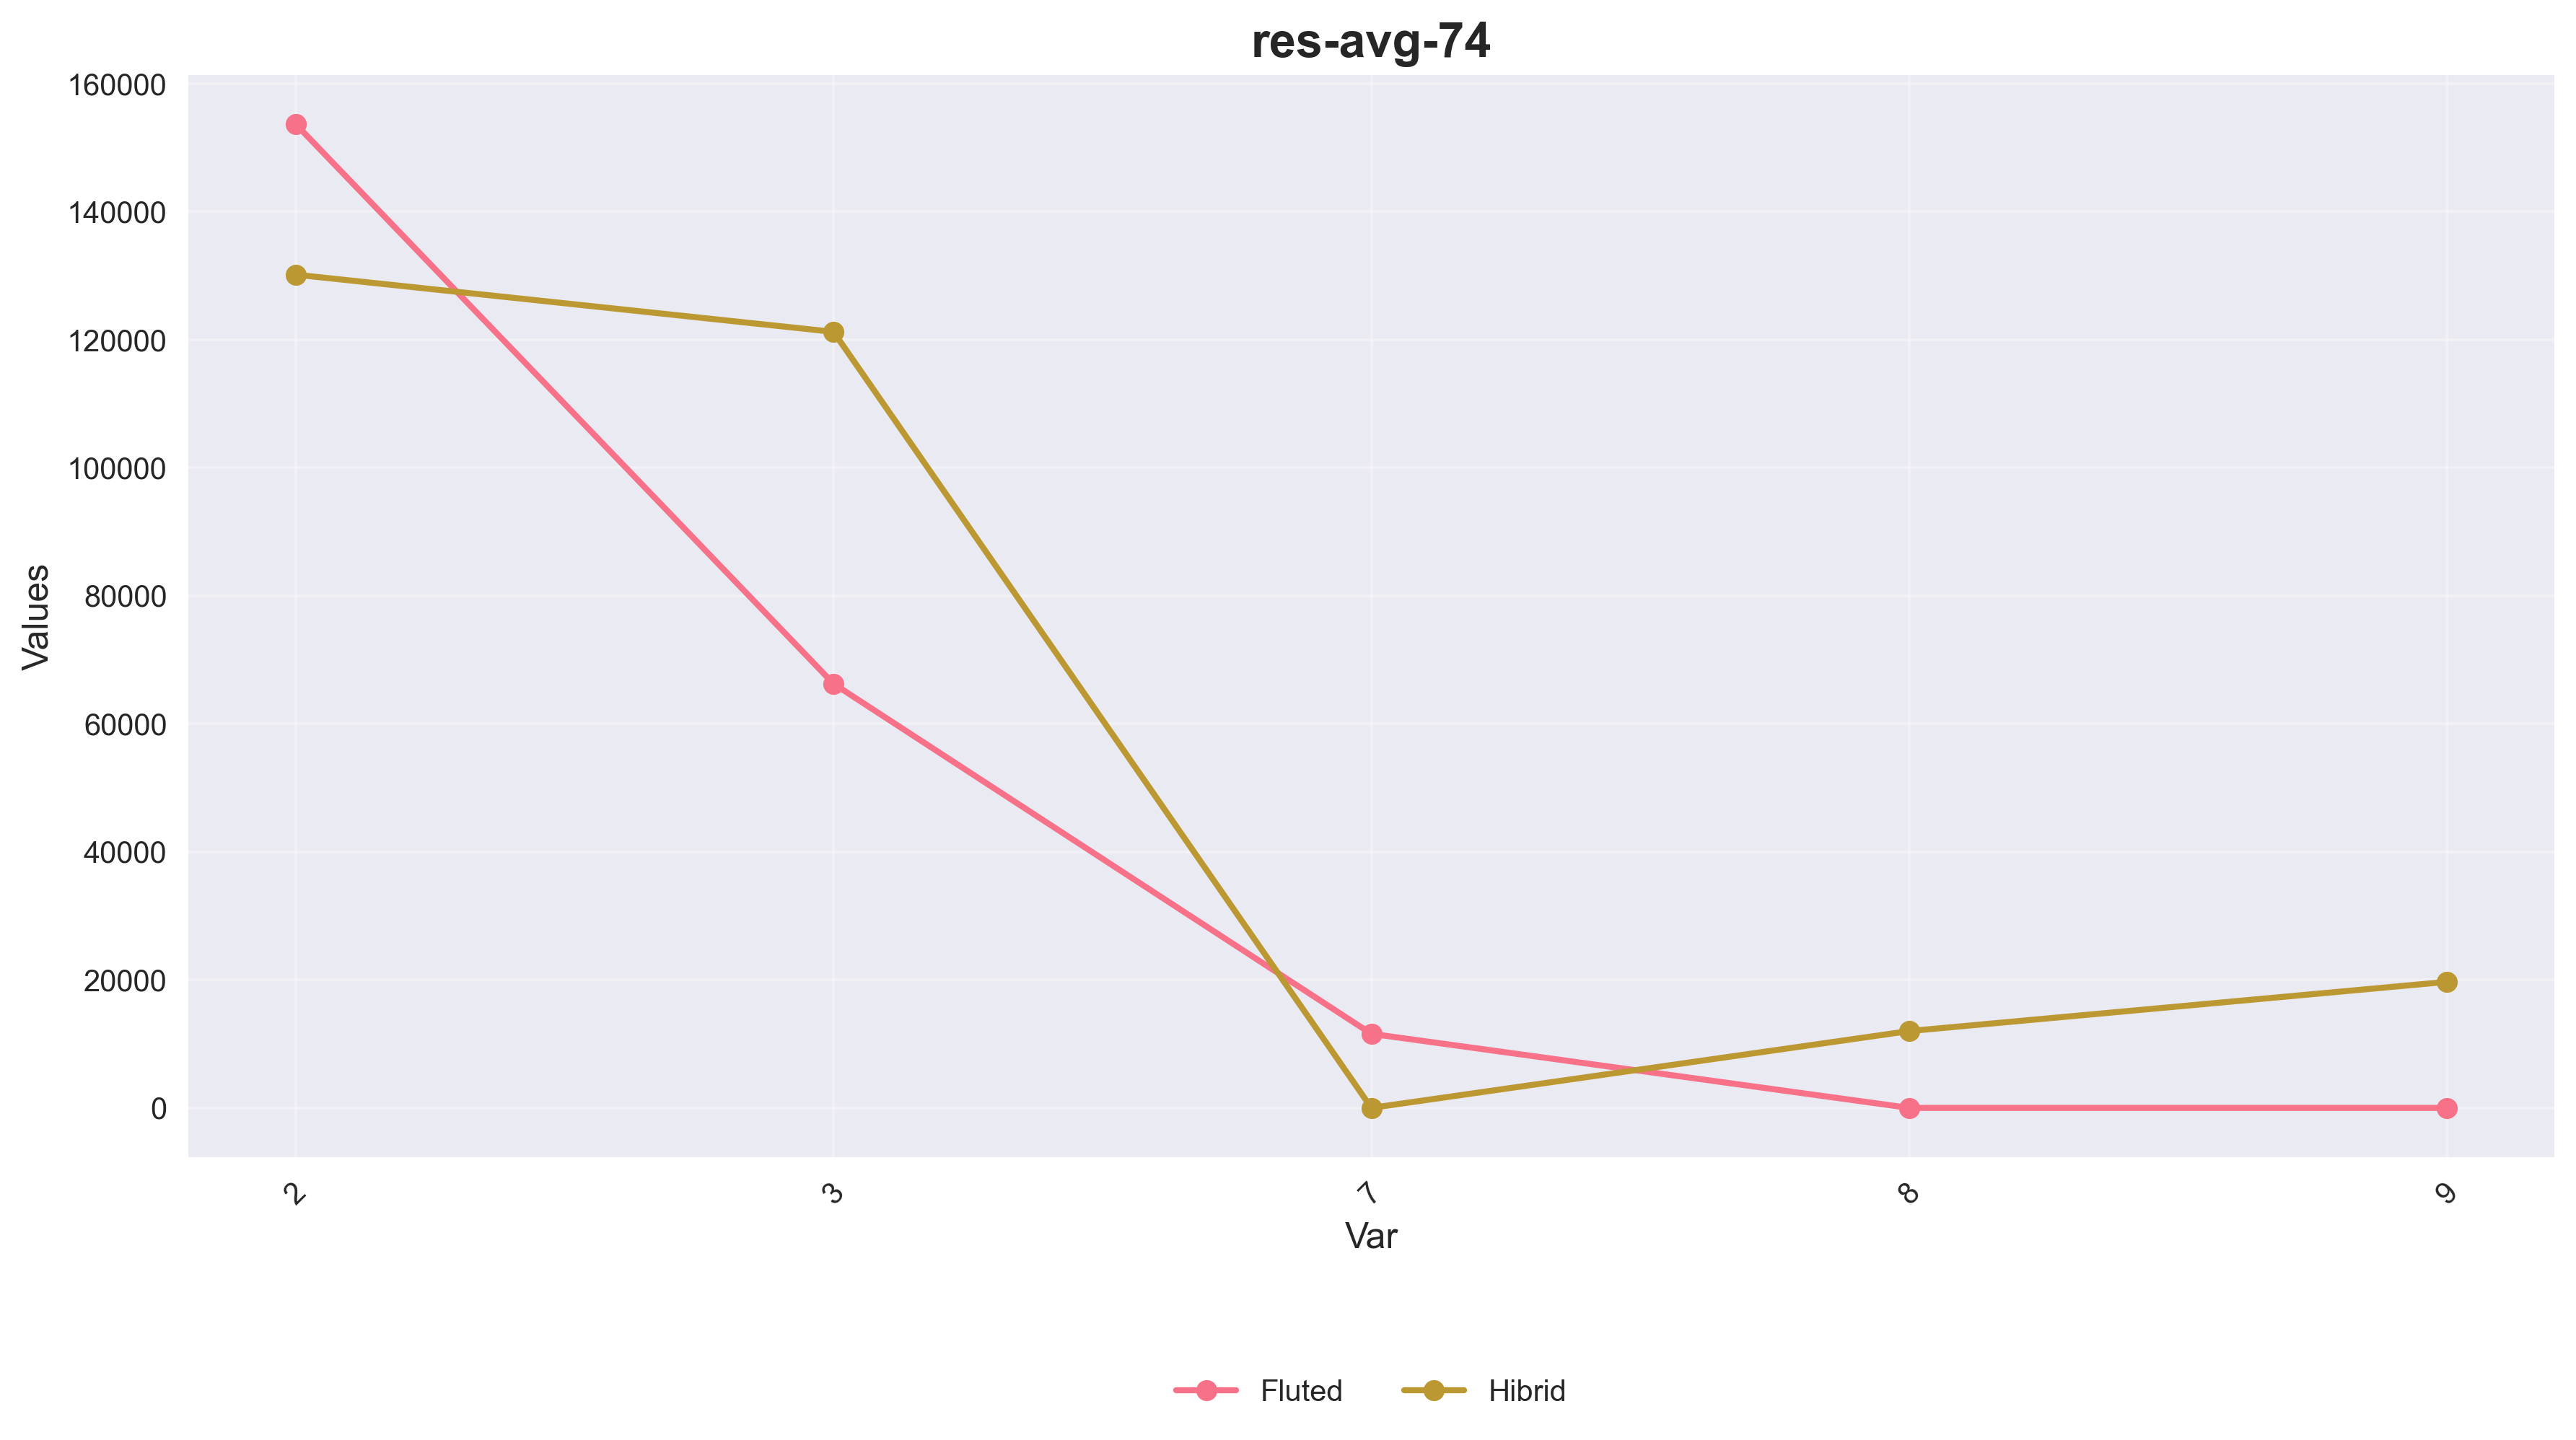
\includegraphics[width=\textwidth]{7-generated-benchmarking/aggregated/res-avg-74_linee_normal.png}
  \end{minipage}
  \caption{Aggregated results for generated problems with lexicographic encoding 74.}\label{fig:agg-le74}
\end{figure}

These charts already start to reveal some surprising trends. For confirmation, we averaged the results over all values of the other three parameters, leading to the final chart shown in Figure~\ref{fig:agg-all-vars}.
\begin{figure}[H]
  \centering
  \begin{minipage}{1\textwidth}
    \centering
    \includegraphics[width=\textwidth]{7-generated-benchmarking/aggregated/res-avg_linee_log.png}
  \end{minipage}
  \hfill
  \begin{minipage}{1\textwidth}
    \centering
    \includegraphics[width=\textwidth]{7-generated-benchmarking/aggregated/res-avg_linee_normal.png}
  \end{minipage}
  \caption{Aggregated results for generated problems over all values of \code{_predNum}, \code{_maxLen}, and \code{_unitsNum}.}\label{fig:agg-all-vars}
\end{figure}
From theoretical expectations, we would anticipate a significant increase in resolution time as the number of variables increases, given the non-elementary complexity associated with the fluted fragment.
However, the charts tell a different story. The performance seems to improve or remain relatively stable as the number of variables increases, which is counterintuitive.
This unexpected trend could be attributed to several factors, mainly related to some biases in the problem generation process.
Our hypothesis is that as the number of variables increases, less room is left for connectives and literals, leading to simpler formulae that are easier to resolve.
For example, with a maximum length of \(10\) and \(2\) variables, a formula have still \(8\) slots left, while with \(8\) variables, only \(2\) slots are left.
For solving this riddle, more in-depth analysis and testing would be required, possibly involving a more sophisticated problem generation process that can better control the complexity of the generated formulae independently of the number of variables.
An example of improvement could be to not count the quantifiers in the length of the formula (or at least the initial sequence of quantifiers), to avoid that increasing the number of variables directly decreases the number of other components in the formula.




   % other chapters here..

    \newpage\pagestyle{conclusions}
\chapter*{Conclusions and Future Work}\label{chap:conclusions}

This thesis has implemented and evaluated a decision procedure for the fluted fragment of first-order logic within the Vampire theorem prover, successfully integrating theoretical foundations with practical implementation and achieving the main objectives while revealing several interesting areas for future research.

\section*{Main Results}

The experimental evaluation demonstrates that our fluted logic decision procedure performs well in practice. Although we found only 23 CNF and 128 FOF fluted problems in the TPTP library—a limitation that makes assessing real-world applicability challenging—our implementation achieves competitive performance with standard Vampire on these naturally occurring problems.

The large-scale evaluation across 15,000 generated problems reveals more compelling results: the fluted implementation frequently outperforms standard Vampire resolution. Particularly noteworthy is the hybrid mode, which applies fluted preprocessing followed by standard resolution, as this approach demonstrates that preprocessing optimizations contribute significantly to the observed performance improvements.

These findings challenge common assumptions about specialized reasoning systems. Rather than sacrificing performance for specificity, our specialized decision procedure often provides computational advantages by exploiting structural properties inherent in fluted problems, suggesting that targeting decidable fragments can be practically worthwhile beyond their theoretical interest.

\section*{Key Insights}

The strong performance of hybrid mode reveals an important insight: techniques developed for specific fragments can benefit general-purpose reasoning as well. The preprocessing transformations we developed for fluted logic provide advantages even when falling back to standard resolution, indicating that fragment-specific optimizations may have broader applicability than initially expected.

Given the natural connection between fluted logic and modal logic systems, this implementation also provides a foundation for developing reasoning tools in modal and description logic applications, potentially avoiding the complexity explosion that occurs when translating modal problems into standard first-order logic.

\section*{Limitations and Open Questions}

Several important limitations emerged during this work that point toward areas requiring further investigation. The scarcity of naturally occurring fluted problems in standard benchmark libraries makes it difficult to assess whether the structural properties that render fluted logic theoretically attractive actually arise frequently in practical reasoning tasks.

Our problem generation methodology revealed counterintuitive patterns—sometimes increasing variable counts improved rather than degraded performance—suggesting unintended biases that contradict both theoretical expectations and practical experience with automated reasoning systems. This indicates that a more sophisticated understanding of the relationship between syntactic parameters and computational complexity would significantly improve our evaluation framework.


\section*{Future Directions}

Several promising directions emerge from this work that could substantially advance the field. The problem generation methodology requires improvement to better separate variable quantification costs from formula complexity, while developing domain-specific generators for modal logic, description logic, and natural language processing applications would provide more realistic test cases reflecting problems where fluted logic naturally arises.

From an implementation perspective, trying to use more well-integrated literal selection strategies could enhance performance. The current implementation takes a conservative approach to simplifications, so investigating the safe application of additional simplification rules, in addition to AVATAR splitting, to non-strongly fluted clauses might yield performance improvements while maintaining termination guarantees.

Theoretically, exploring relationships between fluted logic and other decidable fragments could reveal opportunities for unified approaches, while analysing complexity characteristics of different fluted clause types could inform adaptive strategy selection during resolution.

Additional technical improvements and suggestions for improvements have been mentioned throughout this thesis in the relevant sections.

\section*{Final Thoughts}

This work demonstrates that the fluted fragment represents a meaningful balance between expressiveness and computational tractability, with the successful implementation within Vampire showing that theoretical insights about decidable fragments can translate effectively into practical computational tools.

While representing just one specialized reasoning technique, this work illustrates the broader potential for enhancing modern theorem provers through optimizations that respect structural characteristics of specific problem classes. As automated reasoning assumes increasingly important roles in computer science applications, techniques that exploit structural properties of input problems become correspondingly more valuable.

The methodology combining theoretical study, practical implementation, and systematic experimental evaluation provides a reusable approach for investigating other fragments and developing targeted optimizations. This contribution advances that goal by demonstrating that specialized reasoning can achieve both theoretical soundness and practical benefits.

    %appendix title style
\titleformat{\chapter}[block]{\Huge\bfseries}{
    \sffamily\huge\centering{Appendix \thechapter{}
}\\}{1ex}{\sffamily\centering\huge\bfseries}

\newpage\pagestyle{appendices}
\begin{appendices}

\chapter{This is an appendix}\label{appendix}
\section{Appendix section}

\section{Appendix section}


%now another appendix

\end{appendices}
    
    \newpage
    \pagestyle{backmatter}
    \printbibliography[heading=bibintoc]
    

    %\listoffigures
 
    %\listoftables

\end{document}